% ------------------------------------------------------------------
%
%   TITLE: LIQUID documentation
% AUTHORS: Joseph D. Gaeddert et al.
% CREATED: February 7, 2009
% REVISED: 
%     URL: http://liquidsdr.org/
%
% ------------------------------------------------------------------
 
\documentclass[11pt,twoside]{article}

% ------------------- DOCUMENT VARIABLES -------------------
\setlength{\textwidth}{6.5in}
\setlength{\textheight}{8.5in}
\setlength{\evensidemargin}{0in}
\setlength{\oddsidemargin}{0in}
\setlength{\topmargin}{0in}
%\setlength{\parindent}{0pt}
%\setlength{\parskip}{0.1in}


% ------------------- BIBLIOGRAPHY STYLE -------------------
\usepackage{natbib}
\bibliographystyle{plain} % note the change here
\bibpunct{[}{]}{,}{n}{}{;}  % define bibliography punctuation
% The six mandatory arguments for \bibpunct are:
%   1. opening bracket: '(', '[', '{', or '<'
%   2. closing bracket: ')', ']', '}', or '>'
%   3. separator between multiple citations: ';' or ','
%   4. citation style: 'n' for numerical style, 's' for numerical superscript
%      style, or 'a' for author year style
%   5. punctuation between the author names and the year
%   6. punctuation between years or numbers when common author lists are suppressed: ',' or ';' 

% ------------------- GRAPHICS PACKAGES -------------------
%\usepackage{epsf}
%\usepackage{graphicx}
\ifx\pdfoutput\undefined
\usepackage{graphicx}
\else
\usepackage[pdftex]{graphicx}
\fi
\usepackage{epsfig}
\usepackage{epstopdf}
\usepackage{colortbl}
\usepackage{color}

%\usepackage{tabularx}
\usepackage{ctable} % \toprule, \midrule, \bottomrule
\setlength{\heavyrulewidth}{0.1em} % modify thickness of \toprule, \bottomrule
\newcommand{\otoprule}{\midrule[\heavyrulewidth]}
\usepackage{subfigure}
\usepackage{multirow} % for tables
%\usepackage{fancyhdr}
\usepackage{amsmath}
\usepackage{amssymb}
\usepackage{listings}
\usepackage{fancyvrb}
\usepackage{acronym}

% define colors here
\definecolor{liquid-color-blue}{rgb}{  0.00, 0.25, 0.50}
\definecolor{liquid-color-green}{rgb}{ 0.00, 0.50, 0.25}
\definecolor{liquid-color-red}{rgb}{   0.50, 0.00, 0.00}
\definecolor{liquid-color-purple}{rgb}{0.25, 0.00, 0.25}
\definecolor{liquid-color-grid}{rgb}{  0.90, 0.90, 0.90}
\definecolor{liquid-color-gray}{rgb}{  0.50, 0.50, 0.50}

% http://en.wikibooks.org/wiki/LaTeX/Hyperlinks
\usepackage{hyperref}
\hypersetup{
    bookmarks=true,                     % show bookmarks bar?
    pdfborder={0 0 0},                  % set border around each link
    pdftitle={liquid-dsp},              % title
    pdfauthor={Joseph D. Gaeddert},     % author
    colorlinks=true,                    % false: boxed links; true: colored links
    linkcolor=liquid-color-blue,        % color of internal links
    citecolor=liquid-color-green,       % color of links to bibliography
    filecolor=liquid-color-red,         % color of file links
    urlcolor=liquid-color-purple        % color of external links
}

% defines compact itemize*, enumerate*, and description* environments
% http://www.ctan.org/tex-archive/help/Catalogue/entries/mdwtools.html
%\usepackage{mdwlist}

% cleveref package, http://www.ctan.org/tex-archive/macros/latex/contrib/cleveref/
%\usepackage[capitalize]{cleveref}

% tabular: \hline (thin) \hline\hline (thick)
% from: http://www.faqs.org/faqs/tex-faq/ (see #44)
\setlength{\doublerulesep}{\arrayrulewidth}

%--------- CAPTION OPTIONS -------------------
\usepackage[small,bf]{caption}
\setcaptionwidth{15cm}
\setlength{\belowcaptionskip}{0.5cm}


% algorithms
%   http://tug.ctan.org/tex-archive/macros/latex/contrib/algorithms/
\usepackage{algorithm}
\usepackage{algorithmic}
% customized algorithm comments
%\renewcommand{\algorithmiccomment}[1]{// #1}
\definecolor{algorithm-comment-color}{rgb}{0.7,0.7,0.7}
\renewcommand{\algorithmiccomment}[1]{\textcolor{algorithm-comment-color}{\sf \,\, (#1)}}

% 
% TikZ options
%
\usepackage{tikz}
\usetikzlibrary{decorations.pathreplacing} % brace
\usetikzlibrary{decorations.pathmorphing}
\usetikzlibrary{shapes}
\usetikzlibrary{patterns}
\usetikzlibrary{positioning}


%--------- NEW COMMANDS -------------------
\newcommand{\NA}{\scriptsize{NA}}
\newcommand{\E}{\scriptsize{E}}
\newcommand{\tRMS}{\ensuremath{\tau_{rms}}}
\newcommand{\tmED}{\ensuremath{\bar{\tau}}}
\newcommand{\Np}{\ensuremath{N_p}}
\newcommand{\ua}{\ensuremath{\uparrow}}
\newcommand{\da}{\ensuremath{\downarrow}}
\newcommand{\sinc}{\textup{sinc}}
\newcommand{\erf}{\textup{erf}}
\newcommand{\etal}{{\it et al.}}
\newcommand{\wavt}{W@VT}
\renewcommand{\vec}[1]{\boldsymbol{#1}}
\newcommand{\ciren}{C{\sc iren}}
\newcommand{\ord}{\mathcal{O}}
\newcommand{\F}{\mathcal{F}}        % Fourier transform
\newcommand{\Ss}{\ensuremath{\mathcal{S}_0}}     % ofdmframe: short sequence
\newcommand{\Sl}{\ensuremath{\mathcal{S}_1}}     % ofdmframe: long sequence
\newcommand{\liquid}{{\it liquid}}
\newcommand{\liquidfpm}{{\it liquid-fpm}}
% include auto-generated version (LIQUID_VERSION from include/liquid.h),
% defines: \newcommand{\liquidversion}{X.Y.Z}
\input{latex.gen/liquid_version.tex}

%--------- COUNTERS -------------------
\setcounter{MaxMatrixCols}{20}  % maximum matrix columns


%%%%%%%%%%%%%%%%%%%%%%%%%%%%%%%%%%%%%%%%%%%%%%%%%%%%%%%%%%%%%%%%%%%%%
%
%             MAIN DOCUMENT
%
%%%%%%%%%%%%%%%%%%%%%%%%%%%%%%%%%%%%%%%%%%%%%%%%%%%%%%%%%%%%%%%%%%%%%

\begin{document}

% ------------------- DEFINE LISTINGS -------------------
\input{highlight.sty}


%%%%%%%%%%%%%%%%%%%%%%%%%%%%%%%%%%%%%%%%%%%%%%%%%%%%%%%%%%%%%%%%%%%%%
%
%             TITLE PAGE
%
%%%%%%%%%%%%%%%%%%%%%%%%%%%%%%%%%%%%%%%%%%%%%%%%%%%%%%%%%%%%%%%%%%%%%
\thispagestyle{empty}
\pagenumbering{roman}
\begin{center}

\includegraphics[width=\textwidth]{graphics/liquid_splatter_00.png}
\end{center}

\vfill

\noindent
{\huge\it liquid}

\noindent
software-defined radio digital signal processing library

\vfill

\noindent
User's Manual for Version \liquidversion

\vfill

\noindent
Joseph D. Gaeddert \\
\today \\
Blacksburg, Virginia \\
{\tt liquid@vt.edu}
%\begin{Verbatim}[fontsize=\small,formatcom=\color{algorithm-comment-color}]
%$ git clone git://github.com/jgaeddert/liquid-dsp.git liquid-dsp
%$ cd liquid-dsp
%$ ./bootstrap.sh
%$ ./configure
%$ make
%# make install
%\end{Verbatim}

%{\it Keywords:}
%polyphase filterbanks,
%OFDM/OQAM,
%power consumption,
%cognitive radio,
%software-defined radio,
%dynamic spectrum access

\vfill

\noindent
{\footnotesize This entire project was proudly coded using {\em Vim} and {\tt gcc}}

\pagebreak
%%%%%%%%%%%%%%%%%%%%%%%%%%%%%%%%%%%%%%%%%%%%%%%%%%%%%%%%%%%%%%%%%%%%%
%
%             TABLE OF CONTENTS
%
%%%%%%%%%%%%%%%%%%%%%%%%%%%%%%%%%%%%%%%%%%%%%%%%%%%%%%%%%%%%%%%%%%%%%
\tableofcontents
\pagebreak

%\listoffigures
%\pagebreak

%\listoftables
%\pagebreak

%\section*{List of Abbreviations}
%\begin{acronym}
%  \acro{AWGN}{additive white Gauss noise}
%\end{acronym}

\pagenumbering{arabic}
\pagestyle{headings}

%%%%%%%%%%%%%%%%%%%%%%%%%%%%%%%%%%%%%%%%%%%%%%%%%%%%%%%%%%%%%%%%%%%%%
%
%             Introduction
%
%%%%%%%%%%%%%%%%%%%%%%%%%%%%%%%%%%%%%%%%%%%%%%%%%%%%%%%%%%%%%%%%%%%%%

\newpage
\part{Introduction to \liquid }
\label{part:intro}

\bigskip
\noindent
The next few sections are designed to give you an understanding of
\liquid's intended purpose and where it might fit within your project.
Included is a quick start guide, example source code, and a brief
historical outline.

\vfill


\includegraphics[width=\textwidth]{graphics/liquid_splatter_01.png}

\vfill


%
% introduction
%

\section{Key points}
\begin{itemize}
\item open-source software-defined radio DSP algorithms
\item minimal dependence on external libraries
\item portable to embedded platforms
\item flexible configuration
\item targets cognitive radios and enabling technologies through
      flexible algorithmic development
\end{itemize}

\subsection{Features}
\begin{itemize}
\item automatic test scripts for validation and accuracy
\item benchmark tool for estimating computational speed on your machine
\end{itemize}


\section{Quick Start Guide}
To build:
\begin{verbatim}
cd /path/to/liquid/
./reconf
./configure
make
sudo make install
\end{verbatim}
You may also want to build and run the optional validation program via
\begin{verbatim}
make check
\end{verbatim}
and the benchmarking tool,
\begin{verbatim}
make bench
\end{verbatim}

\section{Tutorial}
Most of {\it liquid}'s signal processing elements are C structures which
retain the object's parameters, state, and other useful information.
The naming convention is
{\tt basename\_xxxt\_method} where
{\tt basename} is the base object name (e.g. {\tt interp}),
{\tt xxxt} is the type definition, and
{\tt method} is the object method.
The type definition describes respective output, internal, and input type.
Types are usually {\tt f} to denote standard 32-bit {\it floating point}
precision values and can either be represented as {\tt r} (real) or {\tt c}
(complex).
For example, a {\tt dotprod} (vector dot product) object with complex input
and output types but real internal coefficients operating on 32-bit
floating-point precision values is {\tt dotprod\_crcf}.

Most objects have at least four standard methods:
{\tt create()},
{\tt destroy()},
{\tt print()},
and
{\tt execute()}.
Certain object also implement a {\tt recreate()} method which operates similar
to that of {\tt realloc()} in C.
A few points to note:
\begin{enumerate}
\item While the objects do retain internal memory, they operate on external
arrays defined by the user. That is... It is strictly up to the user to manage
his/her own memory.
\item ...
\end{enumerate}

\section{Learning by example}
The {\tt examples/} subdirectory includes numerous examples for nearly all the
signal processing components.

\section{Sandbox}

\subsection{Why C?}
A commonly asked question is ``why C and not C++?''
The answer is simple: {\em portability}.
Our aim is to provide a lightweight DSP library for software-defined radio
that does not rely on a myriad of dependencies.
While C++ is a fine language for many purposes (and theoretically runs just as
fast as C), it is not as portable to embedded platforms as C.
Furthermore, the majority of functions simply perform complex operations on a
data sequence and do not require a high-level object-oriented programming
interface.
This we will leave to framework developers and interface builders.

While a number of signal processing elements in \liquid\ use structures, these
are simply to save the internal state of the object.
For instance, a {\tt firfilt\_crcf} (finite impulse response filter) object
is just a structure which contains--among other things--the filter taps
(coefficients) and an input buffer.
For the most part, C++ polymorphic data types and abstract base classes are
unnecessary for basic signal processing, and primarily serve to reduce the
code base of a project.
Furthermore, while templates can certainly be useful for library development,
their benefits are of limited use to signal processing and can be circumvented
through the use of pre-processor macros at the gain of targeting more embedded
processors.

The C programming language has a rich history in system programming--
specifically targeting embedded applications--and is the basis behind many
well-known projects including the linux kernel and the python programming
language.

\subsection{Data Types}
The majority of signal processing for SDR is performed at complex baseband.
Complex numbers are handled in \liquid\ by defining data type
{\tt liquid\_float\_complex} which is binary compatible with the standard
C math type {\tt float complex} and C++ type {\tt std::complex<float>}.

Fixed-point data types are defined in the \liquidfpm\ library (see XXX).

\subsection{Building/Linking with C++}
Although \liquid\ is written in C, it can be seamlessly compiled and linked
with C++ source files.
Here is an example:
\input{listings/nco.c++.tex}

\section{History}
\liquid\ was created by J. Gaeddert out of necessity to perform complex
digital signal processing algorithms on embedded devices
without relying on dealing
with proprietary and otherwise cumbersome frameworks.
This was a critical step in his PhD thesis to adapt DSP algorithms in
cognitive dynamic-spectrum radios to optimally manage finite radio resources.
Was he successful?
Put it this way: at the time this document was written he still has not
graduated.\footnote{Come back in a year and ask again... {\em sigh}}




%%%%%%%%%%%%%%%%%%%%%%%%%%%%%%%%%%%%%%%%%%%%%%%%%%%%%%%%%%%%%%%%%%%%%
%
%             Tutorials
%
%%%%%%%%%%%%%%%%%%%%%%%%%%%%%%%%%%%%%%%%%%%%%%%%%%%%%%%%%%%%%%%%%%%%%
\newpage
\part{Tutorials}
\label{part:tutorials}

\bigskip
\noindent
To get you started with using \liquid\ signal processing library
this manual begins with tutorials rather than diving into the details of
each signal processing module.
%
The tutorials begin with simple building blocks for signal processing by
introducing a simple analog {\bf phase-locked loop} which tracks to the
phase of an input complex sinusoid.
%
% TODO: insert modem tutorial
%
The {\bf forward error-correction tutorial}
introduces you to simple error correction and detection
capabilities.
%
The {\bf framing tutorial}
puts together data encapsulation with digital modulation;
with just a few lines of code you can convert a block of raw, unencoded
data bytes to frame samples ready to transmit over the air.
%
Last but not least is the {\bf OFDM framing tutorial}
which builds on the previous tutorial to use an orthogonal parallel
multiplexing communications scheme.
%Furthermore, certain aspects of the transmission can be changed on a
%per-frame basis without requiring you to re-configure the synchronizer;
%this happens automatically.
%
Detailed examples of nearly every module can be found in the
{\tt examples} directory.

\vfill

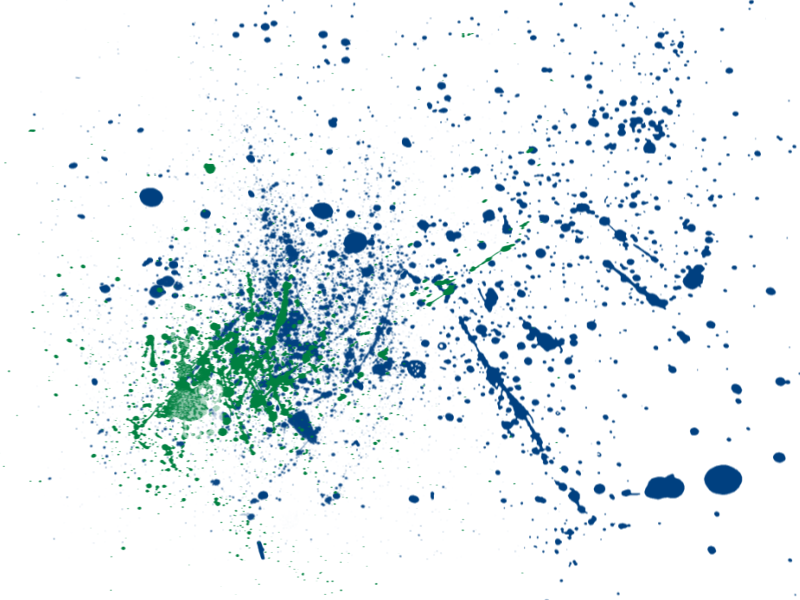
\includegraphics[width=\textwidth]{graphics/liquid_splatter_02.png}

\vfill


% 
% TUTORIAL : pll
%

\newpage
\section{Tutorial: Phase-Locked Loop}
\label{tutorial:pll}
This tutorial demonstrates the functionality of a carrier phase-locked
loop and introduces the {\tt iirfilt} object.
%
You will need on your local machine:
\begin{itemize}
\item the \liquid\ DSP libraries built and installed
\item a text editor such as {\tt vim} \cite{vim:web}
\item a C compiler such as {\tt gcc} \cite{gcc:web}
\item a terminal
\end{itemize}

\subsection{Problem Statement}
\label{tutorial:pll:problem}
Wireless communications systems up-convert the data signal with
a high-frequency carrier before transmitting over the air.
This transmitted signal is orthogonal to other signals so long as
their bandwidths don't overlap and can be recovered at the receiver by
mixing it back down to baseband.
%This is accomplished by mixing the complex baseband signal...
%with a complex sinusoid, viz
%\[
%    s(t) = \Re\Bigl\{ m(t)\exp\{j\omega_ct\} \Bigr\}
%\]
Many digital communications systems modulate information in the phase of
the carrier requiring the receiver to demodulate the signal coherently
in order to recover the original data message.
In this regard the receiver must synchronize its carrier oscillator to
that of the transmitter.
To put it simply, the receiver must lock on to the phase of
transmitter's carrier.
One of the key advantages to performing signal processing in software is
that the radio can operate at complex baseband.
% TODO : expand on this
% (see Section~\ref{section:complex_baseband}).

In this simulation, the received signal is simply a complex sinusoid
with an unknown initial carrier phase and frequency.
The carrer holds no information-bearing symbols and is simply a tone
whose frequency and phase represent the residual mismatch between the
transmitter and receiver.
The received signal $x$ at time step $i$ can be described as
%
\begin{equation}
\label{eqn:tutoral:pll:x}
    x_i = \exp\bigl\{ j(\theta + i\omega) \bigr\}
\end{equation}
%
where $j \triangleq \sqrt{-1}$ and
$\theta$ and $\omega$ represent the unknown initial carrier phase and
frequency offsets, respectively.
The receiver generates a complex sinusoid with a phase $\phi_i$ as the
phase difference between $x_i$ and $y_i$ and can be computed as
%
\begin{equation}
\label{eqn:tutoral:pll:y}
    y_i = \exp\bigl\{j\phi_i\bigr\}
\end{equation}
%
%which tries to minimize the difference between the phase of the ...
The phase error at time step $i$ is expressed as
%
\begin{equation}
\label{eqn:tutoral:pll:dphi}
    \Delta\phi_i = \arg\bigl\{ x_i y_i^* \bigr\}
\end{equation}
%
where $(^*)$ denotes complex conjugation.%
\footnote{
    Those who are savvy with communications techniques will
    appreciate that we are dealing in complex baseband and can easily
    compute the phase error estimate simply as the argument of the
    product of $x_i$ and $y_i$.
    Conventional PLLs which have operated strictly in the real domain
    multiply only the real components of $x_i$ and $y_i$ for a phase
    error estimate, assume that the loop filter rejects the
    high-frequency component, and make the approximation
    $\Delta\phi \approx \sin(\Delta\phi) = \sin(\phi-\hat{\phi})$
    for small phase errors.}
The goal of the receiver is to control $\phi_i$
(the phase of the output signal $y$ at time $i$)
to lock onto the input phase of $x$,
hence the name ``phase-locked loop.''
If the phase of the output sample $y_i$ is behind that of the input
($\Delta\phi > 0$) then $\phi$ needs to be advanced appropriately for
the next time step.
Conversely, if the phase of $y_i$ is ahead of the phase of $x_i$
($\Delta\phi < 0$) then the receiver need to retard $\phi$.

Without going into a great amount of detail, this control is
accomplished using a special filter within the loop.
This filter, known as a ``loop filter,'' is designed to reject
high-frequency noise and is described with the transfer function $H(z)$.
Specifically $H(z)$ is a 2$^{nd}$-order integrating low-pass recursive
filter with
a natural frequency $\omega_n$,
a damping factor $\zeta$, and
a loop gain $K$.
The natural frequency is the resonant frequency of $H(z)$ and for all
practical purposes is the filter's bandwidth.
Increasing $\omega_n$ permits the loop to track to the input signal
faster (reduces lock time), but also increases the amount of noise
passed through the loop.
Decreasing $\omega_n$ reduces this noise but also increases the loop's
acquisition time.
The damping factor $\zeta$ controls the stability of the filter and is
typically set to a value near $1/\sqrt{2} \approx 0.707$.
The loop gain $K$ is typically very large
(on the order of $1000$ or so).
For more detailed information on loop filter design the interested
reader is referred to Section~\ref{module:nco:pll}.
% TODO : reference iirdes_pll_...() as well?

The estimated phase error $\Delta\phi$ is filtered using $H(z)$
resulting in an output phase estimate $\phi_{i+1}$
which is used for the subsequent output sample $y_{i+1}$ as
%
\begin{equation}
\label{eqn:tutoral:pll:y1}
    y_{i+1} = \exp\bigl\{ j\phi_{i+1} \bigr\}
\end{equation}
%
%A summary of the algorithm is:
%
%parameters:
%    $ x = \bigl\{x_0, x_1, x_2, \ldots \bigr\}$ (input array)
%
%initialization:
%    $ \hat{\phi}_0 = 0 $ (initial output phase)
%
%computation: for $i=0, 1, 2, \ldots$
%       $y_i = \exp\bigl\{ j*\hat{\phi}_i \bigr\}$
%       $\Delta\phi_i = \arg\bigl\{ x_i y_i^* \bigr\}$ % phase detector
%       $\hat{\phi}_{i+1} = \text{filter}(\Delta\phi_i)$
%
In the next section we will create a simple C program to simulate a
phase-locked loop with \liquid.


\subsection{Setting up the Environment}
\label{tutorial:pll:environment}

For this tutorial and others, I assume that you are using the GNU
compiler collection ({\tt gcc}) for compiling source and linking objects
\cite{gcc:web},
and that you have a familiarity with the C (or C++) programming
language.
Create a new file {\tt pll.c} and open it with your favorite editor.
Include the headers {\tt stdio.h}, {\tt complex.h}, {\tt math.h}, and
{\tt liquid/liquid.h} and add the {\tt int main()} definition
so that your program looks like this:
%
\input{tutorials/pll_init_tutorial.c.tex}
%
Compile and link the program using {\tt gcc}:
%
\begin{Verbatim}[fontsize=\small]
    $ gcc -Wall -o pll -lm -lc -lliquid pll.c
\end{Verbatim}
%
The flag ``{\tt -Wall}'' tells the compiler to print all warnings
(unused and uninitialized variables, etc.),
``{\tt -o pll}'' specifies the name of the output program is
``{\tt pll}'', and
``{\tt -lm -lc -lliquid}'' tells the linker to link the binary against
the math, standard C, and \liquid\ DSP libraries, respectively.
Notice that the above command invokes both the compiler and the linker
collectively.
%While it is usually preferred to build an intermediate object...
%
If the compiler did not give any errors, the output executable {\tt pll}
is created which can be run as
\begin{Verbatim}[fontsize=\small]
    $ ./pll
\end{Verbatim}
%
and should simply print ``{\tt done.}'' to the screen.
You are now ready to add functionality to your program.

We will now edit the file to set up the basic simulation but without
controlling the phase of the output sinusoid.
As such the output won't track to the input resulting in a significant
amount of phase error.
This simulation will operate one sample at a time and is organized into
three sections.
First, set up the simulation parameters: the initial phase and frequency
offsets ({\tt float}),
and number of samples to run ({\tt unsigned int}).
Next, initialize the complex input and output variables
({\tt x} and {\tt y}) to zero,
as well as the state of the phase error ({\tt phase\_error})
and output phase ({\tt phi\_hat} estimates.
Finally, set up the computational loop which generates the input and
output samples, computes the phase error between them, and then prints
the results to the screen.
%
Edit {\tt pll.c} to set up the basic simulation:
%
\input{tutorials/pll_basic_tutorial.c.tex}
%
% DISCECTION:
The variables {\tt x} and {\tt y} are of type {\tt float complex} which
contains both real and imaginary components of type {\tt float}.
%\footnote{
%    If, for some reason, you prefer C++ over C you could use the type
%    {\tt std::complex<float>} instead.
%    See Section~\ref{xxx} for details.}
The function {\tt cexpf()} computes the complex exponential of its
argument which for a purely imaginary input $j\alpha$ is simply
$e^{j\alpha} = \cos\alpha + j\sin\alpha$.
% TODO : finish explanation

%
Compile and run the program as before.
The program should now output something like this:
%
\begin{Verbatim}[fontsize=\small]
      0 : phase =   0.00000000, error =   0.80000001
      1 : phase =   0.00000000, error =   0.81000000
      2 : phase =   0.00000000, error =   0.81999999
      3 : phase =   0.00000000, error =   0.82999998
      4 : phase =   0.00000000, error =   0.84000003
            ...
     35 : phase =   0.00000000, error =   1.14999998
     36 : phase =   0.00000000, error =   1.15999997
     37 : phase =   0.00000000, error =   1.17000008
     38 : phase =   0.00000000, error =   1.18000007
     39 : phase =   0.00000000, error =   1.19000006
    done.
\end{Verbatim}
%
Notice that because we aren't controlling the output phase yet
the error increases with the input phase.
In the next section we will design the loop filter to adjust the output
phase to lock onto the input signal given the phase error.

\subsection{Designing the Loop Filter}
\label{tutorial:pll:design}

Our program so far has not used any of the \liquid\ DSP libraries for
computation and has only relied on the standard C libraries for dealing
with complex math operations.
In this section we will introduce \liquid's {\tt iirfilt\_rrrf} object
to realize a recursive (infinite impulse response) filter with real
inputs, coefficients, and outputs.
Additionally we will use the function {\tt iirdes\_pll\_active\_lag()}
to design the coefficients for the PLL's filter,
specifically an ``active lag'' design.
While the explanation in this section is fairly long, relax!
We will only need to add about 15 lines of code to our program.

Digital representations of infinite impulse response (IIR) filters have
two sets of coefficients: feedback and feedforward.
In the digital domain the transfer function is a ratio of the
polynomials in $z^{-1}$ where the
feedforward coefficients $\vec{b}$ are in the numerator and the
feedback coefficients $\vec{a}$ are in the denominator.
Specifically, the transfer function is
%
\begin{equation}
    H(z) =
        \frac{
            b_0 + b_1 z^{-1} + b_2 z^{-2} + \ldots b_{N-1}z^{-(N-1)}
        }{
            a_0 + a_1 z^{-1} + a_2 z^{-2} + \ldots a_{M-1}z^{-(M-1)}
        }
\end{equation}
%
This transfer function means that the output of the filter is the linear
combination of the $N$ previous filter inputs ($\vec{x}$)
and $M-1$ previous filter outputs ($\vec{y}$), viz
%
\begin{eqnarray}
%    y_{k} =
%        \frac{1}{a_0}
%        \Bigl(
%            b_0 x_k &+& b_1 x_{k-1} + \cdots + b_{N-1} x_{k-N}\\
%                    &-& a_1 y_{k-1} - \cdots - a_{M-1} y_{k-M}
%        \Bigr)
    y[k] =
        \frac{1}{a_0}
        \Bigl(
            b_0 x[k] &+& b_1 x[k-1] + \cdots + b_{N-1} x[k-N]\\
                     &-& a_1 y[k-1] - \cdots - a_{M-1} y[k-M]
        \Bigr)
\end{eqnarray}
%
Typically the number of feedback and feedforward coefficients are equal
($M=N$), and the coefficients themselves are normalized so that $a_0=1$.

\liquid\ implements IIR filters with the {\tt iirfilt\_xxxt} family of
objects where ``{\tt xxxt}'' denotes the type definition
(see Section~\ref{section:tutorial} for details).
In our example we will be using the {\tt iirfilt\_rrrf} object which
indicates that this is an IIR filter with real inputs, outputs, and
coefficients with precision of type {\tt float}.
The IIR filter objects in \liquid\ maintain their state
internally, storing the previous inputs and outputs in its internal
buffers.
Nearly every object in \liquid\ (filter or otherwise) has at least four
basic methods:
{\tt create()},
{\tt print()},
{\tt execute()}, and
{\tt destroy()}.
For our program we will need to create the filter object by passing to
it a vector of each the feedback and feedforward coefficients.
The infinite impulse response (IIR) filter we are designing is of order
two which means that $\vec{a}$ and $\vec{b}$ have three coefficients
each.

Generating the loop filter coefficients is fairly straightforward.
As stated before, the loop filter has parameters for
natural frequency $\omega_n$,
damping factor $\zeta$, and
loop gain $K$.
Furthermore the filter is 2$^{nd}$-order which means that it has three
coefficients each for $\vec{a}$ and $\vec{b}$.
\liquid\ provides a method for computing such a filter with the
{\tt iirdes\_pll\_active\_lag()} function
which accepts $\omega_n$, $\zeta$, and $K$ as inputs and generates the
coefficients in two output arrays.
The coefficients can be computed as follows:
%
\begin{Verbatim}[fontsize=\small]
    float wn = 0.1f;        // pll bandwidth
    float zeta = 0.707f;    // pll damping factor
    float K = 1000.0f;      // pll loop gain
    float b[3];             // feedforward coefficients arra
    float a[3];             // feedback coefficients array
    iirdes_pll_active_lag(wn, zeta, K, b, a);
\end{Verbatim}
%
The life cycle of the IIR filter can be summarized as follows
%
\begin{Verbatim}[fontsize=\small]
    iirfilt_rrrf loopfilter = iirfilt_rrrf_create(b,3,a,3);
    float sample_in = 0.0f;
    float sample_out;
    {
        iirfilt_rrrf_execute(loopfilter, sample_in, &sample_out);
    }
    iirfilt_rrrf_destroy(loopfilter);
\end{Verbatim}
%
noting that the {\tt execute()} method can be repeated as many times as
necessary before the object is destroyed.

Using the code snippets above, modify your program to include the loop
filter to adjust the output signal's phase.
The input to the filter will be the {\tt phase\_error} variable, and its
output will be {\tt phi\_hat}.
Don't forget to destroy your filter object once the loop has finished
running.

\subsection{Final Program}
\label{tutorial:pll:completed}

The final program is listed below,
and a copy of the source is located in the {\tt doc/tutorials/}
subdirectory.
%
\input{tutorials/pll_tutorial.c.tex}
%
Compile the program as before, creating the executable ``{\tt pll}.''
Running the program should produce an output similar to this:
\begin{Verbatim}[fontsize=\small]
    iir filter [normal]:
      b :  0.32277358  0.07999840 -0.24277516
      a :  1.00000000 -1.99995995  0.99996001
      0 : phase =   0.25821885, error =   0.80000001
      1 : phase =   0.75852644, error =   0.55178112
      2 : phase =   1.12857747, error =   0.06147351
      3 : phase =   1.27319980, error =  -0.29857749
      4 : phase =   1.23918116, error =  -0.43319979
            ...
     35 : phase =   1.15999877, error =   0.00000751
     36 : phase =   1.17000139, error =   0.00000122
     37 : phase =   1.18000150, error =  -0.00000131
     38 : phase =   1.19000030, error =  -0.00000140
     39 : phase =   1.19999886, error =  -0.00000024
    done.
\end{Verbatim}
%
Notice that the phase error at the end of the output is very small.
The initial error (at $i=0$) is 0.8 which is the value of the
{\tt phase\_offset} parameter ot the beginning of the program.
Notice also that the difference in phase of the last several samples is
approximately 0.1, the initial frequency offset that was given in the
beginning.
Play around with the input parameters, particularly the frequency offset
and the phase-locked loop bandwidth.
Increasing the PLL bandwidth ({\tt wn}) should reduce the resulting
phase error more quickly.
The downside of having a PLL with a large bandwidth is that when the
input signal has been corrupted by noise then the phase error estimate
is also noisy.
In this tutorial no noise term was introduced. % TODO : explain more!


%% 
% TUTORIAL : modem
%

\newpage
\section{Tutorial: Digital Modem}
\label{tutorial:modem}

% 
% TUTORIAL : fec
%

\newpage
\section{Tutorial: Forward Error Correction}
\label{tutorial:fec}

This tutorial will demonstrate computation at the byte level
(raw message data) by
introducing the forward error-correction (FEC) coding module.
Please note that \liquid\ only provides some very basic FEC
capabilities including some Hamming block codes and repeat codes.
While these codes are very fast and enough to get started,
they are not very efficient and add a lot of redunancy without providing
a strong level of correcting capabilities.
\liquid\ will use the convolutional and Reed-Solomon codes described in
{\em libfec} \cite{libfec:web} if installed on your machine.
%While not a requirement...
% maybe in the future these can be imported into liquid-dsp...

\subsection{Problem Statement}
\label{tutorial:fec:problem}
Digital communications over a noisy channel can be unreliable,
resulting in errors at the receiver.
Forward error-correction (FEC) coding adds redundancy to the original
data message that allows for some errors to be corrected at the
receiver.
The error-correction capability of the code is dependent upon many
factors, but is usually improved by increasing the amount of redundancy
added to the message.
The drawback to adding a lot of redundancy is that the communications
rate is decreased as the link must be shared among the important data
information as well as the redundant bits.
The benefit, however, is that the receiver has a better chance of
correcting the errors without having to request a retransmission of the
message.
Volumes of research papers and books have been written about the
error-correction capabilities of certain FEC encoder/decoder pairs
(codecs) and their performance in a variety of environments.
While there is far too much information on the subject to discuss here,
it is important to note that \liquid\ implements a very small subset of
simple FEC codecs, including several Hamming and repeat codes.
If the {\em libfec} \cite{libfec:web} library is installed when \liquid\
is configured this list extends to convolutional and Reed-Solomon codes.

In this tutorial you will create a simple program that will generate a
message, encode it using a simple Hamming(7,4) code, corrupt the encoded
message by adding an error, and then try to correct the error with the
decoder.
%The length of the message, the encoding scheme, and the number of errors
%can be changed... xxx
% TODO : complete description


\subsection{Setting up the Environment}
\label{tutorial:fec:environment}

Create a new file {\tt fec.c} and open it with your favorite editor.
Include the headers {\tt stdio.h} and {\tt liquid/liquid.h}
and add the {\tt int main()} definition
so that your program looks like this:
%
\input{tutorials/fec_init_tutorial.c.tex}
%
Compile and link the program using {\tt gcc}:
%
\begin{Verbatim}[fontsize=\small]
    $ gcc -Wall -o fec -lm -lc -lliquid fec.c
\end{Verbatim}
%
The flag ``{\tt -Wall}'' tells the compiler to print all warnings
(unused and uninitialized variables, etc.),
``{\tt -o fec}'' specifies the name of the output program is
``{\tt fec}'', and
``{\tt -lm -lc -lliquid}'' tells the linker to link the binary against
the math, standard C, and \liquid\ DSP libraries, respectively.
Notice that the above command invokes both the compiler and the linker
collectively.
%While it is usually preferred to build an intermediate object...
%
If the compiler did not give any errors, the output executable {\tt fec}
is created which can be run as
%
\begin{Verbatim}[fontsize=\small]
    $ ./fec
\end{Verbatim}
%
and should simply print ``{\tt done.}'' to the screen.
You are now ready to add functionality to your program.

We will now edit the file to set up the basic simulation by generating a
message signal and counting errors as a result of channel effects.
The error-correction capabilities will be added in the next section.
First set up the simulation parameters: for now the only parameter will
be the length of the input message, denoted by the variable {\tt n}
({\tt unsigned int}) representing the number of bytes.
Initialize {\tt n} to 8 to reflect an original message of 8 bytes.
Create another {\tt unsigned int} variable {\tt k} which will represent
the length of the encoded message.
This length is equal to the original ({\tt n}) with the additional
redundancy.
For now set {\tt k} equal to {\tt n} as we are not adding FEC coding
until the next section.
This implies that without any redundancy, the receiver cannot correct
for any errors.

Message data in \liquid\ are represented as arrays of type
{\tt unsigned char}.
Allocate space for the original, encoded, and decoded messages as
{\tt msg\_org[n]},
{\tt msg\_enc[k]}, and
{\tt msg\_dec[n]}, respectively.
Initialize the original data message as desired.
For example, the elements in {\tt msg\_org} can contain
{\tt 0,1,2,...,n-1}.
Copy the contents of {\tt msg\_org} to {\tt msg\_enc}.
This effectively is a placeholder for forward error-correction which
will be discussed in the next section. % [reword]
Corrupt one of the bits in {\tt msg\_enc}
(e.g. {\tt msg\_enc[0] \verb|^|= 0x01;} will flip the least-significant bit in
the first byte of the {\tt msg\_enc} array),
and copy the results to {\tt msg\_dec}.
Print the encoded and decoded messages to the screen to verify that they
are not equal.
Without any error-correction capabilities, the receiver should see a
message different than the original because of the corrupted bit.
Count the number of bit differences between the original and decoded
messages.
\liquid\ provides a convenient interface for doing this and can be
invoked as
%
\begin{Verbatim}[fontsize=\small]
    unsigned int num_bit_errors = count_bit_errors_array(msg_org,
                                                         msg_dec,
                                                         n);
\end{Verbatim}
%
Print this number to the screen.
Your program should look similar to this:
%
\input{tutorials/fec_basic_tutorial.c.tex}
%
Compile the program as before, creating the executable ``{\tt fec}.''
Running the program should produce an output similar to this:
%
\begin{Verbatim}[fontsize=\small]
    original message:  [  8]  00 01 02 03 04 05 06 07
    decoded message:   [  8]  01 01 02 03 04 05 06 07
    number of bit errors received:      1 /  64
\end{Verbatim}
%
Notice that the decoded message differs from the original and that the
number of received errors is nonzero.


%
% SUBSECTION : creating the encoder
%
\subsection{Creating the Encoder/Decoder}
\label{tutorial:fec:codec}
% talking points
%   * Hamming(7,4) is a weak code
%   * liquid abstracts from gritty details
%   * 
So far our program doesn't use any \liquid\ interfaces (except for the
function used to count bit errors).
The FEC module in \liquid\ provides a simple interface for adding
forward error-correction capabilities to your project.
The {\tt fec} object abstracts from the gritty details behind the bit
manipulation (packing/unpacking of bytes, appending tail bits, etc.)
of error-correction structures.
As an example, convolutional codes observe bits one at a time while
Reed-Solomon codes operate on entire blocks of bits.
%If you wanted to switch between codes you would need to...
The {\tt fec} object in \liquid\ conveniently abstracts from the
organization of the codec and takes care of this overhead internally.
This allows seamless integration of different codecs with one simple
interface.
%
As with the {\tt iirfilt\_rrrf} object in the phase-locked loop tutorial
(Section~\ref{tutorial:pll})
the {\tt fec} object has methods
{\tt create()},
{\tt print()}, and
{\tt destroy()}.
Nearly every object in \liquid\ has these methods;
however the {\tt fec} object replaces {\tt execute()} with
{\tt encode()} and {\tt decode()} as the
same object instance can be used for both encoding and decoding.
The {\tt fec\_create()} method accepts two arguments, although the
second one is basically ignored.
The first argument is an enumeration of the type of codec that you wish
to use.

To begin, create a new {\tt fec} object of type {\tt LIQUID\_FEC\_HAMMING74}
(the second argument can simply be {\tt NULL})
which creates a Hamming(7,4) code:
%
\begin{Verbatim}[fontsize=\small]
    fec q = fec_create(LIQUID_FEC_HAMMING74, NULL);
\end{Verbatim}
%
Details of the available codes in \liquid\ can be found in
Section~\ref{module:fec}.
This codec nominally accepts 4 bits, appends 3 parity bits, and can
detect and correct up to one of these seven transmitted bits.
The Hamming(7,4) code is not particularly strong for its rate;
however it is computationally efficient and has been studied extensively
in coding theory.
The interface provided by \liquid\ conveniently abstracts from the
process of managing 8-bit data symbols (bytes), converting to 4-bit
input symbols, encoding to 7-bit output symbols, and then re-packing
into 8-bit output bytes.
This is consistent with {\em any} forward error-correction code in
\liquid;
as the user, you simply see data bytes in and data bytes out.
The length of the output sequence can be computed using the method
%
\begin{Verbatim}[fontsize=\small]
    unsigned int k = fec_get_enc_msg_length(LIQUID_FEC_HAMMING74, n);
\end{Verbatim}
%
where {\tt n} represents the number of uncoded input bytes
and   {\tt k} represents the number of encoded output bytes.
This value should be used to appropriately allocate enough memory for
the encoded message.
%
Encoding the data message is as simple as invoking
%
\begin{Verbatim}[fontsize=\small]
    fec_encode(q, n, msg_org, msg_enc);
\end{Verbatim}
%
which uses our newly-created {\tt fec} object {\tt q} to encode {\tt n}
input bytes in the array {\tt msg\_org} and store the result in the
output array {\tt msg\_enc}.
The interface for decoding is nearly identical:
%
\begin{Verbatim}[fontsize=\small]
    fec_decode(q, n, msg_enc, msg_dec);
\end{Verbatim}
%
Notice that the second argument again represents the number of
{\em uncoded} data bytes ({\tt n}).
Don't forget to destroy the object once you are finished:
%
\begin{Verbatim}[fontsize=\small]
    fec_destroy(q);
\end{Verbatim}
%


\subsection{Final Program}
\label{tutorial:fec:completed}

The final program is listed below,
and a copy of the source is located in the {\tt doc/tutorials/}
subdirectory.
%
\input{tutorials/fec_tutorial.c.tex}
%
The output should look like this:
%
\begin{Verbatim}[fontsize=\small]
    fec: Hamming(7,4) [rate: 0.571]
    original message:  [  8]  00 01 02 03 04 05 06 07
    decoded message:   [  8]  00 01 02 03 04 05 06 07
    number of bit errors received:      0 /  64
    done.
\end{Verbatim}
%
Notice that the decoded message matches that of the original message,
even though an error was introduced at the receiver.
As discussed above, the Hamming(7,4) code is not particularly strong;
if too many bits in the encoded message are corrupted then the decoder
will be unable to correct them.
Play around with changing the length of the original data message,
the encoding scheme, and the number of errors introduced.

For a more detailed program, see {\tt examples/fec\_example.c} in the
main \liquid\ directory.
Section~\ref{module:fec} describes \liquid's FEC module in detail.
Additionally, the {\tt packetizer} object extends the simplicity of the
{\tt fec} object by adding a cyclic redundancy check and two layers of
forward error-correction and interleaving, all of which can be
reconfigured as desired.
See {\tt examples/packetizer\_example.c} for a detailed example program
on how to use the {\tt packetizer} object.


% 
% TUTORIAL : framing
%

\newpage
\section{Tutorial: Framing}
\label{tutorial:framing}

In the previous tutorials we have created only the basic building blocks
for wireless communication.
This tutorial puts them all together by introducing a very simple
framing structure for sending and receiving data over a wireless link.
In this context ``framing'' refers to the encapsulation of data into a
modulated time series at complex baseband to be transmitted over a
wireless link.
Conversely, ``packets'' refer to packing raw message data bytes with
forward error-correction and data validity check redundancy.


%
% SUBSECTION : problem statement
%
\subsection{Problem Statement}
\label{tutorial:framing:problem}

%To properly convey information over a wireless link...
For this tutorial we will be using the {\tt framegen64} and
{\tt framesync64} objects in \liquid.
As you might have guessed {\tt framegen64} is the frame generator object
on the transmit side of the link
and {\tt framesync64} is the frame synchronizer on the receive side.
%
Together these objects realize a
a very simple frame which encapsulates a 12-byte header and 64-byte
payload within a frame consisting of 640 symbols at complex baseband.
Conveniently the frame generator interpolates these symbols with a
matched filter to produce a 1280-sample frame at complex baseband,
ready to be up-converted and transmitted over the air.
This frame has a nominal spectral efficiency of 0.8 bits/second/Hz
(512 bits from 64 payload bytes assembled in 640 symbols).%
\footnote{
    For simplicity this computation of spectral efficiency
    neglects any excess bandwidth of the pulse-shaping filter.}
This means that if you transmit with a symbol rate of 10kHz you should
expect to see a throughput of 8kbps if all the frames are properly
decoded.
On the receiving side,
raw samples at complex baseband are streamed to an instance of
the frame synchronizer which picks out frames and invokes a user-defined
callback function.
The synchronizer corrects for gain, carrier, and sample timing offsets
(channel impairments) in the complex baseband samples with a minimal
amount of pre-processing required by the user.
%
To help with synchronization, the frame includes a special preamble
which can be seen in the figure below.\\
%
% FIGURE: framing:structure
\includegraphics[width=\textwidth]{figures.pgf/framing_structure}\\
%
After up-conversion (mixing up to a carrier frequency) the frame is
transmitted over the link where the receiver mixes the signal back down to
complex baseband.
The received signal will be attenuated and noisy and typically degrades
with distance between the two radios.
Also, because receiver's oscillators run independent of the
transmitter's,
this received signal will have other impairments such as carrier
and timing offsets.
In our program we will be operating at complex baseband and will add the
channel impairments artificially.

The frame synchronizer's purpose is to correct for all of these
impairments (within limitations, of course) and attempt to detect the
frame and decode its data.
The framing preamble assists the synchronizer by introducing special
phasing sequences before any information-bearing symbols which aids in
correcting for carrier and timing offsets.
Without going into great detail, these sequences significantly increase
the probability of frame detection and decoding while adding a minimal
amount of overhead to the frame;
a small price to pay for increased data reliability!


%
% SUBSECTION : 
%
\subsection{Setting up the Environment}
\label{tutorial:framing:environment}

As with the other tutorials I assume that you are using {\tt gcc} to
compile your programs and link to appropriate libraries.
Create a new file {\tt framing.c} and include the headers
{\tt stdio.h},
{\tt stdlib.h},
{\tt math.h},
{\tt complex.h}, and
{\tt liquid/liquid.h}.
Add the {\tt int main()} definition so that your program looks like
this:
%
\input{tutorials/framing_init_tutorial.c.tex}
%
Compile and link the program using {\tt gcc}:
%
\begin{Verbatim}[fontsize=\small]
    $ gcc -Wall -o framing -lm -lc -lliquid framing.c
\end{Verbatim}
%
The flag ``{\tt -Wall}'' tells the compiler to print all warnings
(unused and uninitialized variables, etc.),
``{\tt -o framing}'' specifies the name of the output program is
``{\tt framing}'', and
``{\tt -lm -lc -lliquid}'' tells the linker to link the binary against
the math, standard C, and \liquid\ DSP libraries, respectively.
Notice that the above command invokes both the compiler and the linker
collectively.
%While it is usually preferred to build an intermediate object...
%
If the compiler did not give any errors, the output executable
{\tt framing} is created which can be run as
%
\begin{Verbatim}[fontsize=\small]
    $ ./framing
\end{Verbatim}
%
and should simply print ``{\tt done.}'' to the screen.
You are now ready to add functionality to your program.



%
% SUBSECTION : frame generator
%
\subsection{Creating the Frame Generator}
\label{tutorial:framing:framegen}
% talking points
%   * components to a frame
%       * header
%       * payload
%       * etc.
%   * options (m, beta)
The particular framing structure we will be using accepts a 12-byte
header and a 64-byte payload and assembles them into a frame
consisting of 1280 samples.
These sizes are fixed and cannot be adjusted for this framing
structure.%
\footnote{
    Alternatively, the {\tt flexframegen} and {\tt flexframesync}
    objects implement a dynamic framing structure which has many more
    options than the {\tt framegen64} and {\tt framesync64} objects.
    See \S\ref{module:framing} for details.}
The purpose of the header is to conveniently allow the user a separate
control channel to be packaged with the payload.
For example, if your application is to send a file using multiple
frames, the header can include an identification number to indicate
where in the file it should be written.
Another application of the header is to include a destination node
identifier for use in packet routing for ad hoc networks.
Both the header and payload are assembled with a 16-bit cyclic
redundancy check (CRC) to validate the integrity of the received data
and encoded using the Hamming(12,8) code for error correction.
(see \S\ref{module:fec} for more information on error detection
and correction capabilities in \liquid).
The encoded header and payload are modulated with QPSK and encapsulated
with a BPSK preamble.
Finally, the resulting symbols are interpolated using a square-root
Nyquist matched filter at a rate of 2 samples per symbol.
This entire process is handled internally so that as a user the only
thing you will need to do is call one function.

The {\tt framegen64} object can be generated with the
{\tt framegen64\_create()} method which accepts two arguments:
an {\tt unsigned int} and a {\tt float}
representing the matched filter's length (in symbols) and
excess bandwidth factor, respectively.
To begin, create a frame generator having a square-root Nyquist filter
with a delay of 3 and an excess bandwidth factor of 0.7 as
%
\begin{Verbatim}[fontsize=\small]
    framegen64 fg = framegen64_create(3, 0.7);
\end{Verbatim}
%
As with all structures in \liquid\ you will need to invoke the
corresponding {\tt destroy()} method when you are finished with the
object.
Now allocate memory for the header and payload data arrays,
remembering that they have lengths 12 and 64, respectively.
Raw ``message'' data are stored as arrays of type {\tt unsigned char} in
\liquid.
%
\begin{Verbatim}[fontsize=\small]
    unsigned char header[12];
    unsigned char payload[64];
\end{Verbatim}
%
Finally you will need to create a buffer for storing the frame samples.
For this framing structure you will need to allocate 1280 samples of
type {\tt float complex}, viz
%
\begin{Verbatim}[fontsize=\small]
    float complex y[1280];
\end{Verbatim}
%
Initialize the header and payload arrays with whatever values you wish.
All that is needed to generate a frame is to invoke the frame
generator's {\tt execute()} method:
%
\begin{Verbatim}[fontsize=\small]
    framegen64_execute(fg, header, payload, y);
\end{Verbatim}
%
That's it!
This completely assembles the frame complete with interpolation and is
ready for up-conversion and transmission.
To generate another frame simply write whatever data you wish to the
header and payload buffers, and invoke the {\tt framegen64\_execute()}
method again as done above.
If you wish, print the first few samples of the generated frame to the
screen (you will need to separate the {\em real} and {\em imaginary}
components of each sample).
%
\begin{Verbatim}[fontsize=\small]
    for (i=0; i<30; i++)
        printf("%3u : %12.8f + j*%12.8f\n", i, crealf(y[i]), cimagf(y[i]));
\end{Verbatim}
%
Your program should now look similar to this:
%
\input{tutorials/framing_basic_tutorial.c.tex}
%
Compile the program as before, creating the executable
``{\tt framing}.''
Running the program should produce an output similar to this:
%
\begin{Verbatim}[fontsize=\small]
framegen64 [m=3, beta=0.70]:
    ramp/up symbols     :   16
    phasing symbols     :   64
    p/n symbols         :   64
    header symbols      :   84
    payload symbols     :   396
    payload symbols     :   396
    ramp\down symbols   :   16
    total symbols       :   640
  0 :   0.00000000 + j*  0.00000000
  1 :   0.00000000 + j*  0.00000000
  2 :  -0.00011255 + j*  0.00000000
  3 :   0.00014416 + j*  0.00000000
  4 :   0.00040660 + j*  0.00000000
        ...
 25 :   0.04375378 + j*  0.00000000
 26 :   0.97077769 + j*  0.00000000
 27 :  -0.04032370 + j*  0.00000000
 28 :  -1.09209442 + j*  0.00000000
 29 :   0.03534408 + j*  0.00000000
done.
\end{Verbatim}
%
You might notice that the {\em imaginary} component of the samples in
the beginning of the frame are zero.
This is because the preamble of the frame is BPSK which has no imaginary
component at complex baseband.

%
% SUBSECTION : frame synchronizer
%
\subsection{Creating the Frame Synchronizer}
\label{tutorial:framing:framesync}
% talking points
%   * what framesync actually does
%       * gain control
%       * frame synchronization
%       * symbol timing recovery
%       * carrier phase recovery
%       * matched filtering
%       * demodulation
%       * frame decoding
%   * _coherent_ demodulation (eliminate phase ambiguity)
%   * what is a callback function?

As stated earlier the frame synchronizer's purpose is to detect the
presence of a frame, correct for the channel impairments, decode the
data, and pass it back to the user.
In our program we will simply pass to the frame synchronizer the samples
we generated in the previous section with the frame generator.
%In real system, however, the receiver does not know when the beginning
%of the frame is and so...
Furthermore, the hardware interface might pass the baseband samples to
the synchronizer in blocks much smaller than the length of a frame
(512 samples, for instance)
or even blocks much {\em larger} than the length of a frame
(4096 samples, for instance).
How does the synchronizer relay the decoded data back to the program
without missing any frames?
The answer is through the use of a callback function.

What is a callback function?
Put quite simply, a callback function is a function pointer
(a designated address in memory)
that is invoked during a certain event.
For this example the callback function given to the {\tt framesync64}
synchronizer object when the object is created
and is invoked whenever the synchronizer finds a frame.
This happens irrespective of the size of the blocks passed to the
synchronizer.
If you pass it a block of data samples containing four frames|several
thousand samples|then the callback will be invoked four times
(assuming that channel impairments haven't corrupted the frame beyond
the point of recovery).
You can even pass the synchronizer one sample at a time if you wish.

The {\tt framesync64} object can be generated with the
{\tt framesync64\_create()} method which accepts three pointers as
arguments:
%
\begin{Verbatim}[fontsize=\small]
    framesync64 framesync64_create(framesyncprops_s *   _props,
                                   framesync64_callback _callback,
                                   void *               _userdata);
\end{Verbatim}
%
%Here is a description of...
%
\begin{description}
\item[{\tt \_props}]
    is a construct that defines the specific properties of the frame
    synchronizer.
    This includes loop bandwidths for carrier, timing, and gain
    recovery, as well as squelch and equalizer control.
    You may pass the value {\tt NULL} to use the default parameters
    (recommended for now).
\item[{\tt \_callback}]
    is a pointer to your callback function which will be invoked each
    time a frame is found and decoded.
\item[{\tt \_userdata}]
    is a {\tt void} pointer that is passed to the callback function each
    time it is invoked.
    This allows you to easily pass data from the callback function.
    Set to {\tt NULL} if you don't wish to use this.
\end{description}
%
The {\tt framesync64} object has a callback function which has six
arguments and looks like this:
%
\begin{Verbatim}[fontsize=\small]
    int framesync64_callback(unsigned char *  _header,
                             int              _header_valid,
                             unsigned char *  _payload,
                             int              _payload_valid,
                             framesyncstats_s _stats,
                             void *           _userdata);
\end{Verbatim}
%
The callback is typically defined to be {\tt static} and is passed to
the instance of {\tt framesync64} object when it is created.
%
\begin{description}
\item[{\tt \_header}]
    is a pointer to the 12 bytes of decoded header data.
    This pointer is not static and cannot be used after returning from
    the callback function.
    This means that it needs to be copied locally for you to retain the
    data.
\item[{\tt \_header\_valid}]
    is simply a flag to indicate if the header passed its cyclic
    redundancy check
    (``{\tt 0}'' means invalid, ``{\tt 1}'' means valid).
    If the check fails then the header data most likely has been
    corrupted beyond the point that the internal error-correction code
    can recover; proceed with caution!
\item[{\tt \_payload}]
    is a pointer to the 64 bytes of decoded payload data.
    Like the header,
    this pointer is not static and cannot be used after returning from
    the callback function.
    Again, this means that it needs to be copied locally for you to retain the
    data.
\item[{\tt \_payload\_valid}]
    is simply a flag to indicate if the payload passed its cyclic
    redundancy check
    (``{\tt 0}'' means invalid, ``{\tt 1}'' means valid).
    As with the header,
    if this flag is zero then the payload most likely has errors in it.
    Some applications are error tolerant and so it is possible that the
    payload data are still useful.
    Typically, though, the payload should be discarded and a
    re-transmission request should be issued.
\item[{\tt \_stats}]
    is a synchronizer statistics construct that indicates some useful
    PHY information to the user.
    We will ignore this information in our program, but it can be quite
    useful for certain applications.
    For more information on the {\tt framesyncstats\_s} structure, see
    \S\ref{module:framing:framesyncstats_s}.
\item[{\tt \_userdata}]
    Remember that {\tt void} pointer you passed to the {\tt create()}
    method?
    That pointer is passed to the callback and can represent just about
    anything.
    Typically it points to another structure and is the method
    by which the decoded header and payload data are returned to the
    program outside of the callback.
\end{description}
%
This can seem a bit overwhelming at first, but relax!
The next version of our program will only add about 20 lines of code.


%
% SUBSECTION : 
%
\subsection{Putting it All Together}
\label{tutorial:framing:xxx}
% talking points

First create your callback function at the beginning of the file, just
before the {\tt int main()} definition;
you may give it whatever name you like (e.g. {\tt mycallback()}).
For now ignore all the function inputs and just print a message to the
screen that indicates that the callback has been invoked,
and return the integer zero ({\tt 0}).
This return value for the callback function should always be zero
and is reserved for future development.
Within your {\tt main()} definition, create an instance of
{\tt framesync64} using the {\tt framesync64\_create()} method,
passing it a {\tt NULL} for the first and third arguments
(the properties and userdata constructs)
and the name of your callback function as the second argument.
Print the newly created synchronizer object to the screen if you like:
%
\begin{Verbatim}[fontsize=\small]
    framesync64 fs = framesync64_create(NULL,
                                        mycallback,
                                        NULL);
    framesync64_print(fs);
\end{Verbatim}
%
After your line that generates the frame samples
(``{\tt framegen64\_execute(fg, header, payload, y);}'')
invoke the synchronizer's {\tt execute()} method,
passing to it the frame synchronizer object you just created ({\tt fs}),
the pointer to the array of frame symbols ({\tt y}),
and the length of the array (1280):
%
\begin{Verbatim}[fontsize=\small]
    framesync64_execute(fs, y, 1280);
\end{Verbatim}
%
Finally, destroy the frame synchronizer object along with the frame
generator at the end of the file.
That's it!
Your program should look something like this:
%
\input{tutorials/framing_intermediate_tutorial.c.tex}
%
Compile and run your program as before and verify that your callback
function was indeed invoked.
Your output should look something like this:
%
\begin{Verbatim}[fontsize=\small]
    framegen64 [m=3, beta=0.70]:
        ramp/up symbols     :   16
        phasing symbols     :   64
        ...
    framesync64:
        agc signal min/max  :   -40.0 dB /  30.0dB
        agc b/w open/closed :   1.00e-03 / 1.00e-05
        sym b/w open/closed :   8.00e-02 / 5.00e-02
        pll b/w open/closed :   2.00e-02 / 5.00e-03
        samples/symbol      :   2
        filter length       :   3
        num filters (ppfb)  :   32
        filter excess b/w   :   0.7000
        squelch             :   disabled
        auto-squelch        :   disabled
        squelch threshold   :   -35.00 dB
        ----
        p/n sequence len    :   64
        payload len         :   64 bytes
    ***** callback invoked!
    done.
\end{Verbatim}
%
% ignore any lines pertaining to
%   framesync64/debug: results written to framesync64_internal_debug.m
As you can see, the {\tt framesync64} object has a long list of
modifiable properties pertaining to synchronization;
the default values provide a good initial set for a wide range of
channel conditions.
Duplicate the line of your code that executes the frame synchronizer.
Recompile and run your code again.
You should see the ``{\tt ***** callback invoked!}'' printed twice.

Your program has only demonstrated the basic functionality of the frame
generator and synchronizer under ideal conditions:
no noise, carrier offsets, etc.
The next section will add some channel impairments to stress the
synchronizer's ability to decode the frame.


%
% SUBSECTION : 
%
\subsection{Final Program}
\label{tutorial:framing:completed}

In this last section we will add some channel impairments to the frame
after it is generated and before it is received.
This will simulate non-ideal channel conditions.
Specifically we will introduce carrier frequency and phase offsets,
channel attenuation, and noise.
We will also add a frame counter and pass it through the {\em userdata}
construct in the frame synchronizer's {\tt create()} method to be passed
to the callback function when a frame is found.
Finally, the program will split the frame into pieces to emulate
non-contiguous data partitioning at the receiver.

To begin, add the following parameters to the beginning of your
{\tt main()} definition with the other options:
%
\begin{Verbatim}[fontsize=\small]
    unsigned int frame_counter = 0; // userdata passed to callback
    float phase_offset=0.3f;        // carrier phase offset
    float frequency_offset=0.02f;   // carrier frequency offset
    float SNRdB = 10.0f;            // signal-to-noise ratio [dB]
    float noise_floor = -40.0f;     // noise floor [dB]
\end{Verbatim}
%
The {\tt frame\_counter} variable is simply a number we will pass to the
callback function to demonstrate the functionality of the userdata
construct.
Make sure to initialize {\tt frame\_counter} to zero.
%
If you completed the tutorial on phase-locked loop design you might
recognize the {\tt phase\_offset} and {\tt frequency\_offset} variables;
these will be used in the same way to represent a carrier mismatch
between the transmitter and receiver.
%
The channel gain and noise parameters are a bit trickier and are set up
by the next two lines.
Typically the noise power is a fixed value in a receiver;
what changes is the received power based on the transmitter's power and
the gain of the channel;
however because theory dictates that the performance of a link is
governed by the ratio of signal power to noise power,
SNR is a more useful than defining signal amplitude and noise variance
independently.
The {\tt SNRdB} and {\tt noise\_floor} parameters fully describe the
channel in this regard.
The noise standard deviation and channel gain may be derived from these
values as follows:
%
\begin{Verbatim}[fontsize=\small]
    float nstd  = powf(10.0f, noise_floor/20.0f);
    float gamma = powf(10.0f, (SNRdB+noise_floor)/20.0f);
\end{Verbatim}
%
Add to your program
(after the {\tt framegen64\_execute()} line)
a loop that modifies each sample of the generated frame by introducing
the channel impairments.
%
\[
    y_i \leftarrow \gamma y_i e^{j(\theta + i\omega)} + \sigma n
\]
%
where
$y_i$ is the frame sample at index $i$ ({\tt y[i]}),
$\gamma$ is the channel gain defined above ({\tt gamma}),
$\theta$ is the carrier phase offset ({\tt phase\_offset}),
$\omega$ is the carrier frequency offset ({\tt frequency\_offset}),
$\sigma$ is the noise standard deviation defined above ({\tt nstd}), and
$n$ is a circular Gauss random variable.
\liquid\ provides the {\tt randnf()} methods to
generate real random numbers with a Gauss distribution;
a circular Gauss random variable can be generated from two regular Gauss
random variables $n_i$ and $n_q$ as $n = (n_i + jn_q)/\sqrt{2}$.
%
\begin{Verbatim}[fontsize=\small]
    y[i] *= gamma;
    y[i] *= cexpf(_Complex_I*(phase_offset + i*frequency_offset));
    y[i] += nstd * (randnf() + _Complex_I*randnf())*0.7071;
\end{Verbatim}
%
Check the program listed below if you need help.

Now modify the program to incorporate the frame counter.
First modify the piece of code where the frame synchronizer is created:
replace the last argument (initially set to {\tt NULL}) with the address
of our {\tt frame\_counter} variable.
For posterity's sake, this address will need to be type cast to
{\tt void*} (a void pointer) to prevent the compiler from complaining.
In your callback function you will reverse this process:
create a new variable of type {\tt unsigned int*}
(a pointer to an unsigned integer)
and assign it the {\tt \_userdata} argument type cast to
{\tt unsigned int*}.
Now de-reference this variable and increment its value.
Finally print its value near the end of the {\tt main()} definition to
ensure it is being properly incremented.
Again, check the program below for assistance.

The last task we will do is push one sample at a time to the frame
synchronizer rather than the entire frame block to emulate
non-contiguous sample streaming.
To do this, simply remove the line that calls
{\tt framesync64\_execute()} on the entire frame
and replace it with a loop that calls the same function but with one
sample at a time.

The final program is listed below,
and a copy of the source is located in the {\tt doc/tutorials/}
subdirectory.
%
\input{tutorials/framing_tutorial.c.tex}
%
Compile and run the program as before.
The output of your program should look something like this:
%
\begin{Verbatim}[fontsize=\small]
    framegen64 [m=3, beta=0.70]:
        ramp/up symbols     :   16
        phasing symbols     :   64
        ...
    framesync64:
        agc signal min/max  :   -40.0 dB /  30.0dB
        agc b/w open/closed :   1.00e-03 / 1.00e-05
        ...
    ***** callback invoked!
      header (valid)
      payload (valid)
    received 1 frames
    done.
\end{Verbatim}
%
% extra credit
Play around with the initial options, particularly those pertaining to
the channel impairments.
Under what circumstances does the synchronizer miss the frame?
For example, what is the minimum SNR level that is required to reliably
receive a frame?
the maximum carrier frequency offset?

% additional notes:
The ``random'' noise generated by the program will be seeded to the same
value every time the program is run.
A new seed can be initialized on the system's time (e.g. time of day) to
help generate new instances of random numbers each time the program is
run.
To do so, include the {\tt <time.h>} header to the top of your file and
add the following line to the beginning of your program's {\tt main()}
definition:
%
\begin{Verbatim}[fontsize=\small]
    srand(time(NULL));
\end{Verbatim}
%
This will ensure a unique simulation is run each time the program is
executed.
For a more detailed program, see {\tt examples/framesync64\_example.c}
in the main \liquid\ directory.
\S\ref{module:framing} describes \liquid's framing module in
detail.


% flexframe
While the framing structure described in this section provides a simple
interface for transmitting and receiving data over a channel,
its functionality is limited and isn't particularly spectrally
efficient.
\liquid\ provides a more robust framing structure which allows the use
of any linear modulation scheme, two layers of forward error-correction
coding, and a variable preamble and payload length.
These properties can be reconfigured for each frame to allow fast
adaptation to quickly varying channel conditions.
Furthermore, the frame synchronizer on the receiver automatically
reconfigures itself for each frame it detects to allow as simple an
interface possible.
The frame generator and synchronizer objects are denoted
{\tt flexframegen} and
{\tt flexframesync},
respectively,
and are described in \S\ref{module:framing}.
A detailed example program {\tt examples/flexframesync\_example.c}
is available in the main \liquid\ directory.


% 
% TUTORIAL : ofdmflexframe
%

\newpage
\section{Tutorial: OFDM Framing}
\label{tutorial:ofdmflexframe}

In the previous tutorials we have created only the basic building blocks
for wireless communication.
We have also used the basic {\tt framegen64} and {\tt framesync64}
objects to transmit and receive simple framing data.
This tutorial extends...


%
% SUBSECTION : problem statement
%
\subsection{Problem Statement}
\label{tutorial:ofdmflexframe:problem}
% talking points:
%   * what is OFDM (briefly)
%   * the benefits of OFDM (briefly)
%   * current standards using OFDM



%
% SUBSECTION : 
%
\subsection{Setting up the Environment}
\label{tutorial:ofdmflexframe:environment}

As with the other tutorials I assume that you are using {\tt gcc} to
compile your programs and link to appripriate libraries.
Create a new file {\tt ofdmflexframe.c} and include the headers
{\tt stdio.h},
{\tt stdlib.h},
{\tt math.h},
{\tt complex.h}, and
{\tt liquid/liquid.h}.
Add the {\tt int main()} definition so that your program looks like
this:
%
\input{tutorials/ofdmflexframe_init_tutorial.c.tex}
%
Compile and link the program using {\tt gcc}:
%
\begin{Verbatim}[fontsize=\small]
    $ gcc -Wall -o ofdmflexframe -lm -lc -lliquid ofdmflexframe.c
\end{Verbatim}
%
The flag ``{\tt -Wall}'' tells the compiler to print all warnings
(unused and uninitialized variables, etc.),
``{\tt -o ofdmflexframe}'' specifies the name of the output program is
``{\tt ofdmflexframe}'', and
``{\tt -lm -lc -lliquid}'' tells the linker to link the binary against
the math, standard C, and \liquid\ DSP libraries, respectively.
Notice that the above command invokes both the compiler and the linker
collectively.
%While it is usually preferred to build an intermediate object...
%
If the compiler did not give any errors, the output executable
{\tt ofdmflexframe} is created which can be run as
%
\begin{Verbatim}[fontsize=\small]
    $ ./ofdmflexframe
\end{Verbatim}
%
and should simply print ``{\tt done.}'' to the screen.
You are now ready to add functionality to your program.



%
% SUBSECTION : framing structure
%
\subsection{OFDM Framing Structure}
\label{tutorial:ofdmflexframe:structure}
%
The OFDM framing stucture is described briefly here
(for a more detailed description, see
Section~\ref{module:framing:ofdmflexframe}).
The {\tt ofdmflexframe} generator and synchronizer objects
together realize a simple framing structure
for loading data onto a reconfigurable OFDM physical layer.
The generator encapsulates a xxx-byte user-defined header
and a variable-length buffer of uncoded payload data
and fully encodes a frame of OFDM symbols ready for transmission.
The user may define many physical-layer parameters of the transmission,
including
  the number of subcarriers and their allocation (null/pilot/data),
  cyclic prefix length,
  forward error-correction coding,
  modulation scheme,
  and others.
The synchronizer...

%
% SUBSECTION : frame generator
%
\subsection{Creating the Frame Generator}
\label{tutorial:ofdmflexframe:framegen}
%
The {\tt ofdmflexframegen} object can be generated with the
{\tt ofdmflexframegen\_create(M,c,p,props)} method which accepts four arguments:
%
\begin{itemize}
\item[$M$] is an {\tt unsigned int} representing the total number of
    subcarriers
\item[$c$] is an {\tt unsigned int} representing the length of the
    cyclic prefix
\item[$\vec{p}$] is an $M$-element array of {\tt unsigned char} which
    gives the subcarrier allocation (e.g. which subcarriers
    are nulled/disabled, which are pilots, and which carry data).
    Setting to {\tt NULL} tells the {\tt ofdmflexframegen} object to use
    the default subcarrier allocation
\item[{\tt props}] is a special structure called
    {\tt ofdmflexframegenprops\_s}
    which gives some basic properties including
    the length of the payload ({\tt payload\_len}),
    the forward error-correction scheme(s) to use ({\tt fec0},
    {\tt fec1}),
    and the modulation scheme ({\tt mod\_scheme}) and depth
    ({\tt mod\_depth}).
    The properties object can be initialized to its default by using
    {\tt ofdmflexframegenprops\_init\_default()}.
\end{itemize}
%
To begin, create a frame generator having 64 subcarriers with cyclic
prefix of 16 samples, the default subcarrier allocation, and
a payload of 120 bytes (but otherwise default properties) as
%
\begin{Verbatim}[fontsize=\small]
    ofdmflexframegenprops_s fgprops;                // create properties object
    ofdmflexframegenprops_init_default(&fgprops);   // initialize to default
    fgprops.payload_len = 120;                      // set payload length

    // create frame generator and print
    ofdmflexframegen fg = ofdmflexframegen_create(64, 16, NULL, &fgprops);
    ofdmflexframegen_print(fg);
\end{Verbatim}
%
As with all structures in \liquid\ you will need to invoke the
corresponding {\tt destroy()} method when you are finished with the
object.

Now allocate memory for the header (8 bytes) and payload (120 bytes)
data arrays.
Raw ``message'' data are stored as arrays of type {\tt unsigned char} in
\liquid.
%
\begin{Verbatim}[fontsize=\small]
    unsigned char header[12];
    unsigned char payload[120];
\end{Verbatim}
%
Initialize the header and payload arrays with whatever values you wish.
%
Finally you will need to create a buffer for storing the frame samples.
Unlike the {\tt framegen64} object in the previous tutorial which
generates the entire frame at once,
the {\tt ofdmflexframegen} object generates each symbol independently.
%This reduces the amount of memory required and...
For this framing structure you will need to allocate $M+c$ samples of
type {\tt float complex} (for this example $M+c = 64+16 = 80$), viz.
%
\begin{Verbatim}[fontsize=\small]
    float complex buffer[80];
\end{Verbatim}

Generating the frame consists of two steps: assemble and write.
The {\tt ofdmflexframegen\_assemble(fg,header,payload)} method accepts
the frame generator object as well as the header and payload arrays we
initialized earlier.
Internally, the object encodes and modulates the frame, but does not
write the OFDM symbols yet.
To write the OFDM time-series symbols, invoke the
{\tt ofdmflexframegen\_writesymbol(fg,buffer,*num\_written)} method.
This method accepts three arguments:
  the frame generator object,
  the output buffer we created earlier,
  and the pointer to an integer to indicate the number of samples that
  have been written to the buffer.
The last argument is necessary because not all of the symbols in the
frame are the same size (the first several symbols in the preamble do
not have a cycic prefix).
Invoking the {\tt ofdmflexframegen\_writesymbol()} method repeatedly
generates each symbol of the frame
and returns a flag indicating if the last symbol in the frame has been
written.

Add the instructions to assemble and write a frame one symbol at a time
to your source code:
%
\begin{Verbatim}[fontsize=\small]
    // assemble the frame
    ofdmflexframegen_assemble(fg, header, payload);

    // generate the frame one OFDM symbol at a time
    int last_symbol=0;          // flag indicating if this is the last symbol
    unsigned int num_written;   // number of samples written to the buffer
    while (!last_symbol) {
        // write samples to the buffer
        last_symbol = ofdmflexframegen_writesymbol(fg, buffer, &num_written);
    }
\end{Verbatim}
%
That's it!
This completely assembles the frame complete with error-correction
coding, pilot subcarriers, and the preamble necessary for
synchronization.
You may generate another frame simply by
  initializing the data in your {\tt header} and {\tt payload} arrays,
  assembling the frame,
  and then writing the symbols to the buffer.
Keep in mind, however, that the buffer is overwritten each time you
invoke {\tt ofdmflexframegen\_writesymbol()},
so you will need to do something with the data with each iteration of
the loop.
%
Your program should now look similar to this:
%
\input{tutorials/ofdmflexframe_basic_tutorial.c.tex}
%
Running the program should produce an output similar to this:
%
\begin{Verbatim}[fontsize=\small]
ofdmflexframegen:
    num subcarriers     :   64
      * NULL            :   12
      * pilot           :   6
      * data            :   46
    cyclic prefix len   :   16
    properties:
      * mod scheme      :   quaternary phase-shift keying (2 b/s)
      * fec (inner)     :   none
      * fec (outer)     :   none
      * CRC scheme      :   CRC (16-bit)
    payload:
      * decoded bytes   :   120
      * encoded bytes   :   122
      * modulated syms  :   488
    total OFDM symbols  :   18
      * S0 symbols      :   3 @ 64
      * S1 symbols      :   1 @ 80
      * header symbols  :   3 @ 80
      * payload symbols :   11 @ 80
    spectral efficiency :   0.6897 b/s/Hz
done.
\end{Verbatim}
%
Notice that the {\tt ofdmflexframegen\_print()} method gives a lot of
information, including
the number of null, pilot, and data subcarriers,
the number of modulated symbols,
the number of OFDM symbols,
and the resulting spectral efficiency.

%
% SUBSECTION : frame synchronizer
%
\subsection{Creating the Frame Synchronizer}
\label{tutorial:ofdmflexframe:framesync}
The OFDM frame synchronizer's purpose is to detect the presence of a
frame, correct for channel impairments (such as a carrier frequency
offset), decode the data, and pass it back to the user.
In our program we will pass to the frame synchronizer samples in the
buffer created by the generator.

The {\tt ofdmflexframesync} object can be generated with the
{\tt ofdmflexframesync\_create(M,c,p,callback,userdata)} method which
accepts five arguments:
%
\begin{itemize}
\item $M$ is an {\tt unsigned int} representing the total number of
    subcarriers
\item $c$ is an {\tt unsigned int} representing the length of the
    cyclic prefix
\item $\vec{p}$ is an $M$-element array of {\tt unsigned char} which
    gives the subcarrier allocation
    (see Section~\ref{tutorial:ofdmflexframe:framegen})
\item {\tt callback}
    is a pointer to your callback function which will be invoked each
    time a frame is found and decoded.
\item {\tt userdata}
    is a {\tt void} pointer that is passed to the callback function each
    time it is invoked.
    This allows you to easily pass data from the callback function.
    Set to {\tt NULL} if you don't wish to use this.
\end{itemize}
%
When the synchronizer finds a frame, it attempts to decode the header
and payload and invoke a user-defined callback function.
For a basic description of how callback functions work, refer to the
basic framing tutorial in Section~\ref{tutorial:framing:framesync}.
The callback function for the {\tt ofdmflexframesync} object has seven
arguments and looks like this:
%
\begin{Verbatim}[fontsize=\small]
    int ofdmflexframesync_callback(unsigned char *  _header,
                                   int              _header_valid,
                                   unsigned char *  _payload,
                                   unsigned int     _payload_len,
                                   int              _payload_valid,
                                   framesyncstats_s _stats,
                                   void *           _userdata);
\end{Verbatim}
%
The callback is typically defined to be {\tt static} and is passed to
the instance of {\tt ofdmflexframesync} object when it is created.
%
\begin{description}
\item[{\tt \_header}]
    is a pointer to the 8 bytes of decoded header data.
    This pointer is not static and cannot be used after returning from
    the callback function.
    This means that it needs to be copied locally for you to retain the
    data.
\item[{\tt \_header\_valid}]
    is simply a flag to indicate if the header passed its cyclic
    redundancy check
    (``{\tt 0}'' means invalid, ``{\tt 1}'' means valid).
    If the check fails then the header data most likely has been
    corrupted beyond the point that the internal error-correction code
    can recover; proceed with caution!
\item[{\tt \_payload}]
    is a pointer to the decoded payload data.
    Like the header,
    this pointer is not static and cannot be used after returning from
    the callback function.
    Again, this means that it needs to be copied locally for you to retain the
    data.
\item[{\tt \_payload\_len}]
    is the length (number of bytes) of the payload arra.
\item[{\tt \_payload\_valid}]
    is simply a flag to indicate if the payload passed its cyclic
    redundancy check
    (``{\tt 0}'' means invalid, ``{\tt 1}'' means valid).
    As with the header,
    if this flag is zero then the payload most likely has errors in it.
\item[{\tt \_stats}]
    is a synchronizer statistics construct that indicates some useful
    PHY information to the user.
    We will ignore this information in our program, but it can be quite
    useful for certain applications.
    For more information on the {\tt framesyncstats\_s} structure, see
    Section~\ref{module:framing:framesyncstats_s}.
\item[{\tt \_userdata}]
    is a {\tt void} pointer given to the
    {\tt ofdmflexframesync\_create()} method
    that is passed to this callback function and can represent just
    about anything.
\end{description}
%
This can seem a bit overwhelming at first, but relax!
The next version of our program will only add about 20 lines of code.

%
% SUBSECTION : 
%
\subsection{Putting it All Together}
\label{tutorial:ofdmflexframe:xxx}
First create your callback function at the beginning of the file, just
before the {\tt int main()} definition;
you may give it whatever name you like (e.g. {\tt mycallback()}).
For now ignore all the function inputs and just print a message to the
screen that indicates that the callback has been invoked,
and return the integer zero ({\tt 0}).
This return value for the callback function should always be zero
and is reserved for future development.
Within your {\tt main()} definition, create an instance of
{\tt ofdmflexframesync} using the {\tt ofdmflexframesync\_create()}
method, passing it
  64 for the number of subcarriers,
  16 for the cyclic prefix length,
  {\tt NULL} for the subcarrier allocation (default),
  {\tt mycallback}, and
  {\tt NULL} for the userdata.
Print the newly created synchronizer object to the screen if you like:
%
\begin{Verbatim}[fontsize=\small]
    ofdmflexframesync fs = 
        ofdmflexframesync_create(64, 16, NULL, mycallback, NULL);
    ofdmflexframesync_print(fs);
\end{Verbatim}
%
Within the {\tt while} loop that writes the frame symbols to the buffer,
invoke the synchronizer's {\tt execute()} method,
passing to it the frame synchronizer object you just created ({\tt fs}),
the buffer of frame symbols,
and the number of samples written to the buffer ({\tt num\_written}):
%
\begin{Verbatim}[fontsize=\small]
    ofdmflexframesync_execute(fs, buffer, num_written);
\end{Verbatim}
%
Finally, destroy the frame synchronizer object along with the frame
generator at the end of the file.
That's it!
Your program should look something like this:
%
\input{tutorials/ofdmflexframe_intermediate_tutorial.c.tex}
%
Compile and run your program as before and verify that your callback
function was indeed invoked.
Your output should look something like this:
%
\begin{Verbatim}[fontsize=\small]
      ...
done.
\end{Verbatim}
%

%
% SUBSECTION : 
%
\subsection{Final Program}
\label{tutorial:ofdmflexframe:completed}



%%%%%%%%%%%%%%%%%%%%%%%%%%%%%%%%%%%%%%%%%%%%%%%%%%%%%%%%%%%%%%%%%%%%%
%
%             Modules
%
%%%%%%%%%%%%%%%%%%%%%%%%%%%%%%%%%%%%%%%%%%%%%%%%%%%%%%%%%%%%%%%%%%%%%
\newpage
\part{Modules}
\label{part:modules}

\bigskip
\noindent
Source code for \liquid\ is organized into {\em modules} which are, for
the most part, self-contained elements.
The following sections describe these modules in detail
with some basic theory behind their operation,
functional interface description,
and example code.

\vfill


\includegraphics[width=\textwidth]{graphics/liquid_splatter_03.png}

\vfill



% 
% MODULE : agc (automatic gain control)
%

\section{agc (automatic gain control)}
\label{module:agc}
Normalizing the incoming signal level is a critical step for many wireless
communications protocols, particularly in digital modulation schemes which
encode information in the signal amplitude (e.g. see {\tt MOD\_QAM}).
Furthermore, loop filters for tracking carrier and symbol timing are highly
sensitive to signal levels.
For these reasons and more does gain control play a crucial role in SDR.

\liquid\ implements automatic gain controlling with the {\tt agc\_xxxt}
object.
Operating one sample at a time, the {\tt agc} object makes an estimate
$\hat{e}$ of the signal energy and updates the internal gain $\hat{g}$,
applying it to the input to produce an output with the target energy
$\bar{e}$.

Problem areas: signals that have fluctuating gain...

Loop filter coefficients for a bandwidth $w$,
\[  \alpha = \sqrt{w}   \]
\[  \beta = 1 - \alpha  \]

\subsection{{\tt LIQUID\_AGC\_DEFAULT}}
The default {\tt agc} type is a... For a given input sample $x$ at time $n$,
the filtered signal energy estimate $\hat{e}$ is
\[  q(n) = \zeta\|x\|^2 + (1-\zeta)q(n-1)   \]
\[  \hat{e}(n) = \sqrt{q(n)}                \]
where $q(0)=0$ and $\zeta=0.1$ is a smoothing factor.%
\footnote{This smoothing factor is necessary to help prevent wild fluctuations
in $\hat{e}(n)$ which can occur if the input signal's instantaneous amplitude
has significant variation.}
The instantaneous ideal gain is
\[
    \bar{g}(n) = \bar{e}(n) / \hat{e}(n)
\]
and the filtered gain estimate is
\[
    \hat{g}(n+1) = \beta \hat{g}(n) + \alpha \bar{g}(n)
\]

\subsection{{\tt LIQUID\_AGC\_LOG}}
As in the default case, the log {\tt agc} type makes an estimate of the
instantaneous gain,
\[
    \bar{g}(n) = \bar{e}(n) / \hat{e}(n)
\]
however the loop control operates on the log of the gain error, viz
\[
    \gamma(n) = \ln\bigl( \bar{g}(n) / \hat{g}(n) \bigr)
\]
The {\tt agc} then updates its gain estimate according to the magnitude of the
error.
\[
    \hat{g}(n+1) = \hat{g}(n) e^{ \alpha \gamma(n) }
\]
Notice that when $\gamma(n)=0$, the gain is not updated
(i.e. $\hat{g}(n+1) = \hat{g}(n)$).


\subsection{{\tt LIQUID\_AGC\_EXP}}
The exponential gain update method does not...
The instantaneous output energy is
\[  \|y(n)\| = \hat{g}(n)\|x(n)\|      \]
and the gain error is
\[
    \gamma(n) = \|y(n)\| - \bar{e}
\]
The gain estimate is updated proportional to the gain error, viz
\[
    \hat{g}(n+1) =
        \hat{g}(n) \left(1 -
         \frac{
            \gamma(n)\sqrt{\alpha}
        }{
            \text{argmax}\left\{\bar{e}(n),\|y(n)\|\right\}
        }
    \right)
\]
The multiplier in to the right of the above equation is always positive
and proportional to the gain error.
Notice that when the error is zero ($\|y(n)\| = \bar{e}$),
$\hat{g}(n+1) = \hat{g}$

\subsection{Squelch}
The {\tt agc} module contains internal squelch control to allow the
controlling unit the ability to disable signal processing when the signal
level is too low.
In traditional radio design, the squelch circuit was used to suppress the
output of a receiver when the signal strength falls below a certain level,
primarily used to disable annoying static due to noise when no other operators
were transmitting.
Having said that, he squelch control in \liquid\ is actually somewhat of a
misnomer as it doesn't actually control the AGC, but rather just monitors the
dynamics of the signal level and returns its status to the controlling unit.
The squelch control follows six states
(enabled, rising edge trigger, signal high, falling edge trigger,
signal low, and timeout)
as depicted in
Figure~\ref{fig:module:agc:squelch} and
Table~\ref{tab:module:agc:squelch_codes}.
These states give the user flexibility in programming networks where packets
are transmitted in short bursts and the receiver needs to synchronize quickly.
The status of the squelch control is retrieved via the
{\tt agc\_crcf\_squelch\_get\_status()} method.

The typical control cycle for the AGC squelch is depicted in
Figure~\ref{fig:module:agc:squelch}.
Initially, squelch is enabled (code {\tt 0}) as the signal has been low for
quite some time.
When the beginning of a packet is received, the RSSI increases beyond the
squelch threshold (code {\tt 1}).
All subsequent samples above this threshold return a ``signal high'' status
(code {\tt 2}).
Once the signal level falls below the threshold, the squelch returns a
``falling edge trigger'' status (code {\tt 3}).
All subsequent samples below the threshold until timing out return a ``signal
low'' status (code {\tt 4}).
When the signal has been low for a sufficient period of time (defined by the
user), the squelch will return a ``timeout'' status (code {\tt 5}).
All subsequent samples below the threshold will return a ``squelch enabled''
status.

\subsubsection{methodology}
The reason for all six states (as opposed to just ``squelch on'' and ``squelch
off'') are to allow for the AGC to adjust to complex signal dynamics.
The default operation for the AGC is to {\it disable} the squelch.
For example if the AGC squelch control is in ``signal low'' mode
(state {\tt 4}) and the signal increases above the threshold before timeout,
the AGC will move back to the ``signal high'' mode (state {\tt 2}).
This is particularly useful for weak signals whose received signal strength is
hovering around the squelch threshold; it would be undesireable for the AGC to
enable the squelch in the middle of receiving a packet!

\subsubsection{auto-squelch}
The AGC module also allows for an auto-squelch mechanism which attempts to
track the signal threshold to the noise floor of the receiver.
This is accomplished by monitoring the signal level when squelch is enabled.
The auto-squelch mechanism has a 4dB headroom; if the signal level drops below
4dB beneath the squelch threshold, the threshold will be decremented.
This is useful for receiving weak signals slightly above the noise floor,
particularly when the exact noise floor is not known or varies slightly over
time.
Auto-squelch is enabled/disabled using the
{\tt agc\_crcf\_squelch\_enable\_auto()} and 
{\tt agc\_crcf\_squelch\_disable\_auto()} methods respectively.

\begin{figure}
\centering
  \includegraphics[trim = 0mm 0mm 0mm 0mm, clip, width=16cm]{figures.gen/agc_squelch_pgf}
\caption{{\tt agc\_crcf} squelch}
\label{fig:module:agc:squelch}
\end{figure}


% ------------ TABLE: AGC SQUELCH CODES ------------
\begin{table}[!ht]
\caption{{\tt agc} squelch codes}
\label{tab:module:agc:squelch_codes}
\centering
\begin{tabular*}{0.95\textwidth}{@{\extracolsep{\fill}}lll}

\hline\hline \\[-6pt]
{\bf code} & {\bf id} & {\bf description} \\[6pt]
\hline \\[-6pt]
{\tt 0} & {\tt LIQUID\_AGC\_SQUELCH\_ENABLED}    & squelch enabled \\
{\tt 1} & {\tt LIQUID\_AGC\_SQUELCH\_RISE}       & rising edge trigger \\
{\tt 2} & {\tt LIQUID\_AGC\_SQUELCH\_SIGNALHI}   & signal level high \\
{\tt 3} & {\tt LIQUID\_AGC\_SQUELCH\_FALL}       & falling edge trigger \\
{\tt 4} & {\tt LIQUID\_AGC\_SQUELCH\_SIGNALLO}   & signal level low, but no timeout \\
{\tt 5} & {\tt LIQUID\_AGC\_SQUELCH\_TIMEOUT}    & signal level low, timeout \\ \\[-6pt]

\hline\hline
\end{tabular*}
\end{table}%
% ------------------------

\subsection{Usage}
Basic usage:
\input{listings/agc.example.c.tex}


%% 
% MODULE : ann (artificial neural networks)
%

\section{ann (artificial neural networks)}
multi-layer perceptron networks, maxnets, [radial basis functions], etc.

\subsection{Multi-layer perceptron network}

Notation:
\begin{itemize}
    \item[$w$] weight
    \item[$\Delta w$] weight correction
    \item[$\phi(\cdot)$] activation function
    \item[$\phi'(\cdot)$] activation function derivative
    \item[$x$] neuron input
    \item[$v$] neuron output (before activation function)
    \item[$y$] neuron output (after activation function)
    \item[$\delta$] neuron input(output) error
\end{itemize}
Additionally, subscripts $i$ and $j$ represent the weight and node indices,
respectively, superscript $k$ denotes the layer, and $n$ represents the time.
For example, $w_{i,j}^{(k)}[n]$ is the $i^{th}$ weight of the $j^{th}$ node in
layer $k$ at time $n$.
Each neuron has an input vector $\vec{x}^{(k)}[n]$...
the output is therefore
\[
    y_j^{(k)}[n] = \phi\left( \sum_{i}{y_{i}^{(k-1)}[n] w_{i,j}^{(k)}[n]} + b_{j}^{(k)} \right)
\]

% Audio documentation / sandbox
% 
% MODULE : audio
%

\newpage
\section{audio}
\label{module:audio}
The audio module in \liquid\ provides several objects and functions for
compressing, digitizing, and manipulating audio signals.
This is particularly useful for encoding audio data for wireless
communications.

\subsection{{\tt cvsd} (continuously variable slope delta)}
\label{module:audio:cvsd}
Continuously variable slope delta (CVSD) source encoding is used for data
compression of audio signals.
CVSD is a lossy compression whose quality is directly related to the sampling
frequency and is generally most practical for speech applications.
It is a form of delta modulation where $\Delta$ (the step size) is changed
continuously to minimize slope-overload distortion \cite[p. 131]{Proakis:2001}.
The output bit stream has a rate equal to that of the sampling frequency.
It is considered to be a moderate compromise between quality and complexity.

\subsubsection{Theory}
\label{module:audio:cvsd:theory}
The algorithm attempts to dynamically adjust $\Delta$ value to track
to the input signal.
As with regular delta modulation algorithms,
if the decoded reference signal exceeds the input (the error signal is
negative), a binary {\tt 0} is sent and $\Delta$ is subtracted from the
reference, otherwise a binary {\tt 1} is sent and $\Delta$ is added.
However CVSD observes the previous $N$ transmitted bits are stored in memory.
$\Delta$ is increased by $\zeta$ if they are equal, and decreased otherwise.
This improves the dynamic range of the encoder over fixed-delta modulation
encoders.


\subsubsection{Pre-/Post-Filtering}
\label{module:audio:cvsd:filtering}
To preserve the signal's integrity the encoder applies a pre-filter
to emphasize the high-frequency information of the signal before the
encoding process.
The pre-filter is a simple 2-tap FIR filter defined as
%
\begin{equation}
    H_{pre}(z) = 1 - \alpha z^{-1}
\end{equation}
%
where $\alpha$ controls the amount of emphasis applied.
Typical values fore pre-emphasis are $0.92 < \alpha < 0.98$;
setting $\alpha=0$ completely disables this emphasis.
%
This process is reversed on the decoder by applying the inverse of
$H_{pre}(z)$ as a low-pass de-emphasis filter:
%
\begin{equation}
    H_{pre}^{-1}(z) = 
        \frac{ 1 }{ 1 - \alpha z^{-1} }
\end{equation}
%
Additionally, the decoder adds a DC-blocking filter to reject any
residual offset caused by the decoding process.
By itself the DC-blocking filter has a transfer function
%
\begin{equation}
    H_{0}(z) = 
        \frac{ 1 - z^{-1} }{ 1 - \beta z^{-1} }
\end{equation}
%
where $\beta$ controls the cut-off frequency of the filter and is
typically set very close to 1.
The default value for $\beta$ in \liquid\ is 0.99.
The full post-emphasis filter is therefore
%
\begin{equation}
    H_{post}(z) = 
    H_{pre}^{-1}(z) H_0(z) =
        \frac{
            1 - z^{-1}
        }{
            1 - (\alpha + \beta) z^{-1} + \alpha\beta z^{-2}
        }
\end{equation}
%

\subsubsection{Interface}
\label{module:audio:cvsd:interface}


The {\tt cvsd} object in \liquid\ allows the user to select both $\zeta$
as well as $N$, the number of repeated bits observed before $\Delta$ is
updated.
The combination of these values with the sampling rate yields a speech
compression algorithm with moderate quality.
Listed below is the full interface to the {\tt cvsd} object:
%
\begin{description}
\item[{\tt cvsd\_create(N,zeta,alpha)}]
    creates an {\tt agc} object with parameters $N$, $\zeta$, and
    $\alpha$.
\item[{\tt cvsd\_destroy(q)}]
    destroys a {\tt cvsd} object, freeing all internally-allocated
    memory and objects.
\item[{\tt cvsd\_print(q)}]
    prints the {\tt cvsd} object's internal parameters to the standard
    output.
\item[{\tt cvsd\_encode(q,sample)}]
    encodes a single audio sample, returning the encoded bit.
\item[{\tt cvsd\_decode(q,bit)}]
    decodes and returns a single audio sample from an input bit.
\item[{\tt cvsd\_encode8(q,samples,byte)}]
    encodes a block of 8 samples returning the result in a single byte.
\item[{\tt cvsd\_decode8(q,byte,samples)}]
    decodes a block of 8 samples from an encoded byte.
\end{description}

\subsubsection{Example}
\label{module:audio:cvsd:example}

Here is a basic example of the {\tt cvsd} object in \liquid:
%
\input{listings/cvsd.example.c.tex}
%
A demonstration of the algorithm can be seen in
Figure~\ref{fig:module:audio:cvsd} where the encoder attempts to track to an
input sinusoid.
Notice that the encoder sometimes overshoots the reference signal.
This distortion results in degradations, particularly in the upper frequency
bands.
%
\begin{figure}
\centering
  \includegraphics[trim = 0mm 0mm 0mm 0mm, clip, width=13cm]{figures.gen/audio_cvsd}
\caption{
    {\tt cvsd} example encoding a windowed sine function
    with $\zeta=1.5$, $N=3$, and $\alpha=0.95$.}
\label{fig:module:audio:cvsd}
\end{figure}
%
A more detailed example is given in
{\tt examples/cvsd\_example.c}
under the main \liquid\ project directory.

% 
% MODULE : buffer
%

\newpage
\section{buffer}
\label{module:buffer}
The buffer module includes objects for storing, retrieving, and
interfacing with buffered data samples.


\subsection{{\tt window} buffer}
\label{module:buffer:window}
The {\tt window} object is used to implement a sliding window buffer.
It is essentially a first-in, first-out queue but with the constraint that a
fixed number of elements is always available, and the ability to read the
entire queue at once.
This is particularly useful for filtering objects which use time-domain
convolution of a fixed length to compute its outputs.
Unlike the {\tt gport} object, {\tt window} objects operate on a known data
type, e.g.
{\it float} ({\tt windowf}), and
{\it float complex} ({\tt windowcf}).
%{\it unsigned int} ({\tt uiwindow}).

The buffer has a fixed number of elements which are initially zeros.
Values may be pushed into the end of the buffer (into the ``right'' side)
using the {\tt push()} method, or written in blocks via {\tt write()}.
In both cases the oldest data samples are removed from the buffer (out of the
``left'' side).
When it is necessary to read the contents of the buffer, the {\tt read()}
method returns a pointer to its contents.
\liquid\ implements this shifting method in the same manner as a ring buffer,
and linearizes the data very efficiently, without performing any unnecessary
data memory copies.
Effectively, the window looks like:

\begin{centering}
\includegraphics[width=16cm]{figures.pgf/window}
\end{centering}

Listed below is the full interface for the {\tt window} family of
objects.
While each method is listed for {\tt windowcf}
(a window with {\tt float complex} elements),
the same functionality applies to the {\tt windowf} object.
%
\begin{description}
\item[{\tt windowcf\_create(n)}]
    creates a new window with an internal length of $n$ samples.
\item[{\tt windowcf\_recreate(q,n)}]
    extends an existing window's size, similar to the standard C library's
    {\tt realloc()} to $n$ samples.
    If the size of the new window is larger than the old one, the newest
    values are retained at the beginning of the buffer and the oldest
    values are truncated.
    % see \ref{listing:buffer:window}~line~23
    If the size of the new window is smaller than the old one, the
    oldest values are truncated.
    % see \ref{listing:buffer:window}~line~27
\item[{\tt windowcf\_destroy(q)}]
    destroys the object, freeing all internally-allocated memory.
\item[{\tt windowcf\_clear(q)}]
    clears the contents of the buffer by setting all internal values to zero.
\item[{\tt windowcf\_index(q,i,*v)}]
    retrieves the $i^{th}$ sample in the window, storing the output
    value in $v$.
    This is equivalent to first invoking {\tt read()} and then indexing
    on the resulting pointer;
    however the result is obtained much faster.
    Therefore invoking {\tt windowcf\_index(q,0,*v)} returns the
    {\em oldest} value in the window.
\item[{\tt windowcf\_read(q,**r)}]
    reads the contents of the window by returning a pointer to the
    aligned internal memory array.
    This method guarantees that the elements are linearized.
    This method should {\em only} be used for reading; writing values to
    the buffer has unspecified results.
\item[{\tt windowcf\_push(q,v)}]
    shifts a single sample $v$ into the right side of the window,
    pushing the oldest (left-most) sample out of the end.
    Unlike stacks, the {\tt windowcf} object has no equivalent ``pop''
    method, as values are retained in memory until they are overwritten.
\item[{\tt windowcf\_write(q,*v,n)}]
    writes a block of $n$ samples in the array $\vec{v}$ to the window.
    Effectively, it is equivalent to pushing each sample one at a time,
    but executes much faster.
\end{description}

Here is an example demonstrating the basic functionality of the window object.
The comments show the internal state of the window after each function call as
if the window were a simple C array.
%
\input{listings/window.example.c.tex}


\subsection{{\tt wdelay} delay buffer}
\label{module:buffer:wdelay}
The {\tt wdelay} object in \liquid\ implements a an efficient digital
delay line with a minimal amount of memory.
Specifically, the transfer function is just
%
\begin{equation}
\label{eqn:buffer:wdelay}
    H_d(z) = z^{-k}
\end{equation}
%
where $k$ is the number of samples of delay.
%
The interface for the {\tt wdelay} family of objects is listed below.
While the interface is given for {\tt wdelayf} for floating-point
precision, equivalent interfaces exist for
{\tt float complex} with {\tt wdelaycf}.
%
\begin{description}
\item[{\tt wdelayf\_create(k)}]
    creates a new {\tt wdelayf} object with a delay of $k$ samples.
\item[{\tt wdelayf\_recreate(q,k)}]
    adjusts the delay size, preserving the internal state of the object.
\item[{\tt wdelayf\_destroy(q)}]
    destroys the object, freeing all internally-allocated memory.
\item[{\tt wdelayf\_print(q)}]
    prints the object's properties internal state to the standard
    output.
\item[{\tt wdelayf\_clear(q)}]
    clears the contents of the internal buffer by setting all values to
    zero.
\item[{\tt wdelayf\_read(q,y)}]
    reads the sample at the head of the buffer and stores it to the
    output pointer.
\item[{\tt wdelayf\_push(q,x)}]
    pushes a sample into the buffer.
\end{description}

%% 
% MODULE : channel
%

\newpage
\section{channel}
\label{module:channel}
communications channel modeling: additive noise, multi-path fading, etc.


% 
% MODULE : dotprod (vector dot product)
%

\newpage
\section{dotprod (vector dot product)}
\label{module:dotprod}

This module provides interfaces for computing a vector dot product
between two equally-sized vectors.
Dot products are commonly used in digital signal processing for
communications, particularly in filtering and matrix operations.
%
Given two vectors of equal length
$\vec{x} = \left[x(0),x(1),\ldots,x(N-1)\right]^T$ and
$\vec{v} = \left[v(0),v(1),\ldots,v(N-1)\right]^T$,
the vector dot product between them is computed as
%
\begin{equation}
    \vec{x} \cdot \vec{v}   =
    \vec{x}^T \vec{v}       =
    \sum_{k=0}^{N-1}{ x(k) v(k) }
\end{equation}
%
A number of other \liquid\ modules rely on {\tt dotprod},
such as filtering and equalization.

\subsection{Specific machine architectures}
\label{module:dotprod:arch}
The vector dot product has a complexity of $\ord(N)$ multiply-and-accumulate
operations.
Because of its prevalence in multimedia applications, a considerable amount of
research has been put into computing the vector dot product as efficiently as
possible.
Software-defined radio is no exception as basic profiling will likely
demonstrate that a considerable portion of the processor is spent computing
it.
Certain machine architectures have specific instructions for computing vector
dot products, particularly those which use a single instruction for
multiple data (SIMD) such as MMX, SSE, AltiVec, etc.

\subsection{Interface}
\label{module:dotprod:usage}
There are effectively two ways to use the {\tt dotprod} module.
In the first and most general case, a vector dot product is computed on two
input vectors $\vec{x}$ and $\vec{v}$ whose values are not known
{\it a priori}.
%
In the second case, a {\tt dotprod} object is created around vector $\vec{v}$
which does not change (or rarely changes) throughout its life cycle.
This is the more convenient method for filtering objects which don't usually
have time-dependent coefficients.
Listed below is a simple interface example to the {\tt dotprod} module
object:
%
\input{listings/dotprod_rrrf.example.c.tex}
%
In both cases the {\tt dotprod} can be easily integrated with the
{\tt window} object (\S\ref{module:buffer:window})
for managing input data and alignment.
There are three types of dot product objects and are listed in
Table~\ref{tab:dotprod:objects}.

% ------------ TABLE: DOTPROD OBJECT TYPES ------------
\begin{table*}
\caption{{\tt dotprod} object types}
\label{tab:dotprod:objects}
\centering
{\small
\begin{tabular*}{0.75\textwidth}{l@{\extracolsep{\fill}}lll}
\toprule
{\it precision} &
{\it input/output} &
{\it coefficients} &
{\it interface}\\\otoprule
%
{\it float} & real      & real      & {\tt dotprod\_rrrf} \\
{\it float} & complex   & complex   & {\tt dotprod\_cccf} \\
{\it float} & complex   & real      & {\tt dotprod\_crcf} \\\bottomrule
\end{tabular*}
}
\end{table*}%
% ------------------------

Listed below is a brief description of the {\tt dotprod} object
interfaces.
While the types are described using the {\tt dotprod\_rrrf} object, the
same holds true for all other types.
%
\begin{description}
\item[{\tt dotprod\_rrrf\_run(h,x,n,y)}]
    executes a vector dot product between two vectors $\vec{h}$ and
    $\vec{x}$, each of length $n$ and stores the result in the output
    $y$.
    This is not a structured method and does not require creating a
    {\tt dotprod} object, however does not take advantage of SIMD
    instructions if available.
    Rather than speed, its intent is to provide a simple interface to
    demonstrate functional correctness.
\item[{\tt dotprod\_rrrf\_create(v,n)}]
    creates a {\tt dotprod} object with coefficients $\vec{v}$ of length
    $n$.
    %Certain machines can make use of special SIMD instructions, and
    %therefore the specific types of dot product
\item[{\tt dotprod\_rrrf\_recreate(q,v,n)}]
    recreates a {\tt dotprod} object with a new set of coefficients
    $\vec{v}$ with a (possibly) different length $n$.
\item[{\tt dotprod\_rrrf\_destroy(q)}]
    destroys a {\tt dotprod} object, freeing all internally-allocated
    memory.
\item[{\tt dotprod\_rrrf\_print(q)}]
    prints the object internals to the screen.
\item[{\tt dotprod\_rrrf\_execute(q,x,y)}]
    executes a dot product with an input vector $\vec{x}$ and stores the
    result in $y$.
\end{description}

%\subsection{Fixed-point (not yet implemented)}
%\label{module:dotprod:fpm}
%For fixed-point math, the accumulator typically


% 
% MODULE : equalization
%

\section{equalization}
\label{module:equalization}
adaptive equalizers: LMS, RLS, blind...

This section describes the functionality of two digital linear adaptive
equalizers implemented...

\subsection{System Description}
Suppose a known transmitted symbol sequence
$\vec{d} = \{ d_0, d_1, \ldots ,d_{N-1}\}$
which passes through an unknown channel filter $\vec{h}_n$ of length $q$.
The received symbol at time $n$ is therefore
\[
    y(n) = \sum\limits_{k=0}^{q-1}{h_n(k)d(n-k)} + w(n)
\]
where $w(n)$ represents white Gauss noise.
The adaptive linear equalizer attempts to use a finite impulse response (FIR)
filter $\vec{w}$ of length $p$ to estimate the transmitted symbol, using only
the received signal vector $\vec{y}$ and the known data sequence $\vec{d}$,
viz
\[
    \hat{d}(n) = \vec{w}_n^T \vec{y}(n)
\]
where $\vec{y}_n = [ y(n), y(n-1),\ldots, y(n-p+1) ]^T$.
Several methods for estimating $\vec{w}$ are known in the literature, and
typically rely on iteratively adjusting $\vec{w}$ with each input though a
recursion algorithm.
In this section we provide a very brief overview of two prevalent adaptation
algorithms;
for a more in-depth discussion we refer the interested reader to
\cite{Proakis:2001,Haykin:2002}.

\subsection{Least Mean-Squares}
The least mean-squares (LMS) algorithm adapts the coefficients of the filter
estimate using a steepest descent (gradient) of the instantaneous {\it a priori}
error.
The filter estimate at time $n+1$ follows the following recursion
\begin{equation}
\label{eq:lms:weight_update}
\vec{w}_{n+1} = \vec{w}_{n} - \mu \vec{g}_n
\end{equation}
where $\mu$ is the iterative step size, and
$\vec{g}_n$ the normalized gradient vector, estimated from the error signal
and the coefficients vector at time $n$.

\subsection{Recursive Least-Squares}
The recursive least-squares (RLS) algorithm attempts to minimize the
time-average weighted square error of the filter output, viz
\begin{equation}
c(\vec{w}_n) = \sum\limits_{i=0}^{n}{ \lambda^{i-n} \left| d(i)-\hat{d}(i)\right|^2 }
\end{equation}
where the forgetting factor $0<\lambda\leq 1$ which itroduces exponential
weighting into past data, appropriate for time-varying channels.
The solution to minimizing the cost function $c(\vec{w}_n)$ is achieved by
setting its partial derivatives with respect to $\vec{w}_n$ equal to zero.
The solution at time $n$ involves inverting the weighted cross correlation
matrix for $\vec{y}_n$, a computationally complex task.
This step can be circumvented through the use of a recursive algorithm which
attempts to estimate the inverse using the {\it a priori} error from the
output of the filter.
The update equation is
\begin{equation}
\label{eq:rls:weight_update}
\vec{w}_{n+1} = \vec{w}_n + \Delta_{n}
\end{equation}
where the correction factor $\Delta_{n}$ depends on $\vec{y}_n$ and $\vec{w}_n$,
and involves several $p \times p$ matrix multiplications.
The RLS algorithm provides a solution which converges much faster than the LMS
algorithm, however with a significant increase in computational complexity and
memory requirements.

\subsection{Results}
Both the LMS and RLS equalizers were implemented in the C programming
language using a minimalistic interface wrapper.
The performance of the two equalizers were compared by generating a channel
with an impulse response representing a strong line-of-sight (LoS) component
followed by random echoes.
Each was trained on 512 iterations of a known QPSK-modulated training sequence with learning
rate parameters $\mu=0.999$ and $\lambda=0.999$ for the LMS and RLS algorithms,
respectively.
A small amount of noise was inject after the channel filter (roughly 40dB
below the signal level) to demonstrate the robustness of the algorithms.
The results of two simulations are shown in
figures~\ref{fig:module:equalization:eqlms} and \ref{fig:module:equalization:eqrls};
the first demonstrating a 10-tap equalizer applied to the response of a 6-tap
channel while the second demonstrates a 28-tap equalizer for a 12-tap
channel.

The passband power spectral densities (PSD) of the channel and the equalizer outputs
are depicted in figures~\ref{fig:module:equalization:eqlms:psd} and \ref{fig:module:equalization:eqrls:psd}.
While nearly flat, it is important to realize that these algorithms minimize
a cost function defined as the square of the {\it a priori} filter output error,
and do not necessarily force the PSD to zero.
In both scenarios, the RLS equalizer had a lower error after training, and converged to its
error minimum much faster.



%-------------------- FIGURE: EQUALIZER EXAMPLE 1 --------------------
\begin{figure}[ht]
\centering
\mbox{
  \subfigure[PSD] {
      \includegraphics[trim = 15mm 0mm 15mm 0mm, clip, width=6cm]{figures.gen/eqlms_cccf_psd}
      \label{fig:module:equalization:eqlms:psd}
    } \quad
  \subfigure[constellation] {
      \includegraphics[trim = 15mm 0mm 15mm 0mm, clip, width=6cm]{figures.gen/eqlms_cccf_const}
      \label{fig:module:equalization:eqlms:constellation}
    } \quad
}
\mbox{
  \subfigure[taps] {
      \includegraphics[trim = 15mm 0mm 15mm 0mm, clip, width=6cm]{figures.gen/eqlms_cccf_taps}
      \label{fig:module:equalization:eqlms:taps}
    } \quad
  \subfigure[mean-squared error] {
      \includegraphics[trim = 15mm 0mm 15mm 0mm, clip, width=6cm]{figures.gen/eqlms_cccf_mse}
      \label{fig:module:equalization:eqlms:mse}
    } \quad
}
% trim = left bottom right top
\caption{{\tt eqlms} demonstration: 10-tap equalizer for a 6-tap channel}
\label{fig:module:equalization:eqlms}
\end{figure}


%-------------------- FIGURE: EQUALIZER EXAMPLE 2 --------------------
\begin{figure}[ht]
\centering
\mbox{
  \subfigure[PSD] {
      %\includegraphics[trim = 15mm 0mm 15mm 0mm, clip, width=6cm]{figures/equalizer_example2_psd}
      \label{fig:module:equalization:eqrls:psd}
    } \quad
  \subfigure[constellation] {
      %\includegraphics[trim = 15mm 0mm 15mm 0mm, clip, width=6cm]{figures/equalizer_example2_constellation}
      \label{fig:module:equalization:eqrls:constellation}
    } \quad
}
\mbox{
  \subfigure[taps] {
      %\includegraphics[trim = 15mm 0mm 15mm 0mm, clip, width=6cm]{figures/equalizer_example2_taps}
      \label{fig:module:equalization:eqrls:taps}
    } \quad
  \subfigure[mean-squared error] {
      %\includegraphics[trim = 15mm 0mm 15mm 0mm, clip, width=6cm]{figures/equalizer_example2_error}
      \label{fig:module:equalization:eqrls:mse}
    } \quad
}
% trim = left bottom right top
\caption{{\tt eqrls} demonstration: 10-tap equalizer for a 6-tap channel}
\label{fig:module:equalization:eqrls}
\end{figure}



% 
% MODULE : fec (forward error correction)
%

\section{fec (forward error correction)}
\label{module:fec}
%(basic), checksum, crc, Hamming block codes...
The fec module implements a set of forward error-correction codes for
ensuring and validating data integrity through a noisy channel.
Redundant ``parity'' bits are added to a data sequence to help correct
errors introduced by the channel.
The number of correctable errors depends on the number of parity bits of the
coding scheme, which in turn affects its rate (efficiency).
The {\tt fec} object realizes forward error-correction capabilities in
\liquid\ while the methods {\tt checksum()} and {\tt crc32()} strictly
implement error detection.
Certain FEC schemes are only available to \liquid\ by installing the external
{\tt libfec} library \cite{fec:web}, available as a free download.
A few low-rate (and fairly low efficiency) codes are availble internally.

%The {\tt packetizer} object (Section~\ref{module:framing:packetizer})
%relies on the {\tt fec} objects and {\tt crc32} functions.

\subsection{{\tt checksum}}
\label{module:fec:checksum}
A checksum is a simple way to validate data received through un-reliable means
(e.g. a noisy channel).
A checksum is, in essence, a weak error detection code that simply counts the
number of ones in a block of data (modulo 256).
The limitation, however, is that multiple bit errors might result in a false
positive validation of the corrupted data.
Here is a simple example:
%
\input{listings/checksum.example.c.tex}
%
It is important to realize that a checksum does not correct any errors, but
can only detect their presence.
For a much much stronger error detection algorithm, use the cyclic redundancy
check, below.

\subsection{{\tt crc32} (32-bit cyclic redundancy check)}
\label{module:fec:crc32}
A cyclic redundancy check (CRC) is, in essence, a strong algebraic error
detection code that computes a key on a block of data using base-2
polynomials.
While it is a strong error-detection method, a CRC is not an error-correction
code.
Here is a simple example:
%
\input{listings/crc32.example.c.tex}

\subsection{{\tt h74}, {\tt h84}, {\tt h128} (Hamming codes)}
\label{module:fec:hamming}
Hamming codes are a specific type of block
code which use parity bits capable of correcting one bit error in the block.
With the addition of an extra parity bit, they are able to detect up to two
errors, but are still only able to correct one.
\liquid\ implements just the Hamming(7,4) and Hamming(8,4) codes, however at
this time they are effectively identical because the decoder interface
doesn't pass detected errors to the user.
Additionally, the Hamming(7,4) code does not compact the 7-bit output symbols,
but uses a full 8-bit byte, thus its actual rate is $1/2$, not $4/7$ (see
Table~\ref{tab:fec:codecs}).

Additionally, \liquid\ implements the Hamming(12,8) code which accepts an
8-bit symbol and adds four parity bits, extending it to a 12-bit symbol.
This yields a theoretical rate of $2/3$, and actually has a performance very
similar to that of the Hamming(7,4) code, even with a higher rate.

\subsection{{\tt rep3}, {\tt rep5} (simple repeat codes)}
\label{module:fec:rep}
The {\tt rep3} code is a simple repeat code which simply repeats the message
twice (transmits it three times).
The decoder takes a majority vote of the bits received by applying a simple
series bit masks.
If the original bit is represented as $s$, then the transmitted bits are
$s s s$.
Let the received bit sequence be $r_0 r_1 r_2$.
The estimated transmitted bit is {\tt 0} if the sum of the received bits is
less than 2, and {\tt 1} otherwise.
This is equivalent to
\[
    \hat{s} =   (r_0 \land r_1) + 
                (r_0 \land r_2) + 
                (r_1 \land r_2) 
\]
where $+$ represents logical {\it or} and $\land$ represents
logical {\it and}.
An error is detected if
\[
    \hat{e} =   (r_0 \oplus r_1) + 
                (r_0 \oplus r_2) + 
                (r_1 \oplus r_2) 
\]
where $\oplus$ represents logical {\it exclusive or}.
In this fashion it is easy to decode several bytes of data at a time because
machine architectures have low-level bit-wise manipulation instructions which
can compute logical {\it exclusive or} and {\it or} very quickly.
This is precisely how \liquid\ decodes {\tt rep3} data, only in this case,
$s$, $r_0$, $r_1$, and $r_2$ represent a bytes of data rather than bits.

The {\tt rep5} code operates similarly, except that it transmits five copies
of the original data sequence, rather than just three.
The decoder takes the five received bits $r_0,\ldots,r_4$ and adds (modulo
2) the logical {\it and} of every combination of three bits, viz.
\[
    \hat{s} = \sum_{i\ne j \ne k} {(r_i \land r_j \land r_k)}
\]
This roughly doubles the number of clock cycles to decode over {\tt rep3}.

It is well-known that repeat codes do not have strong error-correction
capabilities for their rate, are are located far from the Shannon capacity
bound \cite{Proakis:2001}.
They are exceptionally weak relative to convolutional Viterbi and Reed-Solomon
codes.
However, their simplicity in implementation and low computational complexity
gains them a place in digital communications, particularly in software radios
where spectral efficiency goals might be secondary to processing contraints.

\subsection{{\tt libfec} (convolutional and  Reed-Solomon codes)}
\label{module:fec:libfecv}
\liquid\ takes advantage of convolutional and Reed-Solomon codes defined in
{\tt libfec} \cite{fec:web}.
These codes have much stronger error-correction capabilities than {\tt rep3},
{\tt rep5}, {\tt h74}, {\tt h84}, and {\tt h128}
but are also much more computationally intensive to the host processor.
\liquid\ uses the rate $1/2 (K=7)$, $1/2 (K=9)$, $1/3 (K=9)$, and
$r1/6 (K=15)$ codes defined in {\tt libfec}, but extends the two half-rate
codes to punctured codes.
These punctured codes (also known as ``perforated'' codes) are not as strong
and cannot correct as many errors, but are more efficient and use less
overhead than their half-rate counterparts.

The 8-bit Reed-Solomon code is a (255,223) block code, also defined in
{\tt libfec}.
Nominally, the scheme accepts 223 bytes (8-bit symbols) and adds 32 parity
symbols to form a 255-symbol encoded block.

\subsection{Interface}
\label{module:fec:interface}
In designing the {\tt fec} interface, we have tried to keep simplicity and
reconfigurability in mind.
The various forward error-correction schemes accept bits or symbols
formatted in different lengths and have vastly different interfaces.
This potentially makes switching from one scheme to another difficult as one
needs to restructure the data accordingly.
\liquid\ takes care of all this formatting under the hood; regardless of the
scheme used, the {\tt fec} object accepts a block of uncoded data bytes and
encodes them into an output block of coded data bytes.

%The goal is to allow flexibility in the allocation ...
%TODO finish interface description

\begin{description}
\item[{\tt fec\_create()}]
    creates a {\tt fec} object of a specific scheme.
    Notice that the length of the input message does not need to be specified
    until {\tt encode()} or {\tt decode()} is invoked.
\item[{\tt fec\_recreate()}]
    recreates an existing {\tt fec} object with a different scheme.
\item[{\tt fec\_destroy()}]
    destroys a {\tt fec} object, freeing all internally-allocated memory
    arrays.
\item[{\tt fec\_encode()}]
    runs the error-correction encoder scheme on an input data array.
    The resulting encoded message is written to the output array, allocated by
    the user.
    The first argument is the {\tt fec} object pointer, instantiated with the
    {\tt create()} method.
    The second argument is an integer representing the size of the decoded
    message in bytes.
    The third and fourth arguments are the externally allocated input message
    and the resulting output message, respectively.
    To obtain the length of the output array necessary, use the
    {\tt fec\_get\_enc\_msg\_length()} method.
\item[{\tt fec\_decode()}]
    runs the error-correction decoder on an input data array.
    The resulting best-effort decoded message is written to the output array,
    allocated by the user.
    Depending upon the error-correction capabilities of the scheme, the
    resulting data might have been corrupted, and therefore it is recommended
    to use either a
    checksum (section~\ref{module:fec:checksum} or a
    cyclic redundancy check (section~\ref{module:fec:crc32})
    to validate data integrity.
\item[{\tt fec\_get\_enc\_msg\_length()}]
    returns the length of the encoded message in bytes.
    This method can be called before the {\tt fec} object is created and is
    useful for allocating initial memory arrays.
\end{description}

Here is a simple example demonstrating the basic interface to the {\tt fec}
encoder/decoder object:
\input{listings/fec.example.c.tex}
For a more detailed example demonstrating the full capabilities of the
{\tt fec} object, see {\tt examples/fec\_example.c}.

%\subsection{encoder/decoder options}
%\label{module:fec:codecs}
Table~\ref{tab:fec:codecs} lists the available codecs and gives a brief
description for each.
All convolutional and Reed-Solomon codes are available only if {\tt libfec} is
installed \cite{fec:web}.

% ------------ TABLE: FEC CODING SCHEMES ------------
\begin{table*}
\caption{Forward error-correction codecs available in \liquid}
\label{tab:fec:codecs}
\centering
{\small
\begin{tabular*}{0.75\textwidth}{l@{\extracolsep{\fill}}ll}
\toprule
{\it scheme} &
{\it rate} &
{\it description}\\\otoprule
%
{\tt FEC\_UNKNOWN}              & -         & unknown/unsupported scheme\\
{\tt FEC\_NONE}                 & 1         & no error-correction\\
{\tt FEC\_REP3}                 & 1/3       & simple repeat code\\
{\tt FEC\_REP5}                 & 1/5       & simple repeat code\\
{\tt FEC\_HAMMING74}            & 1/2       & Hamming (7,4) block code\\
{\tt FEC\_HAMMING84}            & 1/2       & Hamming (7,4) with extra parity bit\\
{\tt FEC\_HAMMING128}           & 2/3       & Hamming (12,8) block code\\\midrule
%
% codecs not defined internally (see http://www.ka9q.net/code/fec/)
{\tt FEC\_CONV\_V27}            & 1/2       & $K=7$, $d_{free}=10$\\
{\tt FEC\_CONV\_V29}            & 1/2       & $K=9$, $d_{free}=12$\\
{\tt FEC\_CONV\_V39}            & 1/3       & $K=9$, $d_{free}=18$\\
{\tt FEC\_CONV\_V615}           & 1/6       & $K=15$, $d_{free}<=57$ (Heller 1968)\\\midrule
%
% punctured (perforated) codes
{\tt FEC\_CONV\_V27P23}         & 2/3       & $K=7$, $d_{free}=6$\\
{\tt FEC\_CONV\_V27P34}         & 3/4       & $K=7$, $d_{free}=5$\\
{\tt FEC\_CONV\_V27P45}         & 4/5       & $K=7$, $d_{free}=4$\\
{\tt FEC\_CONV\_V27P56}         & 5/6       & $K=7$, $d_{free}=4$\\
{\tt FEC\_CONV\_V27P67}         & 6/7       & $K=7$, $d_{free}=3$\\
{\tt FEC\_CONV\_V27P78}         & 7/8       & $K=7$, $d_{free}=3$\\\midrule
%
{\tt FEC\_CONV\_V29P23}         & 2/3       & $K=9$, $d_{free}=7$\\
{\tt FEC\_CONV\_V29P34}         & 3/4       & $K=9$, $d_{free}=6$\\
{\tt FEC\_CONV\_V29P45}         & 4/5       & $K=9$, $d_{free}=5$\\
{\tt FEC\_CONV\_V29P56}         & 5/6       & $K=9$, $d_{free}=5$\\
{\tt FEC\_CONV\_V29P67}         & 6/7       & $K=9$, $d_{free}=4$\\
{\tt FEC\_CONV\_V29P78}         & 7/8       & $K=9$, $d_{free}=4$\\\midrule
% 
% Reed-Solomon codes
{\tt FEC\_RS\_M8}               & 223/255   & Reed-Solomon block code, $m=8$\\\bottomrule


\end{tabular*}
}
\end{table*}%
% ------------------------



% 
% MODULE : fft (fast Fourier transform)
%

\newpage
\section{fft (fast Fourier transform)}
\label{module:fft}
%
The fft module in \liquid\ implements fast discrete Fourier transforms
including forward and reverse DFTs as well as real even/odd transforms.

\subsection{Complex Transforms}
\label{module:fft:dft}
Given a vector of complex time-domain samples
$\vec{x} = \left[x(0),x(1),\ldots,x(N-1)\right]^T$
the $N$-point forward discrete Fourier transform is computed as:
%
\begin{equation}
\label{eqn:fft:dft}
    X(k) = \sum_{i=0}^{N-1}{x(i) e^{-j 2 \pi k i/N}}
\end{equation}
%
Similarly, the inverse (reverse) discrete Fourier transform is:
\begin{equation}
\label{eqn:fft:idft}
    x(n) = \sum_{i=0}^{N-1}{X(i) e^{ j 2 \pi n i/N}}
\end{equation}
%
\liquid\ implements only the basic decimation-in-time FFT algorithm for
radix-2 transforms and the slow DFT method otherwise.
Internal methods requiring FFTs, however, will use the {\tt fftw3}
library \cite{fftw:web} if available.
The presence of {\tt fftw3.h} and {\tt libfftw3} are detected by the
configure script at build time.
If found, \liquid\ will link against {\tt fftw} for better performance
(it is, however, the fastest FFT in the west, you know).
If {\tt fftw} is unavailable, however, \liquid\ will use its own, slower
FFT methods for internal processing.
This eliminates {\tt libfftw} as an external dependency, but takes
advantage of it when available.

An example of the interface for computing complex discrete Fourier
transforms is listed below.
Notice the stark similarity to {\tt libfftw3}'s interface.
%
\input{listings/fft.example.c.tex}
%
\begin{figure}
\centering
\subfigure[FFT input (time series)] {
  \includegraphics[trim = 0mm 0mm 0mm 0mm, clip, width=13cm]{figures.gen/fft_example_time}
}
\subfigure[FFT output (frequency response)] {
  \includegraphics[trim = 0mm 0mm 0mm 0mm, clip, width=13cm]{figures.gen/fft_example_freq}
}
\caption{{\tt fft()} demonstration for a 201-point transform}
\label{fig:module:fft}
\end{figure}
%
An example of a low-pass filter design using the Kaiser window can be
found in Figure~\ref{fig:module:fft}.

\subsection{Real even/odd DFTs}
\label{module:fft:r2r}
%
\liquid\ also implement real even/odd discrete Fourier transforms;
however these are not guaranteed to be efficient.
A list of the transforms and their descriptions is given below.
%
\subsubsection{{\tt FFT\_REDFT00} (DCT-I)}
\label{module:fft:r2r:REDFT00}
    \begin{equation}
    \label{eqn:fft:dct-I}
        X(k) = \frac{1}{2}\Bigl( x(0) + (-1)^k x(N-1) \Bigr) + 
               \sum_{n=1}^{N-2}{x(n) \cos\left(\frac{\pi}{N-1}nk\right) }
    \end{equation}

\subsubsection{{\tt FFT\_REDFT10} (DCT-II)}
\label{module:fft:r2r:REDFT10}
    \begin{equation}
    \label{eqn:fft:dct-II}
        X(k) =  \sum_{n=0}^{N-1}{
                    x(n) \cos\left[
                        \frac{\pi}{N}\left(n + 0.5\right)k
                    \right]
                }
    \end{equation}

\subsubsection{{\tt FFT\_REDFT01} (DCT-III)}
\label{module:fft:r2r:REDFT01}
    \begin{equation}
    \label{eqn:fft:dct-III}
        X(k) =  \frac{x(0)}{2} +
                \sum_{n=1}^{N-1}{
                    x(n) \cos\left[
                        \frac{\pi}{N}n\left(k + 0.5\right)
                    \right]
                }
    \end{equation}

\subsubsection{{\tt FFT\_REDFT11} (DCT-IV)}
\label{module:fft:r2r:REDFT11}
    \begin{equation}
    \label{eqn:fft:dct-IV}
        X(k) =  \sum_{n=0}^{N-1}{
                    x(n) \cos\left[
                        \frac{\pi}{N}
                        \left(n+0.5\right)
                        \left(k+0.5\right)
                    \right]
                }
    \end{equation}

\subsubsection{{\tt FFT\_RODFT00} (DST-I)}
\label{module:fft:r2r:RODFT00}
    \begin{equation}
    \label{eqn:fft:dst-I}
        X(k) =  \sum_{n=0}^{N-1}{
                    x(n) \sin\left[
                        \frac{\pi}{N+1}(n+1)(k+1)
                    \right]
                }
    \end{equation}

\subsubsection{{\tt FFT\_RODFT10} (DST-II)}
\label{module:fft:r2r:RODFT10}
    \begin{equation}
    \label{eqn:fft:dst-II}
        X(k) =  \sum_{n=0}^{N-1}{
                    x(n) \sin\left[
                        \frac{\pi}{N}(n+0.5)(k+1)
                    \right]
                }
    \end{equation}

\subsubsection{{\tt FFT\_RODFT01} (DST-III)}
\label{module:fft:r2r:RODFT01}
    \begin{equation}
    \label{eqn:fft:dst-III}
        X(k) =  \frac{(-1)^k}{2}x(N-1) + 
                \sum_{n=0}^{N-2}{
                    x(n) \sin\left[
                        \frac{\pi}{N}(n+1)(k+0.5)
                    \right]
                }
    \end{equation}

\subsubsection{{\tt FFT\_RODFT11} (DST-IV)}
\label{module:fft:r2r:RODFT11}
    \begin{equation}
    \label{eqn:fft:dst-IV}
        X(k) =  \sum_{n=0}^{N-1}{
                    x(n) \sin\left[
                        \frac{\pi}{N}(n+0.5)(k+0.5)
                    \right]
                }
    \end{equation}

An example of the interface for computing a discrete cosine transform
of type-III ({\tt FFT\_REDFT01}) is listed below.
%
\input{listings/fft_dct.example.c.tex}

%
%\subsection{{\tt mdct} (modified discrete cosine transform)}
%\label{module:fft:mdct}


% 
% MODULE : filter
%

\newpage
\section{filter}
\label{module:filter}
The filter module is at the core of \liquid's digital signal processing
functionality.
Filter design and implementation is a significant portion of radio
engineering, and consumes a considerable portion of the baseband receiver's
energy.
For linear digital modulation techniques (see section~\ref{module:modem}),
the matched filter is responsible for limiting the occupied bandwidth of the
transmitted signal while eliminating inter-symbol interference.


% 
% autocorr
%
\subsection{{\tt autocorr} (auto-correlator)}
The {\tt autocorr} family of objects implement autocorrelation of
signals.
The discrete autocorrelation of a signal $\vec{x}$
is a delay, conjugate multiply, and accumulate operation defined as
%
% TODO check this equation
\begin{equation}
\label{eqn:filter:autocorr}
    r_{xx}(n) = \sum_{k=0}^{N-1} {x(n-k)x^*(n-k-d)}
\end{equation}
%
where $N$ is the window length, and $d$ is the overlap delay.
An example of the {\tt autocorr} interface is listed below.
%
\input{listings/autocorr.example.c.tex}
%
A more detailed example is given in
{\tt examples/autocorr\_cccf\_example.c}
in the main \liquid\ project directory.


% 
% decim
%
\subsection{{\tt decim} (decimator)}
The {\tt decim} object family implements a basic interpolator with an integer
output-to-input resampling ratio.
It is essentially just a {\tt firfilt} object which operates on a block of
samples at a time.
An example of the decimator can be seen in figure~\ref{fig:module:filter:decim_crcf}.

%The same result can be accomplished with a {\tt firfilt} object...

\begin{figure}
\centering
  \includegraphics[trim = 0mm 0mm 0mm 0mm, clip, width=13cm]{figures.gen/filter_decim_crcf}
\caption{{\tt decim\_crcf} (decimator) demonstration, $D=4$}
\label{fig:module:filter:decim_crcf}
\end{figure}



% firfilt
\subsection{{\tt firfilt} (finite impulse response filter)}
\label{module:filter:firfilt}
Finite impulse response (FIR) filter.
The output $y$ is the convolution of the input $x$ with the filter
coefficients (impulse response) $h$, viz
\[
    y(n) = \sum_{k=0}^{N-1}{ h(k) x(N-k-1) }
\]
where $\vec{h} = \{h_0,h_1,\ldots,h_{N-1}\}$ is the filter impulse response.

% firhilb
\subsection{{\tt firhilb} (finite impulse response Hilbert transform)}
The {\tt firhilb} object is a finite impulse response Hilbert transform which
converts between real and complex time series.
The interpolator takes a complex time series and produces real-valued samples
at twice the sample rate.
The decimator reverses the process by halving the sample rate of a real-valued
time series to a complex-valued one.

Typical trade-offs between filter length, side-lobe suppression, and
transition bandwidth apply.
The {\tt firhilb} object uses a half-band filter to implement the transform as
efficiently as possible.
While any filter length can be accepted, the {\tt firhilb} object internally
forces the length to be of the form $n=4m+1$.
A halfband filter of this length has $2m$ zeros and $2m+1$ non-zero
coefficients.
Of these non-zero coefficients, the center is exactly $1$ while the other $2m$
are even symmetric, and therefore only $m$ computations are needed...
[TODO: flesh out this section]

{\it See also:} {\tt resamp2} (section~\ref{module:filter:resamp2}),
FIR filter design (section~\ref{module:filter:firdes}).

\input{listings/firhilb.example.c.tex}

\begin{figure}
\centering
\subfigure[time] {
  \includegraphics[trim = 0mm 0mm 0mm 0mm, clip, width=13cm]{figures.gen/filter_firhilb_decim_crcf_time}
}
\subfigure[PSD] {
  \includegraphics[trim = 0mm 0mm 0mm 0mm, clip, width=13cm]{figures.gen/filter_firhilb_decim_crcf_freq}
}
\caption{{\tt firhilb\_crcf} (Hilbert transform) decimator demonstration. The
small signal at $f=0.13$ is due to aliasing as a result of imperfect image
rejection}
\label{fig:module:filter:firhilb_crcf}
\end{figure}

% firpfb
\subsection{{\tt firpfb} (finite impulse response polyphase filter bank)}

% interp
\subsection{{\tt interp} (interpolator)}
The {\tt interp} object implements a basic interpolator with an integer
output-to-input resampling ratio.

\input{listings/interp.example.c.tex}

\begin{figure}
\centering
  \includegraphics[trim = 0mm 0mm 0mm 0mm, clip, width=13cm]{figures.gen/filter_interp_crcf}
\caption{{\tt interp\_crcf} (interpolator) demonstration, $k=4$}
\label{fig:module:filter:interp_crcf}
\end{figure}


% iirfilt
\subsection{{\tt iirfilt} (infinite impulse response filter)}
\label{module:filter:iirfilt}
The {\tt iirfilt\_crcf} object and family implement the infinite impulse
response (IIR) filters.
Also known as recursive filters, IIR filters allow a portion of the output to
be fed back into the input, thus creating an impulse response which is
non-zero for an infinite amount of time.
Formally, the output signal $y[n]$ may be written in terms of the input signal
$x[n]$ as
\[
    y[n] = \frac{1}{a_0} \left(
           \sum_{j=0}^{n_b-1}{ b_j x[n-j] } -
           \sum_{k=1}^{n_a-1}{ a_k y[n-k] }
           \right)
\]
where $\vec{b} = [b_0,b_1,\ldots,b_{n_b-1}]^T$ are the feed-forward parameters
and   $\vec{a} = [a_0,a_1,\ldots,a_{n_a-1}]^T$ are the feed-back parameters
of length $n_b$ and $n_a$, respectively.
The $z$-transform of the transfer function is therefore
\[
    H(z) = \frac{Y(z)}{X(z)}
         = \frac{\sum\limits_{j=0}^{n_b-1}{b_j z^{-j}}}
                {\sum\limits_{k=0}^{n_a-1}{a_k z^{-k}}}
         = \frac{ b_0 + b_1 z^{-1} + \cdots + b_{n_b-1} z^{n_b-1}}
                { a_0 + a_1 z^{-1} + \cdots + a_{n_a-1} z^{n_a-1}}
\]
Typically, $H(z)$ is normalized such that $a_0=1$.

For larger order filters (even as small as $n\approx 8$) the filter can become
unstable due to finite machine precision.
It is often therefore useful to express $H(z)$ in terms of second-order
sections.
For a filter of order $n$, these sections are denoted by the two
$(L+r)\times 3$ matrices $\vec{B}$ and $\vec{A}$
where $r=n \mod 2$ (0 for odd $n$, 1 for even $n$) and $L=(n-r)/2$.
\[
    H_d(z) = 
             \left[
                \frac{B_{r,0} + B_{r,1}z^{-1}}
                     {1       + A_{r,1}z^{-1}}
             \right]^r
             \prod_{k=1}^{L} {\left[
                \frac{B_{k,0} + B_{k,1}z^{-1} + B_{k,2}z^{-2}}
                     {1       + A_{k,1}z^{-1} + A_{k,2}z^{-2}}
             \right]}
\]
Notice that $H(z)$ is now a series of cascaded second-order IIR filters.
The `sos' form is practical when filters are designed from analog prototypes
where the poles and zeros are known.
\liquid\ implements second-order sections efficiently with the internal
{\tt iirfiltsos\_xxxt} object.
For a cascaded second-order section IIR filter, use
{\tt iirfilt\_xxxt\_create\_sos(B,A,n)}.

See also: {\tt iirdes} (IIR filter design).

\subsubsection{interface}
\label{module:filter:iirfilt:interface}
The interface to the {\tt iirfilt} object follows the convention of other
\liquid\ signal processing objects in that the ``{\tt xxxt}'' extension in
this section is only a placeholder for ``{\tt crcf}'' etc.

\begin{description}
\item[{\tt iirfilt\_xxxt\_create()}]
    creates a new {\tt iirfilt} object
\item[{\tt iirfilt\_xxxt\_create\_sos()}]
    creates a new {\tt iirfilt} object using second-order sections.
\item[{\tt iirfilt\_xxxt\_destroy()}]
    destroys an {\tt iirfilt} object, freeing all internally-allocated memory
    arrays and buffers.
\item[{\tt iirfilt\_xxxt\_print()}]
    prints the internals of an {\tt iirfilt} object.
\item[{\tt iirfilt\_xxxt\_clear()}]
    clears the filter's internal state.
\item[{\tt iirfilt\_xxxt\_execute()}]
    accepts one input sample and computes one output sample (i.e. executes one
    iteration of the filter).
\item[{\tt iirfilt\_xxxt\_get\_length()}]
    returns the order of the filter.
\end{description}

Listed below is a basic example of the interface.
For more detailed and extensive examples, refer to the {\tt examples/}
source directory.
\input{listings/iirfilt.example.c.tex}

\begin{figure}
\centering
  \includegraphics[trim = 0mm 0mm 0mm 0mm, clip, width=13cm]{figures.gen/filter_iirfilt_crcf_time}
\caption{{\tt iirfilt\_crcf} (infinite impulse response filter) demonstration}
\label{fig:module:filter:iirfilt_crcf}
\end{figure}


\subsection{{\tt iirdes} (infinite impulse response filter design)}
\label{module:filter:iirdes}
\liquid\ implements infinite impulse respone (IIR) filter design for the four
major classes of filters (Butterworth, Chebyshev, elliptic, and Bessel) by
first computing their analog low-pass prototypes, performing a bilinear
$z$-transform to convert to the digital domain, then transforming to the
appropriate band type (e.g. high pass) if necessary.
Externally, the user may abstract the entire process by using the
{\tt iirdes()} method.

\subsubsection{{\tt iirdes()}, the simplified method}
\label{module:filter:iirdes:iirdes}
The {\tt iirdes()} method implements...

\begin{verbatim}
iirdes(_ftype, _btype, _format, _n, _fc, _f0, _Ap, _As, _B, _A);
\end{verbatim}

\begin{itemize}
\item[{\tt \_ftype}]
    is the analog filter prototype, e.g. {\tt LIQUID\_IIRDES\_BUTTER}
\item[{\tt \_btype}]
    is the band type, e.g. {\tt LIQUID\_IIRDES\_BANDPASS}
\item[{\tt \_format}]
    is the output format of the coefficients, e.g. {\tt LIQUID\_IIRDES\_SOS}
\item[{\tt \_n}]
    is the filter order
\item[{\tt \_fc}]
    is the normalized cutoff frequency of the analog prototype
\item[{\tt \_f0}]
    is the normalized center frequency of the analog prototype (only
    applicable to bandpass and bandstop filter designs, ignored for lowpass
    and highpass filter designs)
\item[{\tt \_Ap}]
    is the passband ripple (only applicable to Chebyshev Type-I and elliptic
    filter designs, ignored for Butterworth, Chebyshev Type-II, and Bessel
    designs)
\item[{\tt \_As}]
    is the stopband ripple (only applicable to Chebyshev Type-II and elliptic
    filter designs, ignored for Butterworth, Chebyshev Type-I, and Bessel
    designs)
\item[{\tt \_B}, {\tt \_A}]
    are the output feed-forward (numerator) and feed-back (denominator)
    coefficients, respectively.
    The format and size of these arrays depends on the value of the
    {\tt \_format} and {\tt \_btype} parameters.
\end{itemize}

\subsubsection{internal description}
\label{module:filter:iirdes:internal}
The internal IIR filter design process is described here:
\begin{enumerate}
\item Use {\tt butterf()}, {\tt cheby1f()}, {\tt cheby2f()}, {\tt ellipf()},
      {\tt besself()} to design a low-pass analog prototype in terms of
      complex zeros, poles, and gain.
      The {\tt azpkf} extension stands for ``analog zeros, poles, gain
      (floating-point).''

    \begin{description}
    \item[{\tt butter\_azpkf()}] Butterworth (maximally flat in the passband)
    \item[{\tt cheby1\_azpkf()}] Chebyshev Type-I (equiripple in the passband)
    \item[{\tt cheby2\_azpkf()}] Chebyshev Type-II (equiripple in the stopband)
    \item[{\tt ellip\_azpkf() }] elliptic filter (equiripple in the pass- and
        stopbands)
    \item[{\tt bessel\_azpkf()}] Bessel (maximally flat group delay)
    \end{description}

\item Compute frequency pre-warping factor, $m$, to set cutoff frequency (and
      center frequency if designing a band-pass or band-stop filter) using the
      {\tt iirdes\_freqprewarp()} method.

\item Convert the low-pass analog prototype to its digital equivalent (also in
      terms of zeros, poles, and gain) using the bilinear $z$-transform using
      the {\tt bilinear\_zpkf()} method.

\item Transform the low-pass digital prototype to high-pass, band-pass, or
      band-stop using the {\tt iirdes\_dzpk\_lp2bp()} method.
      For the band-pass and band-stop cases, the number of poles and zeros
      will need to be doubled.
    \begin{description}
    \item[LP] low-pass filter   : $s = m (1+z^{-1}) / (1-z^{-1})$
    \item[HP] high-pass filter  : $s = m (1-z^{-1}) / (1+z^{-1})$
    \item[BP] band-pass filter  : $s = m (1-c_0 z^{-1}+z^{-2}) / (1-z^{-2})$
    \item[BS] band-stop filter  : $s = m (1-z^{-2}) / (1-c_0 z^{-1}+z^{-2})$
    \end{description}

\item Transform the digital $z/p/k$ form of the filter to one of the two forms:
    \begin{itemize}
    \item[tf]  typical transfer function for digital iir filters of the form
        $B(z)/A(z)$, {\tt iirdes\_dzpk2tff()}
    \item[sos] second-order sections form : $\prod_k{ B_k(z)/A_k(z) }$, 
        {\tt iirdes\_dzpk2sosf()}.
        This is the preferred method.
    \end{itemize}

\item Create the filter object (e.g. iirfilt) from the resulting
      structure using either {\tt iirfilt\_crcf\_create()} or
      {\tt iirfilt\_crcf\_create\_sosf()}

\end{enumerate}

%An extensive example is given in {\tt sandbox/iirdes\_example.c} while
%{\tt examples/iirdes\_example.c} gives the simplified interface.
A simplified example is given in {\tt examples/iirdes\_example.c}.

\subsubsection{{\tt iirdes} filter types}
\label{module:filter:iirdes:types}
There are currently five low-pass prototypes available for inifinite impulse
response filter design in \liquid,
\begin{description}
\item[{\tt LIQUID\_IIRDES\_BUTTER}]
    is a Butterworth filter.
    This is an all-pole analog design that has a maximally flat magnitude
    response in the passband.
    The analog prototype interface is {\tt butter\_azpkf()} which computes the
    roots $s_0,s_1,\ldots,s_{n-1}$ of the $n^{th}$-order Butterworth
    polynomial,
    \[
        s_k = \omega_c \exp\left\{
                    j \frac{\left(2k+n+1\right)\pi}{2n}
              \right\}
    \]
    for $k=0,1,\ldots,n-1$.
    Note that this results in a set of complex conjugate pairs such that
    $(-1)^n s_0 s_1 \cdots s_{n-1} = 1$.
    An example of a digital filter response can be found in
    figure~\ref{fig:module:filter:butter}
\item[{\tt LIQUID\_IIRDES\_CHEBY1}]
    is a Chebyshev Type-I filter.
    This design uses Chebyshev polynomials to create a filter with a sharper
    transition band than the Butterworth design by allowing ripples in the
    passband.
    The analog prototype interface is {\tt cheby1\_azpkf()}.
    An example of a digital filter response can be found in
    figure~\ref{fig:module:filter:cheby1}
\item[{\tt LIQUID\_IIRDES\_CHEBY2}]
    is a Chebyshev Type-II filter.
    This design is similar to that of Chebyshev Type-I, except that the
    Chebyshev polynomial is inverted.
    This inverts the magnitude response of the filter and exhibits an
    equiripple behavior in the stopband, rather than the passband.
    The analog prototype interface is {\tt cheby2\_azpkf()}.
    An example of a digital filter response can be found in
    figure~\ref{fig:module:filter:cheby2}
\item[{\tt LIQUID\_IIRDES\_ELLIP}]
    is an elliptic (Cauer) filter.
    This design allows ripples in both the passband and stopbands to create a
    filter with a very sharp transition band.
    The design process is somewhat more involved than the Butterworth and
    Chebyshev prototypes and requires solving the elliptic integral of
    different moduli.
    For a more detailed description we refer the interested reader to
    \cite{Orfanidis:2006}.
    The analog prototype interface is {\tt ellip\_azpkf()}.
    An example of a digital filter response can be found in
    figure~\ref{fig:module:filter:ellip}
\item[{\tt LIQUID\_IIRDES\_BESSEL}]
    is a Bessel filter.
    This is an all-pole analog design that has a maximally flat group delay
    response (maximally linear phase response).
    The solution to the design happens to be the roots to the Bessel
    polynomials of equal order.
    Computing the roots to the polynomial is, again, somewhat complex.
    For a more detailed description we refer the interested reader to
    \cite{Orchard:1965}.
    The analog prototype interface is {\tt bessel\_azpkf()}.
    An example of a digital filter response can be found in
    figure~\ref{fig:module:filter:bessel}
\end{description}

% 
% bilinear z-transform
%
\subsubsection{{\tt bilinear\_zpkf} (Bilinear $z$-transform)}
\label{module:filter:iirdes:bilinear}
The bilinear $z$-transform converts an analog prototype to its digital
counterpart.
Given a continuous time analog transfer function in zeros/poles/gain form
(``zpk''),
%\[
%    H(s) =  \frac{
%                r_0 + r_1 s + r_2 s^2 + \cdots + r_n s^n
%            }{
%                q_0 + q_1 s + q_2 s^2 + \cdots + q_m s^m
%            }
%\]
\[
    H_a(s) = k_a
            \frac{
                (s-z_{a0})(s-z_{a1})\cdots(s-z_{an-1})
            }{
                (s-p_{a0})(s-p_{a1})\cdots(s-p_{am-1})
            }
\]
the bilinear $z$-transform converts $H_a(s)$ into the discretized transfer
function $H_d(z)$ by mapping the $s$-plane onto the $z$-plane with the
approximation
\[
    s \approx \frac{2}{T}
              \frac{1-z^{-1}}{1 + z^{-1}}
\]
This maps $H_a(0) \rightarrow H_d(0)$ and
$H_a(\infty) \rightarrow H_d(\omega_s/2)$, however we are free to choose the
pre-warping factor which maps the cutoff frequency $\omega_c$.
\[
    s \rightarrow \omega_c
                  \cot\left(\frac{\pi \omega_c}{\omega_s}\right)
                  \frac{1-z^{-1}}{1+z^{-1}}
\]
Substituting this into $H_a(s)$ gives the discrete-time transfer function
\[
    H(z) = k_a \frac{
            \left(m\frac{1-z^{-1}}{1+z^{-1}}-z_{a0}\right)
            \left(m\frac{1-z^{-1}}{1+z^{-1}}-z_{a1}\right)
            \cdots
            \left(m\frac{1-z^{-1}}{1+z^{-1}}-z_{an-1}\right)
           }{
            \left(m\frac{1-z^{-1}}{1+z^{-1}}-p_{a0}\right)
            \left(m\frac{1-z^{-1}}{1+z^{-1}}-p_{a1}\right)
            \cdots
            \left(m\frac{1-z^{-1}}{1+z^{-1}}-p_{am-1}\right)
           }
\]
where $m=\omega_c \cot\left(\pi \omega_c / \omega_s\right)$ is the
frequency pre-warping factor, computed in \liquid\ via the method
{\tt iirdes\_freqprewarp()}.
Multiplying both the numerator an denominator by $(1+z^{-1})^{m-1}$...
...transforming the the analog zeros ($z_k$), poles ($p_k$), and gain ($k$) into
their digital equivalents. [reword]
...maps the analog zeros and poles $\{z_{ai},p_{ai}\}$
to digital $\{z_{i},p_{i}\}$...
\[
    H_d(s) = k_d
            \frac{
                (1-z_{0}z^{-1})(1-z_{1}z^{-1})\cdots(1-z_{n-1}z^{-1})
            }{
                (1-p_{0}z^{-1})(1-p_{1}z^{-1})\cdots(1-p_{n-1}z^{-1})
            }
\]
%
\liquid\ computes all of this with the {\tt bilinear\_zpk()} method.

% 
% filter transformations
%
\subsubsection{Filter transformations}
\label{module:filter:iirdes:transformations}
\begin{description}
\item[{\tt iirdes\_dzpk\_lp2hp()}]
    Converts a low-pass prototype to a high-pass prototype.
\item[{\tt iirdes\_dzpk\_lp2bp()}]
    Converts a low-pass prototype to a band-pass prototype.
\end{description}

...second-order sections form:
\[
    H_d(z) = H_0
             \left[
                G_0 \frac{1 + z^{-1}}
                         {1 - p_0 z^{-1}}
             \right]^r
             \prod_{k=1}^{L} {\left[
                G_i \frac{(1-z_iz^{-1})(1-z_i^*z^{-1})}
                         {(1-p_iz^{-1})(1-p_i^*z^{-1})}
             \right]}
\]
where $r=0$ when the filter order is odd, $r=1$ when the filter order is even,
and $L=(n-r)/2$.

% Butterworth IIR filter design
\begin{figure}
\centering
\subfigure[spectrum] {
  \includegraphics[trim = 2mm 5mm 0mm 5mm, clip, width=0.55\textwidth]{figures.gen/filter_butter_psd}
}
\subfigure[zeros, poles] {
  \includegraphics[trim = 15mm 0mm 15mm 0mm, clip, width=0.37\textwidth]{figures.gen/filter_butter_zpk}
}
\caption{{\tt butterf} (Butterworth filter design)}
\label{fig:module:filter:butter}
\end{figure}

% Chebyshev type-I IIR filter design
\begin{figure}
\centering
\subfigure[spectrum] {
  \includegraphics[trim = 2mm 5mm 0mm 5mm, clip, width=0.55\textwidth]{figures.gen/filter_cheby1_psd}
}
\subfigure[zeros, poles] {
  \includegraphics[trim = 15mm 0mm 15mm 0mm, clip, width=0.37\textwidth]{figures.gen/filter_cheby1_zpk}
}
\caption{{\tt cheby1f} (Chebyshev type-I filter design)}
\label{fig:module:filter:cheby1}
\end{figure}

% Chebyshev type-II IIR filter design
\begin{figure}
\centering
\subfigure[spectrum] {
  \includegraphics[trim = 2mm 5mm 0mm 5mm, clip, width=0.55\textwidth]{figures.gen/filter_cheby2_psd}
}
\subfigure[zeros, poles] {
  \includegraphics[trim = 15mm 0mm 15mm 0mm, clip, width=0.37\textwidth]{figures.gen/filter_cheby2_zpk}
}
\caption{{\tt cheby2f} (Chebyshev type-II filter design)}
\label{fig:module:filter:cheby2}
\end{figure}

% Elliptic IIR filter design
\begin{figure}
\centering
\subfigure[spectrum] {
  \includegraphics[trim = 2mm 5mm 0mm 5mm, clip, width=0.55\textwidth]{figures.gen/filter_ellip_psd}
}
\subfigure[zeros, poles] {
  \includegraphics[trim = 15mm 0mm 15mm 0mm, clip, width=0.37\textwidth]{figures.gen/filter_ellip_zpk}
}
\caption{{\tt ellipf} (Elliptic filter design)}
\label{fig:module:filter:ellip}
\end{figure}

% Bessel IIR filter design
\begin{figure}
\centering
\subfigure[spectrum] {
  \includegraphics[trim = 2mm 5mm 0mm 5mm, clip, width=0.55\textwidth]{figures.gen/filter_bessel_psd}
}
\subfigure[zeros, poles] {
  \includegraphics[trim = 15mm 0mm 15mm 0mm, clip, width=0.37\textwidth]{figures.gen/filter_bessel_zpk}
}
\caption{{\tt besself} (Bessel filter design)}
\label{fig:module:filter:bessel}
\end{figure}


\subsection{{\tt resamp2} (halfband resampler)}
\label{module:filter:resamp2}
{\tt resamp2} is a half-band resampler used for efficient interpolation and
decimation.
The internal filter of the {\tt resamp2} object is a Kaiser-windowed $\sinc$
(see {\tt firdes\_kaiser\_window}, section~\ref{module:filter:firdes}) with
$f_c = 1/2$.
This makes the filter half-band, and puts the half-power (6 dB) cutoff point
$\omega_c$ at $\pi/2$ (one quarter of the sampling frequency).
In fact, any FIR filter design using a windowed $\sinc$ function with
periodicity $f_c=1/2$ will generate a Nyquist half-band filter (zero
inter-symbol interference).
This is because \cite[(4.6.3)]{Vaidyanathan:1993}
\[
    h(Mn) = 
        \begin{cases}
        c & n=0 \\
        0 & \text{otherwise}
        \end{cases}
\]
which holds for $h(n) = w(n) \sin(\pi n/M) / (\pi n)$ since
$\sin(\pi n/M) = 0$ for $n=$ any non-zero multiple of M.
Additionally, $M=2$ is the special case of half-band filters.
In particular half-band filtering is computationally efficient because half
the coefficients of the filter are zero, and the remaining half are symmetric
(so long as $w(n)$ is also symmetric).
In theory, this means that for a filter length of $4m+1$ taps, only $m$
computations are necessary \cite{harris:2004}.
The {\tt resamp2} object in \liquid\ uses a Kaser window for $w(n)$ for
several reasons, but in particular because it is nearly optimum, and it is
easy to trade side-lobe attenuation for transition bandwidth.

\subsection{{\tt resamp} (arbitrary resampler)}
For arbitrary (e.g. irrational) resampling ratios, the {\tt resamp} object is
the ideal solution.
It makes no restrictions on the output-to-input resampling ratio (e.g.
irrational values are fair game).
The arbitrary resampler uses a polyphase filter bank for interpolation between
available input sample points.

Because the number of outputs for each input is not fixed, the interface needs
some explaining.
Over time the true resampling ratio will equal the value specified, however
from one input to the next, the number of outputs will change.
For example, if the resampling rate is $2$, every input will produce exactly
two output samples.
However, if the resampling rate is $\sqrt{2} \approx 1.4142$, an input sample
will usually produce one output, but sometimes two.
In the limit (on {\it average}) however, the ratio of output samples to input
samples will be exactly $\sqrt{2}$.
The {\tt resamp} object handles this internally by storing the accumulated
sampling phase and produces an output for each overflow (i.e. values where the
accumulated phase is equal to or exceeds 1).

Below is a code example demonstrating the {\tt resamp} interface.
Notice that the {\tt resamp\_crcf\_execute()} method also returns the number
of samples written to the buffer.
This number will never exceed $\lceil r \rceil$.

\input{listings/resamp_crcf.example.c.tex}

Figure~\ref{fig:module:filter:resamp_crcf} gives a graphical depiction of the
arbitrary resampler, in both the time and frequency domains.
The time series has been aligned (shifted by the filter delay and scaled by
the resampling rate) to show equivalence.
Additionally, the signal's power spectrum has been scaled by $r$ to reflect
the change in sampling rate.
%Notice how the input and output spectra align, despite its

It is important to understand how filter design impacts the performance of the
resampler.
The {\tt resamp} object interpolates between available sample points to
minimize aliasing effects on the output signal.
This is apparent in the power spectral density plot in
figure~\ref{fig:module:filter:resamp_crcf} which shows very little aliasing on
the output signal.
Aliasing can be reduced by increasing the filter length at the cost of
additional computational complexity.
For synchronization of digital receivers, it is always good practice to
preceed the resampler with an anti-aliasing filter to remove out-of-band
interference.

See also: {\tt resamp2}, {\tt firpfb}, {\tt symsync},
{\tt examples/resamp\_crcf\_example.c}

\begin{figure}
\centering
\subfigure[time] {
  \includegraphics[trim = 0mm 0mm 0mm 0mm, clip, width=13cm]{figures.gen/filter_resamp_crcf}
}
\subfigure[PSD] {
  \includegraphics[trim = 0mm 0mm 0mm 0mm, clip, width=13cm]{figures.gen/filter_resamp_crcf_psd}
}
\caption{{\tt resamp\_crcf} (arbitrary resampler) demonstration,
$r=1/\sqrt{2}\approx0.7071$}
\label{fig:module:filter:resamp_crcf}
\end{figure}

\subsection{{\tt symsync} (symbol synchronizer)}
The {\tt symsync} object is a multi-rate symbol timing synchronizer useful for
locking a received digital signal to the receiver's clock.
It is effectively the same as the {\tt resamp} object, but includes an
internal control mechanism for tracking to timing phase and frequency offsets.
The filter structure is a polyphase representation of a Nyquist matched
filter.

\subsubsection{Theory}

\subsubsection{Loop Architecture}
Timing error:
\[
    e_\tau(nT_s) = \tanh\left( y(nT_s)\dot{y}(nT_s) \right)
\]
Filtered timing error:
\[
    \hat{e}_\tau(n) = \beta e_\tau(n) + \alpha \hat{e}_\tau(n-1)
\]
For a given bandwidth $b$, the loop filter coefficients are computed as
$\alpha = 1-b$ and $\beta = 0.22b$.
While certainly not optimized, it is important to understand the difficulty in
computing loop filter coefficients when a delay is introduced into the control
loop.
This delay is a by-product of the matched filter itself, in the sense that the
timing error estimate $e_\tau(n)$ is computed on $k m T_s$...

\subsection{{\tt firfarrow} (finite impulse response Farrow filter)}
\begin{description}
\item[{\tt firfarrow\_crcf\_create()}]
    creates a {\tt firfarrow} object.
\item[{\tt firfarrow\_crcf\_destroy()}]
    destroy object, freeing all internally-allocated memory.
\item[{\tt firfarrow\_crcf\_clear()}]
    clear filter internal memory buffer.
    This does not reset the delay.
\item[{\tt firfarrow\_crcf\_print()}]
    prints the filter's internal state to {\tt stdout}.
\item[{\tt firfarrow\_crcf\_push()}]
    push a single sample into the filter's internal buffer.
\item[{\tt firfarrow\_crcf\_set\_delay()}]
    set fractional delay of filter.
\item[{\tt firfarrow\_crcf\_execute()}]
    computes sample output.
\item[{\tt firfarrow\_crcf\_get\_length()}]
    returns length of the filter (number of taps)
\item[{\tt firfarrow\_crcf\_get\_coefficients()}]
    returns the internal filter coefficients.
\end{description}

\subsection{{\tt firdes} (finite impulse response filter design)}
\label{module:filter:firdes}

\subsubsection{Window prototype}
Basic idea: apply windowing function to truncated sinc

\begin{equation}
h(t) = w_n(t) \sinc(\Delta f t)
\end{equation}

where $w_n(t)$ is chosen from...

The Kaiser window is defined as...
\begin{equation}
\label{eqn:kaiser_window}
    w[n] = \frac{
        I_0\left(\pi\beta\sqrt{1-\left(\frac{n}{N/2}^2\right)}\right)
    }{
        I_0\left(\pi\beta\right)
    }
\end{equation}
where $I_\nu(z)$ is the modified Bessel function of the first kind of order
$\nu$.
\begin{equation}
\label{eqn:besseli_infinite_sum}
    I_\nu(z) = \sum_{k=0}^{\infty}{
        \frac{
            \left(\frac{1}{4}z^2\right)^k
        }{
            k!\Gamma(k+\nu+1)
        }
    }
\end{equation}
For more approximations to $I_0(z)$, see section~\ref{module:math} on the math
module.

The sum (\ref{eqn:besseli_infinite_sum}) converges quickly due to the
denominator increasing rapidly, thus only a few terms are necessary for
sufficient approximation.
An approximation for the value of $\beta$ to give a particular sidelobe level
for the window is given by {\tt kaiser\_beta\_As()}, and
the length of the filter can be approximated with
{\tt estimate\_req\_filter\_len()} (see section~\ref{module:filter:misc} for
more detail on these methods).

TODO : add discussion of interface for {\tt firdes\_kaiser\_window}.

\begin{figure}
\centering
\subfigure[time] {
  \includegraphics[trim = 0mm 0mm 0mm 0mm, clip, width=13cm]{figures.gen/filter_kaiser_time}
}
\subfigure[PSD] {
  \includegraphics[trim = 0mm 0mm 0mm 0mm, clip, width=13cm]{figures.gen/filter_kaiser_freq}
}
\caption{{\tt fir\_kaiser\_window()} demonstration, $f_c=0.15$,
$\Delta f=0.05$, $A_s=60$dB}
\label{fig:module:filter:firdes_kaiser}
\end{figure}


\subsubsection{{\tt rcos} (raised-cosine filter)}
\label{module:filter:firdes:rcos}

\subsubsection{{\tt rrcos} (square-root raised-cosine filter)}
\label{module:filter:firdes:rrcos}
{\tt design\_rrc\_filter} calculates the coefficients for a square-root
raised-cosine (RRC) finite impulse response (FIR) filter commonly used in
digital communications.
The input parameters are as follows
\begin{itemize}
    \item[$k$] : samples per symbol
    \item[$m$] : sample delay
    \item[$\beta$] : excess bandwidth (rolloff) factor
\end{itemize}
The function returns the filter coefficients in the buffer, $h$, which has been
allocated externally.  The length of the filter is always
\[
    h_{len} = 2 k m + 1
\]

The filter coefficients themselves are derived from the following equation
\[ 
    h\left[z\right] =
      4\beta \frac{ \cos\left[(1+\beta)\pi z\right] +
                    \sin\left[(1-\beta)\pi z\right] / (4\beta z) }
                  { \pi \sqrt{T}\left[ 1-16\beta^2z^2\right] }
\]
where $z=n/k-m$, and $T=1$ for most cases.
The function compensates for the two cases where $h[n]$ might be
undefined in the above equation, viz
\[
    \mathop {\lim }\limits_{z \to 0 } h(z) = 1 - \beta + 4\beta/\pi
\]
and
\[
    \mathop {\lim }\limits_{z \to \pm \frac{1}{4\beta} } h(z) =
        \frac{\beta}{\sqrt{2}}
        \left[
            \left(1 + \frac{2}{\pi}\right)\sin\left(\frac{\pi}{4\beta}\right) +
            \left(1 - \frac{2}{\pi}\right)\cos\left(\frac{\pi}{4\beta}\right)
        \right]
\]


\subsubsection{{\tt firdespm}}
\label{module:filter:firdespm}
FIR filter desing using the Parks-McClellan algorithm.

\input{listings/firdespm.example.c.tex}


% firdespm
\begin{figure}
\centering
  \includegraphics[trim = 0mm 0mm 0mm 0mm, clip, width=13cm]{figures.gen/filter_firdespm}
\caption{{\tt firdespm} multi-passband filter design demonstration}
\label{fig:module:filter:firdespm}
\end{figure}

\subsubsection{Miscellaneous functions}
\label{module:filter:misc}
Here are several miscellaneous functions used in \liquid's filter module,
useful to filtering and filter design.

\begin{description}
\item[{\tt estimate\_req\_filter\_len()}]
    returns an estimate of the required filter length, given a transition
    bandwidth $\Delta f$ and stopband attenuation $A_s$.
    The estimate uses Hermann's formula \cite{Herrmann:1973}
    \[
        N \approx \frac{
                D_{\infty}(\delta_1,\delta_2) - f(\delta_1,\delta_2)(\Delta f)^2
            }{
                \Delta f
            }
    \]
    where
    \[
        D_{\infty} (\delta_1,\delta_2) =
            \Bigl(0.005309 t_1^2 + 0.07114 t_1 - 0.4761 \Bigr) t_2
           -\Bigl(0.00266  t_1^2 + 0.5941  t_1 + 0.4278 \Bigr)
    \]
    and
    \[
        f(\delta_1,\delta_2) = 11.012 + 0.51244\left(t_1 - t_2\right)
    \]
    with $t_1 = \log_{10}\delta_1$ and $t_2 = \log_{10}\delta_2$.

\item[{\tt estimate\_req\_filter\_As()}]
    returns an estimate of the filter's stop-band attenuation $A_s$
    given the filter's length $N$ and transition bandwidth $\Delta f$.
    The estimate uses an iterative binary search to find $A_s$ from
    {\tt extimate\_req\_filter\_As()}.

\item[{\tt estimate\_req\_filter\_df()}]
    returns an estimate of the filter's transition bandwidth $\Delta f$
    given the filter's length $N$ and stop-band attenuation $A_s$.
    The estimate uses an iterative binary search to find $\Delta f$ from
    {\tt extimate\_req\_filter\_As()}.

\item[{\tt kaiser\_beta\_As()}]
    returns an estimate of the Kaiser $\beta$ factor for a particular
    stop-band attenuation $A_s$.
    The estimate uses Kaiser's original formula \cite{Vaidyanathan:1993}, viz
    \[
    \beta =
    \begin{cases}
        0.1102 (A_s - 8.7)      &   A_s > 50 \\
        0.5842 (A_s - 21)^{0.4} &   21 < A_s \le 50 \\
        0                       &   \text{else}
    \end{cases}
    \]

\item[{\tt fir\_group\_delay()}]
    computes the group delay for a finite impulse-response filter.
    The group delay $\tau_g$ at frequency $f$
    for a finite impulse response filter of length $N$
    is computed as
    \[
        \tau_g = \Re\Biggl\{ \,\,
            \frac{
                \sum_{k=0}^{N-1}{h(k)e^{j 2 \pi f k} \cdot k}
            } {
                \sum_{k=0}^{N-1}{h(k)e^{j 2 \pi f k}}
            }\,\,
            \Biggr\}
    \]

\item[{\tt iir\_group\_delay()}]
    computes the group delay for an infinite impulse-response filter.
    The group delay $\tau_g$ at frequency $f$ for an infinite impulse
    response filter of order $N$ is computed as
    \[
        \tau_g = \Re\Biggl\{ \,\,
            \frac{
                \sum_{k=0}^{2(N+1)}{c(k)e^{j 2 \pi f k} \cdot k}
            } {
                \sum_{k=0}^{2(N+1)}{c(k)e^{j 2 \pi f k}}
            }\,\,
            \Biggr\}
            - N
    \]
    where $c(n) = \sum_{m=0}^{N-1}{a(m)^*b(m-n)}$
    for $n \in \{0,1,\ldots,2(N+1)\}$
    which can be described as the flipped convolution of $\vec{a}$ and
    $\vec{b}$.

\item[{\tt iirdes\_isstable()}]
    checks the stability of an infinite impulse-response filter by computing
    the roots of the denominator (poles) and ensuring that they lie within the
    unit circle.
    Notice that the poles in
    % using the cleveref package
%    \cref{fig:module:filter:butter,%
%          fig:module:filter:cheby1,%
%          fig:module:filter:cheby2,%
%          fig:module:filter:ellip,%
%          fig:module:filter:bessel}
    % using regular references
    Figure~\ref{fig:module:filter:butter}--%
           \ref{fig:module:filter:bessel}
    all have their poles within the unit circle and are therefore stable (as
    expected).

\item[{\tt liquid\_filter\_autocorr()}]
    computes the auto-correlation of a filter with an array of coefficients
    $\vec{h}$ of length $N$ at a specific lag $n$ as
    \[
        r_{hh}(n) = \sum_{k=n}^{N-1} {h(k)h^*(k-n)}
    \]

\item[{\tt liquid\_filter\_isi()}]
    computes a filter's inter-symbol interference (both mean-squared error and
    maximum error).
    This is useful in comparing the performance of root-Nyquist matched filter
    designs (e.g. root raised-cosine).
    %The inter-symbol interference of a filter is simply its auto-correlation
    %at a lag equal to its...
    %The total interference is the ...

\item[{\tt liquid\_filter\_energy()}]
    computes a finite impulse response filter's relative out-of-band
    energy for a cutoff frequency $f_c$, viz
    \[
        e =
            \frac{
                \int_{2 \pi f_c}^{\infty}{H(\omega)d\omega}
            } {
                \int_{0}^{\infty}{H(\omega)d\omega}
            }
    \]

\end{description}


% 
% MODULE : framing
%

\newpage
\section{framing}
\label{module:framing}
The framing module contains objects and methods for packaging data into
manageable frames and packets.
For convention, \liquid\ refers to a ``packet'' as a group of binary
data bytes (often with forward error-correction applied)
that need to be communicated over a wireless link.
By contrast, a ``frame'' is a representation of the data once it has been
properly partitioned, encapsulated, and modulated before transmitting over the
air.
Included in this module are the {\tt packetizer}, 
{\tt frame64}, and {\tt flexframe} structures which
greatly simplify over-the-air digital communication of raw data.

\subsection{{\tt packetizer}}
\label{module:framing:packetizer}
The \liquid\ packetizer is a structure for abstracting multi-level forward
error-correction from the user.
The packetizer accepts a buffer of uncoded data bytes and adds a
cyclic redundancy check (crc) before applying two levels of forward
error-correction and bit-level interleaving.
The user may choose any two supported FEC schemes (including none) and the
packetizer object will handle buffering and data management internally,
providing a truly abstract interface.
The same is true for the packet decoder which accepts an array
of possibly corrupt data and attempts to recover the original message using
the FEC schemes provided.
The packet decoder returns the validity of the resulting CRC as well as its
best effort of decoding the message.

%The {\tt packetizer} object (Section~\ref{module:framing:packetizer})
%uses two {\tt fec} objects (an inner and outer code) in conjunction with an
%{\tt interleaver} object (Section~\ref{module:interleaver})
%and a 32-bit cyclic redundancy check.

The packetizer also allows for re-structuring if the user wishes to change
error-correction schemes or data lengths.  This is accomplished with the
{\tt packetier\_recreate()} method.

Here is a minimal example demonstrating the packetizer's most basic
functionality:
\input{listings/packetizer.example.c.tex}

See also: fec module, {\tt examples/packetizer\_example.c}


\subsection{{\tt bpacket} (binary packet generator/synchronizer)}
\label{module:framing:bpacket}
The {\tt bpacketgen} and {\tt bpacketsync} objects realize a pair of
binary packet generator and synchronizer objects useful for streaming
data applications.

...

\subsection{{\tt frame64}, {\tt flexframe} (basic framing structures)}
\label{module:framing:frames}
\liquid\ comes packaged with two basic framing structures: {\tt frame64} and
{\tt flexframe} which can be used with little modification to transmit data
over a wireless link.
The interface for both of these objects is intended to be as simple as
possible while allowing control over some of the parameters of the system.
On the transmitter side, the appropriate frame generator object is created,
configured, and executed.
The receiver side uses an appropriate frame synchronizer object which simply
picks packets of a stream of samples, invoking a callback function for each
packet it finds.
The simplicity of the receiver is that the frame synchronizer object
automatically reconfigures itself for packets of different size, modulation
scheme, and other parameters.

\subsubsection{{\tt frame64} description}
\label{module:framing:frames:frame64}
The {\tt framegen64} and {\tt framesync64} objects implement a basic framing
structure for communicating packetized data over the air.
The {\tt framegen64} object accepts a 12-byte header and 64-byte payload and
assemble a 1280sample frame.
Internally, the frame generator encodes the header and payload each with a
Hamming(12,8) block code, 16-bit cyclic redundancy check, and modulates the
result with a QPSK modem.
The header and payload are encapsulated with special phasing sequences, and
finally the resulting symbols are interpolated using a half-rate root-raised
cosine filter (see section~\ref{module:filter:firdes:rrcos}).

The true spectral efficiency of the frame is exactly $4/5$; 64 bytes of data
(512 bits) encoded into 640 symbols.
The {\tt frame64} structure has the advantage of simplicity but lacks the
ability for true flexibility.

\subsubsection{{\tt flexframe} description}
\label{module:framing:frames:flexframe}
The {\tt flexframegen} and {\tt flexframesync} objects are similar to their
{\tt frame[gen|sync]64} counterparts, however extend functionality to include
a number of options in structuring the frame.

\subsubsection{framing structures}
\label{module:framing:frames:structures}
Both frames consist of six basic parts:

%\begin{tabular*}{0.95\textwidth}{l@{\extracolsep{\fill}}lll}
%\toprule
%{\it name}      & {\it \# symbols}  & {\it \# bytes}& {\it description}  \\
%\otoprule
%ramp up         & 64                & -             & BPSK ramp up sequence \\
%phasing pattern & 64                & -             & BSPK preamble phasing pattern \\
%p/n sequence    & 64                & -             & BPSK p/n synchronization sequence \\
%header          & 256               & 32            & QPSK, $r=1/2$-coded header \\
%payload         & 512               & 64            & QPSK, $r=1/2$-coded payload \\
%ramp down.      & 64                & -             & ramp down sequence \\
%\bottomrule
%\end{tabular*}

% 
% FIGURE: framing:structure
%
\begin{figure}
\centering
  \includegraphics[trim = 0mm 0mm 0mm 0mm, clip, width=16cm]{figures.pgf/framing_structure}
\caption{
    Framing structure used for the {\tt frame64} and {\tt flexframe}
    structures.}
\label{fig:module:framing:structure}
\end{figure}


\begin{description}
\item[{\sf ramp/up}]
    gracefully increases the output signal level to avoid ``key clicking'' and
    reduce spectral side-lobes in the transmitted signal.
    Furthermore, it allows the receiver's automatic gain control unit to
    lock on to the incoming signal, preventing sharp transitions in its
    output.
\item[{\sf preamble phasing}]
    is a BPSK pattern which flips phase for each transmitted symbol
    ({\tt +1,-1,+1,-1,$\ldots$}).
    This sequence serves several purposes but primarily to help the receiver's
    symbol synchronization circuit lock onto the proper timing phase.
    [This works] because the phasing pattern maximizes the number of symbol
    transitions [reword].
\item[{\sf p/n sequence}]
    is an $m$-sequence (see section~\ref{module:sequence}) exhibiting good
    auto- and cross-correlation properties.
    %The binary sequence is modulated using BPSK so that 
    This sequence aligns the frame synchronizers to the remainder of the
    frame, telling them when to start receiving and decoding the frame header,
    as well as if the phase of the received signal needs to be reversed.
    At this point, the receiver's AGC, carrier PLL, and timing PLL should all
    have locked.
    The p/n sequence is of length 64 for both the {\tt frame64} and
    {\tt flexframe} structures (63-bit $m$-sequence with additional padded
    bit).
\item[{\sf header}]
    is a fixed-length data sequence which contains a small amount of
    information about the rest of the frame.
    The headers for the {\tt frame64} and {\tt flexframe} structures are
    vastly different and are described independently.
\item[{\sf payload}]
    is the meat of the frame, containing the raw data to be transferred across
    the link.
    For the {\tt frame64} structure, the payload is fixed at 64 bytes (hence
    its moniker), encoded using the Hamming(12,8) code
    (section~\ref{module:fec}), and modulated using QPSK.
    The {\tt flexframe} structure has a variable length payload and can be
    modulated using whatever schemes the user desires, however forward
    error-correction is executed externally.
    In both cases the synchronizer object invokes the callback upon receiving
    the payload.
\item[{\sf ramp/down}]
    gracefully decreases the output signal level as per ramp/up.
\end{description}

A graphical depiction of the framing signal level can be seen in
figure~\ref{fig:module:framing:structure}.
The relative lengths of each section are not necessarily to scale,
particularly as the {\tt flexframe} structure allows many of these sections to
be variable in length.

NOTE: while the {\tt flexframegen} and {\tt flexframesync} objects are
intended to be used in conjunction with one another, the output of
{\tt flexframegen} requires matched-filtering interpolation before the
{\tt flexframesync} object can recover the data.


\subsubsection{the decoding process}
\label{module:framing:frames:decoding}
Both the {\tt frame64} and {\tt flexframe} objects operate very similarly in
their decoding process.
On the receiver, frames are pulled from a stream of input samples which can
exhibit channel impairments such as noise, sample timing offset, and carrier
frequency and phase offsets.
The receiver corrects for these impairments as best it can using various other
signal processing elements in \liquid\ and attempts to decode the frame.
If at any time a frame is decoded (even if improperly), its appropriate
user-defined callback function is invoked.

Internally, the frame synchronizers...
When seeking a frame the synchronizer initially sets its internal loop
bandwidths high for acquisition, including those for the automatic gain
control, symbol timing recovery, and carrier frequency/phase recovery.
This is known as {\em acquisition} mode, and is typical for packet-based
communications systems.
% ...
Once the p/n sequence has been found, the receiver assumes it has a sufficient
lock on the channel impairments and reduces its control loop bandwidths
significantly, moving to {\em tracking} mode.

At the heart of the decoder is the {\tt framesync\_props} object which governs
the behavior of the frame synchronizers.
\begin{description}
\item[{\tt agc\_bw0/agc\_bw1}]
    are the respective open/closed automatic gain control bandwidths.
\item[{\tt agc\_gmin/agc\_gmax}]
    are the respective maximum/minimum automatic gain control gain values.
\item[{\tt sym\_bw0/sym\_bw1}]
    are the respective open/closed symbol synchronizer bandwidths.
\item[{\tt pll\_bw0/pll\_bw1}]
    are the respective open/closed carrier phase-locked loop bandwidths.
\item[...]
\item[{\tt squelch\_enabled}]
\item[{\tt autosquelch\_enabled}]
\item[{\tt squelch\_threshold}]
\end{description}


\subsection{{\tt framesyncstats\_s}}
\label{module:framing:framesyncstats_s}

%
\begin{description}
\item[{\tt SNR}]
    an estimate of the received signal-to-noise ratio in dB.
\item[{\tt rssi}]
    an estimate of the received signal strength in dB.
\item[{\tt framesyms}]
    a pointer to an array of the frame symbols (e.g. QPSK) at complex
    baseband before demodulation.
\item[{\tt num\_framesyms}]
    the number of elements in {\tt framesyms}.
\item[{\tt mod\_scheme}]
    the modulation scheme of the frame (see Section~\ref{module:modem}).
\item[{\tt mod\_bps}]
    the modulation depth (bits per symbol) of the modulation scheme used
    in the frame.
\item[{\tt check}]
    the error-detection scheme used in the payload of the frame
    (see Section~\ref{module:fec}).
\item[{\tt fec0}]
    the inner forward error-correction code used in the payload
    (see Section~\ref{module:fec}).
\item[{\tt fec1}]
    the outer forward error-correction code used in the payload
    (see Section~\ref{module:fec}).
\end{description}
%
A simple way to display the information in an instance of
{\tt framesyncstats\_s} is to use the {\tt framesyncstats\_print()}
method.


% 
% MODULE : math
%

\newpage
\section{math}
\label{module:math}
The {\tt math} module implements several useful functions for digital
signal processing including trascendental function not necessarily in
the standard C library,
windowing functions,
and polynomial manipulation methods.

\subsection{transcendental functions}
\label{module:math:transcendentals}
transcendental functions not in the C standard library (gamma, besseli, etc.)


\subsubsection{{\tt liquid\_lngammaf()}}
\label{module:math:transcendentals:lngamma}
    computes the natural log of the complete gamma function by splitting into
    discrete piecewise sections:
\[
    \ln\left[ \Gamma(z) \right] \approx
    \begin{cases}
    % undefined for z < 0
        \text{undefined}
        & z < 0 \\
    % low signal approximation
        -\ln(z) - \gamma z - \sum_{n=1}^{\infty} {
            \left[ \ln(1 + z/n) -z/n\right]
        }
        & 0 \le z < 0.6 \\
    % high signal approximation
        \frac{z}{2} \ln\left( \frac{2\pi}{z} \right)
        \left(
            \ln\left(z + \frac{1}{12 z - 0.1/z} \right) - 1
        \right)
        & z \ge 0.6
    \end{cases}
\]
where $\gamma=0.57721566490153286\ldots$ is the Euler-Mascheroni constant.

\subsubsection{{\tt liquid\_sincf()}}
\label{module:math:transcendentals:sinc}
    computes the $\sinc$ function,
\[
    \sinc(z) = \frac{\sin(\pi z)}{\pi z}
\]
Simply evaluating the above equation with finite precision for $z$ results in
a discontinuity for small $z$, and is approximated by expanding the first few
terms of the series
\[
    \sinc(z) = \prod_{k=1}^{\infty}{ \cos\left( 2^{-k} \pi z \right) }
\]

\subsubsection{{\tt liquid\_besseli0()}}
\label{module:math:transcendentals:besseli0}
    approximates the modified Bessel function of the first kind (order 0)
    using piecewise polynomials,
\[
    \ln\Bigl[\ln\left(I_0(z)\right)\Bigr] \approx
    c_0 + c_1 t + c_2 t ^2 + c_3 t^3
\]
where $t=\ln(z)$ and
\[
    \left\{c_0,c_1,c_2,c_3\right\} =
    \begin{cases}
    \left\{\text{-1.52624, 1.9597, -9.4287e-03, -7.0471e-04}\right\} & t < 0.5 \\
    \left\{\text{-1.5531, 1.8936, -0.07972, -0.01333}\right\} & 0.5 \le t < 2.3 \\
    \left\{\text{-1.2958, 1.7693, -0.1175, 0.006341}\right\} & \text{else}.
    \end{cases}
\]
This is a particularly useful approximation for the Kaiser window in
fixed-point math where $w[n]$ is computed as the ratio of two large numbers.
%
An iterative method comes from Gross(1995),
%\cite{Gross:1995}
\[
    I_\nu(z) = \sum_{k=0}^{\infty}{\frac{\left(\frac{1}{4}z^2\right)^k}{k!\Gamma(k+\nu+1)}}
\]

\subsubsection{{\tt liquid\_nchoosek()}}
\label{module:math:transcendentals:nchoosek}
    computes the binomial coefficient ${n \choose k} = \frac{n!}{(n-k)!k!}$

\subsubsection{{\tt liquid\_nextpow2()}}
\label{module:math:transcendentals:nextpow2}
    computes $\lceil \log_2(x) \rceil$



\subsection{Complex Trigonometry}
\label{module:math:complex}
Complex math operations not necessarily defined in the standard C
library.

\subsubsection{{\tt liquid\_csqrtf()}}
\label{module:math:complex:csqrtf}
The function {\tt liquid\_csqrtf()}
computes the complex square root of a number
%
\begin{equation}
\label{eqn:math:csqrtf}
    \sqrt{z} = \sqrt{\frac{r+a}{2}} +
               j\text{sgn}\bigl(\Im\{z\}\bigr)
               \sqrt{\frac{r-a}{2}}
\end{equation}
%
where $r=|z|$, $a=\Re\{z\}$, and $\text{sgn}(t)=t/|t|$.

\subsubsection{{\tt liquid\_cexpf()}}
\label{module:math:complex:cexpf}
The function {\tt liquid\_cexpf()}
computes the complex exponential of a number
%
\begin{equation}
\label{eqn:math:cexpf}
    e^{z} = \exp\bigl\{a\bigr\}
            \bigl(
                \cos(b) + j\sin(b)
            \bigr)
\end{equation}
%
where $a=\Re\{z\}$ and $b=\Im\{z\}$.


\subsubsection{{\tt liquid\_clogf()}}
\label{module:math:complex:clogf}
The function {\tt liquid\_clogf()}
computes the complex natural logarithm of a number.
%
\begin{equation}
\label{eqn:math:clogf}
    \log(z) =   \log(|z|) + j\arg(z)
\end{equation}
%


\subsubsection{{\tt liquid\_cacosf()}}
\label{module:math:complex:cacosf}
The function {\tt liquid\_cacosf()}
computes the complex $\arccos$ of a number
%
\begin{equation}
\label{eqn:math:cacosf}
    \arccos(z) =
        \begin{cases}
        -j \log\bigl( z + \sqrt{z^2 - 1} \bigr) &
            \text{sgn}\bigl(\Re\{z\}\bigr) =
            \text{sgn}\bigl(\Im\{z\}\bigr) \\
        -j \log\bigl( z - \sqrt{z^2 - 1} \bigr) & \text{otherwise}
        \end{cases}
\end{equation}
%


\subsubsection{{\tt liquid\_casinf()}}
\label{module:math:complex:casinf}
The function {\tt liquid\_casinf()}
computes the complex $\arcsin$ of a number
%
\begin{equation}
\label{eqn:math:casinf}
    \arcsin(z) = \frac{\pi}{2} - \arccos(z)
\end{equation}
%



\subsubsection{{\tt liquid\_catanf()}}
\label{module:math:complex:catanf}
The function {\tt liquid\_catanf()}
computes the complex $\arctan$ of a number
%
\begin{equation}
\label{eqn:math:catanf}
    \arctan(z) =
        \frac{j}{2}
        \log\left( \frac{1-jz}{1+jz} \right)
\end{equation}
%


\subsection{Windowing functions}
\label{module:math:window}
This section describes the various windowing functions in the {\tt math}
module.
These windowing functions are useful for spectral approximation as they
are compact in both the time and frequency domains.

\subsubsection{Hamming}
\label{module:math:window:hamming}
The function {\tt hamming()} computes the Hamming window
%
\begin{equation}
\label{eqn:math:window:hamming}
    w(n) = 0.53836 - 0.46164 \cos\left( 2 \pi n / (N-1) \right)
\end{equation}
%

\subsubsection{Hann}
\label{module:math:window:hann}
The function {\tt hann()} computes the Hann window
%
\begin{equation}
\label{eqn:math:window:hann}
    w(n) = 0.5 - 0.5 \cos\left( 2 \pi n / (N-1) \right)
\end{equation}
%

\subsubsection{Blackman-harris}
\label{module:math:window:blackmanharris}
The function {\tt blackmanharris()}
    computes the Blackman-harris window
%
\begin{equation}
\label{eqn:math:window:blackmanharris}
    w(n) = \sum_{k=0}^{3} { a_k \cos\left( 2 \pi k n / (N-1)\right) }
\end{equation}
%
where
$a_0 =  0.35875$,
$a_1 = -0.48829$,
$a_2 =  0.14128$, and
$a_3 = -0.01168$.

\subsubsection{Kaiser}
\label{module:math:window:kaiser}
The function {\tt kaiser()} computes the Kaiser-$\beta$ window
%
\begin{equation}
\label{eqn:math:window:kaiser}
    w(n,\beta) = \frac{
        I_0\left(\pi\beta\sqrt{1-\left(\frac{n}{N/2}^2\right)}\right)
    }{
        I_0\left(\pi\beta\right)
    }
\end{equation}
%
where $I_\nu(z)$ is the modified Bessel function of the first kind of
order $\nu$, and $\beta$ is a parameter controlling the width of the
window and its stop-band attenuation.
In \liquid, $I_0(z)$ is computed using {\tt liquid\_besseli0()} (see
section~\ref{module:math:transcendentals}).

\subsubsection{Kaiser-Bessel derived}
\label{module:math:window:kbd}
The function {\tt liquid\_kbd\_window()}
computes the Kaiser-Bessel derived window.
The length of the window {\em must} be even.

\subsubsection{Examples}
\label{module:math:window:examples}

Temporal and spectral examples of all these windows can be seen in
figure~\ref{fig:module:math:window}.
Notice that as the power spectral density main lobe increases in width, its
stop-band attenuation decreases.
Furthermore, windows with wider temporal widths exhibit more narrow spectral
main lobes, but have less stop-band attenuation.

\begin{figure}
\centering
  \includegraphics[trim = 0mm 0mm 0mm 0mm, clip, width=13cm]{figures.gen/math_window}
\caption{windowing functions, power spectral density}
\label{fig:module:math:window}
\end{figure}

\subsection{Polynomials}
\label{module:math:poly}
A number of \liquid\ modules require polynomial manipulations, particularly
those involving filter design where transfer functions are represented as the
explicit ratio of polynomials in $z^{-1}$.
This sub-module is not intended to be complete, but rather is required for
the proper functionality of other modules.
Like matrices, polynomials in \liquid\ do not use a particular data type, but
are stored as memory arrays.
%
\begin{equation}
\label{eqn:math:poly:representation}
    P_n(x) = \sum_{k=0}^{n}{c_k x^k}
           = c_0 + c_1 x + c_2 x^2 + \cdots + c_n x^n
\end{equation}
%
An $n^{th}$-order polynomial has $n+1$ coefficients ordered in memory in
increasing degree.%
\footnote{Note that this convention is reversed from that used in octave
\cite{octave:web}.}
For example, a $2^{nd}$-order polynomial $0.1 -2.4x + 1.3x^2$ stored in an
array {\tt float c[]} has
{\tt c[0]=0.1},
{\tt c[1]=-2.4}, and
{\tt c[2]=1.3}.

\subsubsection{{\tt poly\_val()}}
\label{module:math:poly:polyf_val}
Evaluates the polynomial $P_n(x)$ at $x_0$.
For example:
\begin{Verbatim}[fontsize=\small]
    float p[3] = {0.2f, 1.0f, 0.4f};
    float x = 1.3f;
    float y = polyf_val(p,3,x);
    >>> y = 2.17599988
\end{Verbatim}

\subsubsection{{\tt poly\_fit()}}
\label{module:math:poly:polyf_fit}
Fits data to a polynomial of order $k-1$ from $n$ samples using the
least-squares method.
Data vectors
$\vec{x}=[x_0,x_1,\cdots,x_{n-1}]^T$ and 
$\vec{y}=[y_0,y_1,\cdots,y_{n-1}]^T$...
Uses matrix algebra to solve system of equations...
%
\begin{equation}
\label{eqn:math:poly:syseq}
    \vec{p} = \left(\vec{X}^T\vec{X}\right)^{-1}\vec{X}^T\vec{y}
\end{equation}
%
where
%
\begin{equation}
\label{eqn:math:poly:polyfit}
    \vec{X} = 
    \begin{bmatrix}
        1   & x_0       & x_0^2     & \cdots    & x_0^{k}     \\
        1   & x_1       & x_1^2     & \cdots    & x_1^{k}     \\
        \\
        1   & x_{n-1}   & x_{n-1}^2 & \cdots    & x_{n-1}^{k}
    \end{bmatrix}
\end{equation}
%
For example this script fits the 4 data samples to a linear
(first-order, two coefficients) polynomial:
%
\begin{Verbatim}[fontsize=\small]
    float x[4] = {0.0f,  1.0f,  2.0f,  3.0f};
    float y[4] = {0.85f, 3.07f, 5.07f, 7.16f};
    float p[2];
    polyf_fit(x,y,4,p,2);
    >>> p = {  0.89800072,   2.09299946}
\end{Verbatim}


\subsubsection{{\tt poly\_fit\_lagrange()}}
\label{module:math:poly:polyf_fit_lagrange}
Fits dataset of $n$ sample points to exact polynomial of order $n-1$ using
Lagrange interpolation.
Given input vectors
$\vec{x}=[x_0,x_1,\cdots,x_{n-1}]^T$ and 
$\vec{y}=[y_0,y_1,\cdots,y_{n-1}]^T$, the interpolating polynomial is
%
\begin{equation}
\label{eqn:math:poly:polyfit_lagrange}
    P_{n-1}(x) =
        \sum_{j=0}^{n-1} {
            \left[
            y_j
            \prod_{{k=0}\atop{k \ne j}}^{n-1} {
                \frac{x-x_k}{x_j-x_k}
            }
            \right]
        }
\end{equation}
%
For example this script fits the 4 data samples to a cubic
(third-order, four coefficients) polynomial:
%
\begin{Verbatim}[fontsize=\small]
    float x[4] = {0.0f,  1.0f,  2.0f,  3.0f};
    float y[4] = {0.85f, 3.07f, 5.07f, 7.16f};
    float p[4];
    polyf_fit_lagrange(x,y,4,p);
    >>> p = {  0.85000002,   2.43333268,  -0.26499939,   0.05166650}
\end{Verbatim}
%
Notice that {\tt polyf\_fit\_lagrange(x,y,n,p)}
is mathematically equivalent to {\tt polyf\_fit(x,y,n,p,n)},
but is computed in fewer steps.
%
See also {\tt poly\_expandroots}.

\subsubsection{{\tt poly\_interp\_lagrange()}}
\label{module:math:poly:polyf_interp_lagrange}
Uses Lagrange polynomials to find the interpolant
$(\dot{x},\dot{y})$ from a set of $n$ pairs
$\vec{x}=[x_0,x_1,\cdots,x_{n-1}]^T$ and 
$\vec{y}=[y_0,y_1,\cdots,y_{n-1}]^T$.
%
\begin{equation}
\label{eqn:math:poly:polyinterp_lagrange}
    \dot{y} =
        \sum_{j=0}^{n-1} {
            \left[
            y_j
            \prod_{{k=0}\atop{k \ne j}}^{n-1} {
                \frac{\dot{x}-x_k}{x_j-x_k}
            }
            \right]
        }
\end{equation}
%
For example this script interpolates between the 4 data points
%
\begin{Verbatim}[fontsize=\small]
    float x[4] = {0.0f,  1.0f,  2.0f,  3.0f};
    float y[4] = {0.85f, 3.07f, 5.07f, 7.16f};
    float x0 = 0.5f;
    float y0 = polyf_interp_lagrange(x,y,4,x0);
    >>> y0 =   2.00687504
\end{Verbatim}
%
See also {\tt poly\_fit\_lagrange()}.

\subsubsection{{\tt poly\_fit\_lagrange\_barycentric()}}
\label{module:math:poly:polyf_fit_lagrange_barycentric}
Computes the barycentric weights $\vec{w}$ of $\vec{x}$ via
%
\begin{equation}
\label{eqn:math:poly:polyfit_lagrange_barycentric}
    w_j =   \frac{1}{
                \prod_{k \ne j}{\left(x_j - x_k\right)}
            }
\end{equation}
%
which can be used to compute the interpolant $(\dot{x},\dot{y})$
with fewer computations.
%
\begin{Verbatim}[fontsize=\small]
    float x[4] = {0.0f,  1.0f,  2.0f,  3.0f};
    float w[4];
    polyf_fit_lagrange_barycentric(x,4,w);
    >>> w = {  1.00000000,  -3.00000000,   3.00000000,  -1.00000000}
\end{Verbatim}
%

\subsubsection{{\tt poly\_val\_lagrange\_barycentric()}}
\label{module:math:poly:polyf_val_lagrange_barycentric}
Computes the interpolant $(\dot{x},\dot{y})$ given the barycentric
weights $\vec{w}$ (defined above) as
%
\begin{equation}
\label{eqn:math:poly:polyval_lagrange_barycentric}
    \dot{y} =   \frac{
                    \sum\limits_{j=0}^{k-1}{ w_j y_j /(\dot{x}-x_j) }
                } {
                    \sum\limits_{j=0}^{k-1}{     w_j /(\dot{x}-x_j) }
                }
\end{equation}
%
This is the preferred method for computing Lagrange interpolating polynomials,
particularly if $\vec{x}$ is unchanging.
The function returns $\dot{y}$ if $\dot{x}$ is equal to any $x_j$.
%
\begin{Verbatim}[fontsize=\small]
    float x[4] = {0.0f,  1.0f,  2.0f,  3.0f};
    float y[4] = {0.85f, 3.07f, 5.07f, 7.16f};
    float w[4]; 
    polyf_fit_lagrange_barycentric(x,4,w);
    float x0 = 0.5f;
    float y0 = polyf_val_lagrange_barycentric(x,y,w,x0,4);
    >>> y0 =   2.00687504
\end{Verbatim}
%
Lagrange polynomials of the barycentric form are used heavily in
\liquid's implementation of the Parks-McClellan algorithm
({\tt firdespm}) for filter design
(see Section~\ref{module:filter:firdespm}).

\subsubsection{{\tt poly\_expandroots()}}
\label{module:math:poly:polyf_expandroots}
Expands the a polynomial based on its roots
%
\begin{equation}
\label{eqn:math:poly:expandroots}
    P_n(x) = \prod_{k=0}^{n-1}{(x - r_k)}
\end{equation}
%
where $r_k$ are the roots of $P_n(x)$.
For example, this script will expand the polynomial
$P_3(x) = (x-1)(x+2)(x-3)$ which has roots
$\{1,-2,3\}$:
%
\begin{Verbatim}[fontsize=\small]
    float roots[3] = {1.0f, -2.0f, 3.0f};
    float p[4];
    polyf_expandroots(roots,3,p);
    >>> p = {  6.00000000,  -5.00000000,  -2.00000000,   1.00000000}
\end{Verbatim}
%

\subsubsection{{\tt poly\_expandroots2()}}
\label{module:math:poly:polyf_expandroots2}
Expands the a polynomial as
%
\begin{equation}
\label{eqn:math:poly:expandroots2}
    P_n(x) = \prod_{k=0}^{n-1}{(b_kx-a_k)}
\end{equation}
%
by first factoring out the $b_k$ terms,
invoking {\tt poly\_expandroots()}, and
multiplying the result by $\prod_k{b_k}$.
For example, this script will expand the polynomial
$P_3(x) = (2x-1)(-3x+2)(-x-3)$:
%
\begin{Verbatim}[fontsize=\small]
    float b[3] = { 2.0f, -3.0f, -1.0f};
    float a[3] = { 1.0f, -2.0f,  3.0f};
    float p[4];
    polyf_expandroots2(b,a,3,p);
    >>> p = {  6.00000000,  11.00000000, -19.00000000,   6.00000000}
\end{Verbatim}
%

\subsubsection{{\tt poly\_expandbinomial()}}
\label{module:math:poly:polyf_expandbinomial}
Expands the a polynomial as a binomial series
%
\begin{equation}
\label{eqn:math:poly:expandbinomial}
    P_n(x) = (x+1)^n = \sum_{k=0}^{n}{ {n \choose k} x^k}
\end{equation}
%
For example the following script will compute
$P_3(x) = (1+x)^3$:
%
\begin{Verbatim}[fontsize=\small]
    float p[4];
    polyf_expandbinomial(3,p);
    >>> p = {  1.00000000,   3.00000000,   3.00000000,   1.00000000}
\end{Verbatim}
%

\subsubsection{{\tt poly\_expandbinomial\_pm()}}
\label{module:math:poly:polyf_expandbinomial_pm}
Expands the a polynomial as an alternating binomial series
%
\begin{equation}
\label{eqn:math:poly:expandbinomial_pm}
    P_n(x) = (x+1)^m (x-1)^{n-m}
           = \left\{ \sum_{k=0}^{m}  { {n \choose k}    x^k} \right\}
             \left\{ \sum_{k=0}^{n-m}{ {n \choose k} (-x)^k} \right\}
\end{equation}
%
For example the following script will compute
$P_3(x) = (1+x)^2(1-x)$:
%
\begin{Verbatim}[fontsize=\small]
    float p[4];
    polyf_expandbinomial_pm(2,1,p);
    >>> p = {  1.00000000,   1.00000000,  -1.00000000,  -1.00000000}
\end{Verbatim}
%


\subsubsection{{\tt poly\_mul()}}
\label{module:math:poly:polyf_mul}
Multiplies two polynomials $P_n(x)$ and $Q_m(x)$.

%\subsubsection{{\tt poly\_diff()} {\it not yet implemented}}
%Computes the derivative $\frac{\partial}{\partial x}P_n(x)$ of polynomial
%$P_n(x)$
%\[
%    \frac{\partial}{\partial x}P_n(x) = \sum_{k=1}^{n}{c_{k}x^{k-1}}
%\]

\subsubsection{{\tt poly\_findroots()}}
\label{module:math:poly:polyf_findroots}
Finds the $n$ roots of the $n^{th}$-order polynomial using Bairstow's method
[TODO : add reference].
For an $n^{th}$-order polynomial $P_n(x)$ given by
%
\begin{equation}
\label{eqn:math:poly:roots}
    P_n(x) = \prod_{k=0}^{n-1}{(x-r_k)}
\end{equation}
%
there exists at least one quadratic polynomial $p_{2}(x)=u + vx + x^2$ which
exactly divides $P_{n}(x)$ and has two roots (possibly complex)
%
\begin{equation}
\label{eqn:math:poly:complex_roots}
    r_0 = \frac{1}{2}\left(-v-\sqrt{v^2-4u}\right), \; \\
    r_1 = \frac{1}{2}\left(-v+\sqrt{v^2-4u}\right)
\end{equation}
%
If indeed the roots $r_0$ and $r_1$ are complex, they are also complex
conjugates.
Bairstow's method uses Newtonian iterations to find a pair $u$ and $v$ which
are both finite and real-valued.
This method has several advantages over other methods
\begin{itemize}
\item iterations operate on real-valued math, even if the roots are complex
\item the algorithm is capable of handling multiple roots (unlike the
      Durand-Kerner method), i.e. $P_{n}(x) = (x-2)(x-2)(x-2)\cdots$
\item the algorithm does not rely on expanding the full polynomial and is
      therefore resilient to machine precision
\end{itemize}
Each iteration of Bairstow's algorithm reduces the original polynomial order
by two, eventually collapsing the polynomial.
The initial choice of $u$ and $v$ determine both algorithm convergence and
speed.

\liquid\ implements Bairstow's method with the {\tt poly\_findroots()}
function which accepts an $n^{th}$-order polynomial in standard expanded form
and computes its $n$ roots.
The last term of the polynomial (highest order) cannot be zero, otherwise the
algorithm will not converge.
%The roots are sorted by complex pairs according to
%{\tt liquid\_cplxpair()} (see section...)



% 
% MODULE : matrix
%
\section{matrix}
\label{module:matrix}
Matrices in {\it liquid} are represented as just arrays of a single dimension.

\subsection{Basic math operations}
\label{module:matrix:math}
add, sub, mul, div, trans(pose), eye

\subsection{Elementary math operations}
\label{module:matrix:elementary}
pivot, swaprows

\subsection{Complex math operations}
\label{module:matrix:complex}
inv(ert), gjelim (Gauss-Jordan elimination), pivot,


% 
% MODULE : modem
%

\newpage
\section{modem}
\label{module:modem}
The modem module implements a set of (mod)ulation/(dem)odulation schemes
for encoding information into signals.
For the analog modems, samples are encoded according to frequency or
analog modulation.
For the digital modems, data bits are encoded into symbols representing
carrier frequency, phase, amplitude, etc.
This section gives a brief overview of modulation schemes available in
\liquid, and provides a brief description of the interfaces.


%
% ANALOG MODEMS
%

\subsection{Analog modulation schemes}
\label{module:modem:analog}
This section describes the two basic analog modulation schemes available
in \liquid:
frequency modulation and amplitude modulation
implemented with the respective {\tt freqmodem} and {\tt ampmodem}
objects.

\subsubsection{{\tt freqmodem} (analog FM)}
\label{module:modem:analog:freqmodem}
The {\tt freqmodem} object implements an analog frequency modulation
(FM) modulator and demodulator.
Given an input message signal $-1 \le s(t) \le 1$, the transmitted
signal is
%
\begin{equation}
\label{eqn:modem:freqmodem_tx}
    s(t) =  \exp\left\{
                j 2 \pi k f_c
                \int_{0}^{t}{
                    s(\tau)d\tau
                }
            \right\}
\end{equation}
%
where $f_c$ is the carrier frequency, and $k$ is the modulation index.
The modulation index governs the relative bandwidth of the signal.
Two options for demodulation are possible:
observing the instantaneous frequency on the output of a phase-locked
loop,
or computing the instantaneous frequency using the delay-conjugate
method.
%Its digital equivalent is
%\[
%    s(nT_s) =   \exp\left\{
%                    j 2 \pi k f_c
%                    \sum_{k=0}^{n}{
%                        m(kT_s)
%                    }
%                \right\}
%\]
%
An example of the {\tt freqmodem} interface is listed below.
%
\input{listings/freqmodem.example.c.tex}
%
A more detailed example can be found in
{\tt examples/freqmodem\_example.c}
located under the main \liquid\ project source directory.
Listed below is the full interface to the {\tt freqmodem} object for
analog frequency modulation/demodulation.
%
\begin{description}
\item[{\tt freqmodem\_create(k,fc,type)}]
    creates and returns an {\tt freqmodem} object with a modulation
    index $k$, a carrier frequency $-0.5 < f_c < 0.5$, and a
    demodulation type defined by {\tt type}.
    The demodulation type can either be
    {\tt LIQUID\_MODEM\_FM\_PLL} which uses a phased-locked loop or
    {\tt LIQUID\_MODEM\_FM\_DELAY\_CONJ} which uses the delay conjugate
    method.
\item[{\tt freqmodem\_destroy(q)}]
    destroys an {\tt freqmodem} object, freeing all internally-allocated
    memory.
\item[{\tt freqmodem\_reset(q)}]
    resets the state of the {\tt freqmodem} object.
\item[{\tt freqmodem\_print(q)}]
    prints the internal state of the {\tt freqmodem} object.
\item[{\tt freqmodem\_modulate(q,x,*y)}]
    modulates the input sample $x$ storing the output to $y$.
\item[{\tt freqmodem\_demodulate(q,y,*x)}]
    demodulates the input sample $y$ storing the output to $x$.
\end{description}

% TODO : clean up this section!
\subsubsection{{\tt ampmodem} (analog AM)}
\label{module:modem:analog:ampmodem}
The {\tt ampmodem} object implements an analog amplitude modulation (AM)
modulator/demodulator pair.
Two basic transmission schemes are available:
single side-band (SSB), and
double side-band (DSB).
%
For an input message signal $-1 \le s(t) \le 1$, the double side-band
transmitted signal is
%
\begin{equation}
\label{eqn:modem:ampmodem:dsb_tx}
    x_{DSB}(t) = 
    \begin{cases}
        s(t)e^{j 2 \pi f_c t}   &   \text{suppressed carrier} \\
        \frac{1}{2}\bigl(1+ks(t)\bigr)e^{j 2 \pi f_c t}   &   \text{unsuppressed carrier}
    \end{cases}
\end{equation}
%
where $f_c$ is the carrier frequency, and $k$ is the modulation index.
%
For single side-band, only the upper (USB) or lower half (LSB)
of the spectrum is transmitted.
The opposing half of the spectrum is rejected using a Hilbert transform
(see \S\ref{module:filter:firhilb}).
Let $\dot{s}(t)$ represent the Hilbert transform of the message signal
$s(t)$ such that its Fourier transform is non-zero only for positive
frequency components, viz
%
\begin{equation}
\label{eqn:modem:ampmodem:ssb_hilbert}
    \dot{S}(\omega) = \F\left\{ \dot{s}(t) \right\} =
    \begin{cases}
        S(\omega) = \F\left\{ s(t) \right\} & \omega > 0 \\
        0                                   & \omega \leq 0
    \end{cases}
\end{equation}
%
Consequently the transmitted upper side-band signal is
%
\begin{equation}
\label{eqn:modem:ampmodem:ssb_tx}
    x_{USB}(t) = 
    \begin{cases}
        \dot{s}(t)e^{j 2 \pi f_c t}   &   \text{suppressed carrier} \\
        \frac{1}{2}\bigl(1+k\dot{s}(t)\bigr)e^{j 2 \pi f_c t}   &   \text{unsuppressed carrier}
    \end{cases}
\end{equation}
%
For lower single side-band, $\dot{s}(t)$ is simply conjugated.
%
For suppressed carrier modulation the receiver uses a phase-locked loop for
carrier frequency and phase tracking.
When the carrier is not suppressed the receiver demodulates using a
simple peak detector and IIR bias removal filter.
%
An example of the {\tt freqmodem} interface is listed below.
%
\input{listings/ampmodem.example.c.tex}
%
A more detailed example can be found in
{\tt examples/ampmodem\_example.c}
located under the main \liquid\ project source directory.
Listed below is the full interface to the {\tt ampmodem} object for
analog frequency modulation/demodulation.
%
\begin{description}
\item[{\tt ampmodem\_create(k,type,suppressed\_carrier)}]
    creates and returns an {\tt ampmodem} object with a modulation
    index $k$,
    a modulation scheme defined by {\tt type},
    and a binary flag specifying whether the carrier should be
    suppressed.
    The modulation type can either be
    {\tt LIQUID\_MODEM\_AM\_DSB} (double side-band),
    {\tt LIQUID\_MODEM\_FM\_USB} (single upper side-band), or
    {\tt LIQUID\_MODEM\_FM\_LSB} (single lower side-band).
    method.
\item[{\tt ampmodem\_destroy(q)}]
    destroys an {\tt ampmodem} object, freeing all internally-allocated
    memory.
\item[{\tt ampmodem\_reset(q)}]
    resets the state of the {\tt ampmodem} object.
\item[{\tt ampmodem\_print(q)}]
    prints the internal state of the {\tt ampmodem} object.
\item[{\tt ampmodem\_modulate(q,x,*y)}]
    modulates the input sample $x$ storing the output to $y$.
\item[{\tt ampmodem\_demodulate(q,y,*x)}]
    demodulates the input sample $y$ storing the output to $x$.
\end{description}



%
% LINEAR DIGITAL MODEMS
%

\subsection{Linear digital modulation schemes}
\label{module:modem:digital}
The {\tt modem} object realizes the linear digital modulation library in which
the information from a symbol is encoded into the amplitude and phase of a
sample.
The modem structure implements a variety of common modulation schemes,
including (differential) phase-shift keying, and (quadrature) amplitude-shift
keying.
The input/output relationship for modulation/demodulation for the {\tt modem}
object is
strictly one-to-one and is independent of any pulse shaping, or interpolation.
%This differs from {\tt cpmodem} in which the pulse shaping filter is
%integrated into the modem itself.

In general, linear modems demodulate by finding the closest of $M$
symbols in the set $\mathcal{S}_M = \{s_0,s_1,\ldots,s_{M-1}\}$ 
to the received symbol $r$, viz
%
\begin{equation}
\label{eqn:modem:demod}
    \underset{s_k \in \mathcal{S}_M}{\arg\min}
    \bigl\{
        \| r - s_k \|
    \bigr\}
\end{equation}
%
For arbitrary modulation schemes a linear search over all symbols in
$\mathcal{S}_M$ is required which has a complexity of $\ord(M^2)$, however one may
take advantage of symmetries in certain constellations to reduce this.
%For example, $M$-ary PSK distributes its symbols evenly throughout the phase
%of the transmitted signal...

% ------------ TABLE: LINEAR MODULATION SCHEMES ------------
\begin{table*}
\caption{Linear Modulation Schemes Available in \liquid}
\label{tab:modem:schemes}
\centering
{\small
\begin{tabular*}{0.95\textwidth}{l@{\extracolsep{\fill}}ll}
\toprule
{\it scheme} &
{\it depth range (bits/symbol)} &
{\it description}\\\otoprule
%
{\tt LIQUID\_MODEM\_UNKNOWN}    & -     & unknown/unsupported scheme\\
{\tt LIQUID\_MODEM\_PSK}        & 1|8   & phase-shift keying\\
{\tt LIQUID\_MODEM\_DPSK}       & 1|8   & differential phase-shift keying\\
{\tt LIQUID\_MODEM\_ASK}        & 1|8   & amplitude-shift keying\\
{\tt LIQUID\_MODEM\_QAM}        & 2|8   & quadrature amplitude-shift keying\\
{\tt LIQUID\_MODEM\_APSK}       & 2|8   & amplitude/phase-shift keying\\
{\tt LIQUID\_MODEM\_ARB}        & 1|8   & arbitrary signal constellation\\\midrule
%
{\tt LIQUID\_MODEM\_BPSK}       & 1     & binary phase-shift keying\\
{\tt LIQUID\_MODEM\_QPSK}       & 2     & quaternary phase-shift keying\\
{\tt LIQUID\_MODEM\_OOK}        & 1     & on/off keying\\
{\tt LIQUID\_MODEM\_SQAM32}     & 5     & ``square'' 32-QAM\\
{\tt LIQUID\_MODEM\_SQAM128}    & 7     & ``square'' 128-QAM\\
{\tt LIQUID\_MODEM\_V29}        & 4     & V.29 star modem\\
{\tt LIQUID\_MODEM\_ARB16OPT}   & 4     & optimal 16-QAM\\
{\tt LIQUID\_MODEM\_ARB32OPT}   & 5     & optimal 32-QAM\\
{\tt LIQUID\_MODEM\_ARB64OPT}   & 6     & optimal 64-QAM\\
{\tt LIQUID\_MODEM\_ARB128OPT}  & 7     & optimal 128-QAM\\
{\tt LIQUID\_MODEM\_ARB256OPT}  & 8     & optimal 256-QAM\\
{\tt LIQUID\_MODEM\_ARB64VT}    & 6     & Virginia Tech logo\\\bottomrule
% 
\end{tabular*}
}
\end{table*}%
% ------------------------


\subsubsection{Interface}
\label{module:modem:digital:interface}
\begin{description}
\item[{\tt modem\_create(scheme,bps)}]
    creates a linear modulator/demodulator {\tt modem} object with one
    of the schemes defined in Table~\ref{tab:modem:schemes}
    with {\tt bps} bits per symbol.
\item[{\tt modem\_destroy(q)}]
    destroys a {\tt modem} object, freeing all internally-allocated
    memory.
\item[{\tt modem\_print(q)}]
    prints the internal state of the object.
\item[{\tt modem\_reset(q)}]
    resets the internal state of the object.
    This method is really only relevant to {\tt LIQUID\_MODEM\_DPSK}
    (differential phase-shift keying) which retains the phase of the
    previous symbol in memory.
    All other modulation schemes are memoryless.
\item[{\tt modem\_arb\_init(q,*map,n)}]
    initializes an arbitrary modem ({\tt LIQUID\_MODEM\_ARB}) with the $n$-point
    constellation map.
    The resulting constellation is normalized such that it is centered
    at zero and has unity energy.
\item[{\tt modem\_arb\_init\_file(q,*filename)}]
    initializes an arbitrary modem ({\tt LIQUID\_MODEM\_ARB}) with a constellation
    map defined in an external file.
    The file includes one line per symbol with the in-phase and
    quadrature components separated by white space, e.g.
    %
    \begin{Verbatim}[fontsize=\small]
       1.46968   0.13529
       1.69067   0.71802
      -0.85603   0.43542
      -0.56563   1.50369
       0.45232   0.42128
          ...
    \end{Verbatim}
    %
    The resulting constellation is normalized such that it is centered
    at zero and has unity energy.
\item[{\tt modem\_modulate(q,symbol,*x)}]
    modulates the integer symbol storing the result in the output value
    of $x$.
    The input symbol value must be less than the constellation size $M$.
\item[{\tt modem\_demodulate(q,x,*symbol)}]
    finds the closest integer symbol which matches the input sample $x$.
    The exact method by which \liquid\ performs this computation is
    dependent upon the modulation scheme.
    For example, while
    {\tt LIQUID\_MODEM\_QAM} ($M=4$), and
    {\tt LIQUID\_MODEM\_PSK} ($M=4$)
    are effectively equivalent (four points on the unit circle)
    they are demodulated differently.
\item[{\tt modem\_demodulate\_soft(q,x,*symbol,*soft\_bits)}]
    operates as {\tt modem\_demodulate()} (see above) but includes the
    ``soft'' bits as an approximate log-likelihood ratio.
    See \S\ref{module:modem:digital:soft} for more information.
\item[{\tt modem\_get\_demodulator\_sample(q,*s)}]
    returns an estimate of the transmitted complex sample $s$.
\item[{\tt modem\_get\_demodulator\_phase\_error(q)}]
    returns an angle proportional to the phase error after demodulation.
    This value can be used in a phase-locked loop
    (see \S\ref{module:nco:pll})
    to correct for carrier phase recovery.
\item[{\tt modem\_get\_demodulator\_evm(q)}]
    returns a value equal to the error vector magnitude after demodulation.
    The error vector is the difference between the received symbol and the
    estimated transmitted symbol, $e = r - \hat{s}$.
    The magnitude of the error vector is an indication to the
    signal-to-noise/distortion ratio at receiver.
\end{description}

While the same modem structure may be used for both modulation and
demodulation for most schemes, it is important to use separate objects
for differential-mode modems (e.g. {\tt LIQUID\_MODEM\_DPSK}) as the internal state
will change after each symbol.
It is usually good practice to keep separate instances of modulators and
demodulators.
This holds true for most any encoder/decoder pair in \liquid.
%
An example of the {\tt modem} interface is listed below.
%
\input{listings/modem.example.c.tex}
%

\subsubsection{Gray coding}
\label{module:modem:digital:gray_coding}
In order to reduce the number of bit errors in a digital modem,
all symbols are automatically Gray encoded such that
adjacent symbols in a constellation differ by only one bit.
%
For example, the binary-coded decimal (BCD) value of 183 is {\tt 10110111}.
It has adjacent symbol 184 ({\tt 10111000}) which differs by 4 bits.
Assume the transmitter sends 183 without encoding.
If noise at the receiver were to cause it to demodulate the nearby
symbol 184, the result would be 4 bit errors.
%
Gray encoding is computed to the binary-coded decimal symbol
by applying an exclusive OR bitmask of itself shifted to the right by a
single bit.
%
\begin{Verbatim}[fontsize=\small]
            10110111    bcd_in (183)        10111000    bcd_in (184)
            .1011011    bcd_in >> 1         .1011100    bcd_in >> 1
    xor :   --------                        --------
            11101100    gray_out (236)      11100100    gray_out (228)
\end{Verbatim}
%
Notice that the two encoded symbols
236 ({\tt 11101100}) and
228 ({\tt 11100100}) differ by only one bit.
Now if noise caused the receiver were to demodulate a symbol error, it would
result in only a single bit error instead of 4 without Gray coding.

Reversing the process (decoding) is similar to encoding but slightly
more involved.
Gray decoding is computed on an encoded input symbol by adding to it
(modulo 2) as many shifted versions of itself as it has bits.
In our previous example the receiver needs to map the received encoded
symbol back to the original symbol before encoding:
%
\begin{Verbatim}[fontsize=\small]
            11101100    gray_in (236)       11100100    gray_in (228)
            .1110110    gray_in >> 1        .1110010    gray_in >> 1
            ..111011    gray_in >> 2        ..111001    gray_in >> 2
            ...11101    gray_in >> 3        ...11100    gray_in >> 3
            ....1110    gray_in >> 4        ....1110    gray_in >> 4
            .....111    gray_in >> 5        .....111    gray_in >> 5
            ......11    gray_in >> 6        ......11    gray_in >> 6
            .......1    gray_in >> 7        .......1    gray_in >> 7
    xor :   --------                        --------
            10110111    gray_out (183)      10111000    gray_out (184)
\end{Verbatim}
%
There are a few interesting characteristics of Gray encoding:
\begin{itemize}
\item the first bit never changes in encoding/decoding
\item there is a unique mapping between input and output symbols
\end{itemize}
It is also interesting to note that in linear modems (e.g. PSK), the
{\tt decoder} is actually applied to the symbol at the transmitter while the
{\tt encoder} is applied to the received symbol at the receiver.
%This is somewhat counterintuitive and is because...
In \liquid, Gray encoding and decoding are computed with the
{\tt gray\_encode()} {\tt gray\_decode()} methods, respectively.

\subsubsection{{\tt LIQUID\_MODEM\_PSK} (phase-shift keying)}
\label{module:modem:digital:PSK}
With phase-shift keying the information is stored in the absolute phase
of the modulated signal.
This means that each of $M=2^m$ symbols in the constellation are equally
spaced around the unit circle.
%
%-------------------- FIGURE: PSK MODEM --------------------
\begin{figure}
\centering
\mbox{
  \subfigure[2-PSK (generic BPSK)]
    {
      \includegraphics[trim = 15mm 0mm 15mm 0mm, clip, height=6cm]{figures.gen/modem_psk2}
      \label{fig:modem:psk:2}
    } \quad
  \subfigure[4-PSK (generic QPSK)]
    {
      \includegraphics[trim = 15mm 0mm 15mm 0mm, clip, height=6cm]{figures.gen/modem_psk4}
      \label{fig:modem:psk:4}
    } \quad
}
\mbox{
  \subfigure[8-PSK]
    {
      \includegraphics[trim = 15mm 0mm 15mm 0mm, clip, height=6cm]{figures.gen/modem_psk8}
      \label{fig:modem:psk:8}
    } \quad
  \subfigure[16-PSK]
    {
      \includegraphics[trim = 15mm 0mm 15mm 0mm, clip, height=6cm]{figures.gen/modem_psk16}
      \label{fig:modem:psk:16}
    } \quad
}
\mbox{
  \subfigure[32-PSK]
    {
      \includegraphics[trim = 15mm 0mm 15mm 0mm, clip, height=6cm]{figures.gen/modem_psk32}
      \label{fig:modem:psk:32}
    } \quad
  \subfigure[64-PSK]
    {
      \includegraphics[trim = 15mm 0mm 15mm 0mm, clip, height=6cm]{figures.gen/modem_psk64}
      \label{fig:modem:psk:64}
    } \quad
}
% trim = left bottom right top
\caption{
    Phase-shift keying (PSK) modem constellation map.
    Note that BPSK and QPSK are customized implementations of 2-PSK and
    4-PSK.
    While only PSK up to $M=64$ are shown, \liquid\ supports up to
    256-PSK.
}
\label{fig:modem:psk}
\end{figure}
%
Figure~\ref{fig:modem:psk} depicts the constellation of PSK up to $M=16$
with the bits gray encoded.
While \liquid\ supports up to $M=256$, values greater than $M=32$
are typically avoided due to error rates for practical signal-to-noise
ratios.
%
For an $M$-symbol constellation, the $k^{th}$ symbol is
%
\begin{equation}
    s_k = e^{j 2 \pi k/M}
\end{equation}
%
where $k \in \{0,1,\ldots,M-1\}$.
Specific schemes include BPSK ($M=2$),
%
\begin{equation}
    s_k = e^{j \pi k} =
    \begin{cases}
        +1 & k=0 \\
        -1 & k=1
    \end{cases}
\end{equation}
%
and QPSK ($M=4$)
%
\begin{equation}
    s_k = e^{j\left(\pi k/4 + \frac{\pi}{4}\right)}
\end{equation}
%
Demodulation is performed independent of the signal amplitude for
coherent PSK.


\subsubsection{{\tt LIQUID\_MODEM\_DPSK} (differential phase-shift keying)}
\label{module:modem:digital:DPSK}
Differential PSK (DPSK) encodes information in the phase change of the
carrier.
Like regular PSK
demodulation is performed independent of the signal amplitude;
however because the data are encoded using phase transitions rather than
absolute phase, the receiver does not have to know the absolute phase of
the transmitter.
This allows the receiver to demodulate incoherently, but at a quality
degradation of 3dB.
%
As such the $n^{th}$ transmitted symbol $k(n)$ depends on the previous
symbol, viz
%
\begin{equation}
    s_k(n) = \exp\left\{
                \frac{
                    j 2 \pi \Bigl(k(n) - k(n-1)\Bigr)
                } {
                    M
                }
            \right\}
\end{equation}

\subsubsection{{\tt LIQUID\_MODEM\_APSK} (amplitude/phase-shift keying}
\label{module:modem:digital:APSK}
Amplitude/phase-shift keying (APSK) is a specific form of quadrature
amplitude modulation where constellation points lie on concentric
circles.
The constellation points are further apart than those of PSK/DPSK,
resulting in an improved error performance.
Furthermore the phase recovery for APSK is improved over regular QAM as
the constellation points are less sensitive to phase noise.
This improvement comes at the cost of an increased computational
complexity at the receiver.
%
Demodulation follows as a two-step process: first, the amplitude of the
received signal is evaluated to determine in which level (``ring'') the
transmitted symbol lies.
Once the level is determined, the appropriate symbol is chosen based on
its phase, similar to PSK demodulation.
Demodulation of APSK consumes slightly more clock cycles than the PSK
and QAM demodulators.
%
%-------------------- FIGURE: APSK MODEM --------------------
\begin{figure}
\centering
\mbox{
  \subfigure[4-APSK (1,3)]
    {
      \includegraphics[trim = 15mm 0mm 15mm 0mm, clip, height=6cm]{figures.gen/modem_apsk4}
      \label{fig:modem:apsk:4}
    } \quad
  \subfigure[8-PSK (1,7)]
    {
      \includegraphics[trim = 15mm 0mm 15mm 0mm, clip, height=6cm]{figures.gen/modem_apsk8}
      \label{fig:modem:apsk:8}
    } \quad
}
\mbox{
  \subfigure[16-APSK (4,12)]
    {
      \includegraphics[trim = 15mm 0mm 15mm 0mm, clip, height=6cm]{figures.gen/modem_apsk16}
      \label{fig:modem:apsk:16}
    } \quad
  \subfigure[32-APSK (4,12,16)]
    {
      \includegraphics[trim = 15mm 0mm 15mm 0mm, clip, height=6cm]{figures.gen/modem_apsk32}
      \label{fig:modem:apsk:32}
    } \quad
}
\mbox{
  \subfigure[64-APSK (4,14,20,26)]
    {
      \includegraphics[trim = 15mm 0mm 15mm 0mm, clip, height=6cm]{figures.gen/modem_apsk64}
      \label{fig:modem:apsk:64}
    } \quad
  \subfigure[128-APSK (8,18,24,36,42)]
    {
      \includegraphics[trim = 15mm 0mm 15mm 0mm, clip, height=6cm]{figures.gen/modem_apsk128}
      \label{fig:modem:apsk:128}
    } \quad
}
% trim = left bottom right top
\caption{
    Amplitude/phase-shift keying (APSK) modem demonstrating
    constellation points lying on concentric circles.
    Not shown is 256-APSK~(6,18,32,36,46,54,64).
}
\label{fig:modem:apsk}
\end{figure}
%
Figure~\ref{fig:modem:apsk} depicts the available APSK signal
constellations for $M$ up to 128.
The constellation points and bit mappings have been optimized to
minimize the bit error rate in 10~dB SNR.


\subsubsection{{\tt LIQUID\_MODEM\_ASK} (amplitude-shift keying)}
\label{module:modem:digital:ASK}
Amplitude-shift keying (ASK) is a simple form of amplitude modulation by
which the information is encoded entirely in the in-phase component of
the baseband signal.
The encoded symbol is simply
%
\begin{equation}
    s_k = \alpha \bigl( 2 k - M - 1 \bigr)
\end{equation}
%
where $\alpha$ is a scaling factor to ensure $E\{s_k^2\}=1$,
%
\begin{equation}
    \alpha = 
    \begin{cases}
    1               &   M=2     \\
    1/\sqrt{5}      &   M=4     \\
    1/\sqrt{21}     &   M=8     \\
    1/\sqrt{85}     &   M=16    \\
    1/\sqrt{341}    &   M=32    \\
    \sqrt{3}/M      &   M > 32
    \end{cases}
\end{equation}
%
%-------------------- FIGURE: ASK MODEM --------------------
\begin{figure}
\centering
\mbox{
  \subfigure[2-ASK]
    {
      \includegraphics[trim = 15mm 0mm 15mm 0mm, clip, height=6cm]{figures.gen/modem_ask2}
      \label{fig:modem:ask:2}
    } \quad
  \subfigure[4-ASK]
    {
      \includegraphics[trim = 15mm 0mm 15mm 0mm, clip, height=6cm]{figures.gen/modem_ask4}
      \label{fig:modem:ask:4}
    } \quad
}
\mbox{
  \subfigure[8-ASK]
    {
      \includegraphics[trim = 15mm 0mm 15mm 0mm, clip, height=6cm]{figures.gen/modem_ask8}
      \label{fig:modem:ask:8}
    } \quad
  \subfigure[16-ASK]
    {
      \includegraphics[trim = 15mm 0mm 15mm 0mm, clip, height=6cm]{figures.gen/modem_ask16}
      \label{fig:modem:ask:16}
    } \quad
}
% trim = left bottom right top
\caption{Pulse-amplitude modulation (ASK) modem}
\label{fig:modem:ask}
\end{figure}
%
Figure~\ref{fig:modem:ask} depicts the ASK constellation map for $M$ up
to 16.
Due to the poor error rate performance of ASK values of $M$ greater than
16 are not recommended.


\subsubsection{{\tt LIQUID\_MODEM\_QAM} (quadrature amplitude modulation)}
\label{module:modem:digital:QAM}
Also known as quadrature amplitude-shift keying, QAM modems encode data using
both the in-phase and quadrature components of a signal amplitude.
In fact, the symbol is split into independent in-phase and quadrature symbols
which are encoded separately as {\tt LIQUID\_MODEM\_ASK} symbols.
Gray encoding is applited to both the I and Q symbols separately to help
ensure minimal bit changes between adjacent samples across both in-phase and
quadrature-phase dimensions.
This is made evident in Figure~\ref{fig:modem:qam:64} where one can see that
the first three bits of the symbol encode the in-phase component of the
sample, and the last thre bits encode the quadrature component of the sample.
%
We may formally describe the encoded sample is
%
\begin{equation}
    s_k = \alpha \Bigl\{ ( 2 k_i - M_i - 1 ) + j(2 k_q - M_q - 1) \Bigr\}
\end{equation}
%
where
$k_i$ is the in-phase symbol,
$k_q$ is the quadrature symbol,
$M_i = 2^{m_i}$ and $M_q = 2^{m_q}$, are the number of respective in-phase and
quadrature symbols,
$m_i=\lceil \log_2(M) \rceil$ and $m_q=\lfloor \log_2(M) \rfloor$ are the
number of respective in-phase and quadrature bits, and
$\alpha$ is a scaling factor to ensure $E\{s_k^2\}=1$,
%
\begin{equation}
    \alpha = 
    \begin{cases}
    1/\sqrt{2}      &   M=4     \\
    1/\sqrt{6}      &   M=8     \\
    1/\sqrt{10}     &   M=16    \\
    1/\sqrt{26}     &   M=32    \\
    1/\sqrt{42}     &   M=64    \\
    1/\sqrt{106}    &   M=128   \\
    1/\sqrt{170}    &   M=256   \\
    1/\sqrt{426}    &   M=512   \\
    1/\sqrt{682}    &   M=1024  \\
    1/\sqrt{1706}   &   M=2048  \\
    1/\sqrt{2730}   &   M=4096  \\
    \sqrt{2/M}      &   \text{else}
    \end{cases}
\end{equation}
%
%-------------------- FIGURE: QAM MODEM --------------------
\begin{figure}
\centering
\mbox{
  \subfigure[8-QAM]
    {
      \includegraphics[trim = 15mm 0mm 15mm 0mm, clip, height=6cm]{figures.gen/modem_qam8}
      \label{fig:modem:qam:8}
    } \quad
  \subfigure[16-QAM]
    {
      \includegraphics[trim = 15mm 0mm 15mm 0mm, clip, height=6cm]{figures.gen/modem_qam16}
      \label{fig:modem:qam:16}
    } \quad
}
\mbox{
  \subfigure[32-QAM]
    {
      \includegraphics[trim = 15mm 0mm 15mm 0mm, clip, height=6cm]{figures.gen/modem_qam32}
      \label{fig:modem:qam:32}
    } \quad
  \subfigure[64-QAM]
    {
      \includegraphics[trim = 15mm 0mm 15mm 0mm, clip, height=6cm]{figures.gen/modem_qam64}
      \label{fig:modem:qam:64}
    } \quad
}
\mbox{
  \subfigure[128-QAM]
    {
      \includegraphics[trim = 15mm 0mm 15mm 0mm, clip, height=6cm]{figures.gen/modem_qam128}
      \label{fig:modem:qam:128}
    } \quad
  \subfigure[256-QAM]
    {
      \includegraphics[trim = 15mm 0mm 15mm 0mm, clip, height=6cm]{figures.gen/modem_qam256}
      \label{fig:modem:qam:256}
    } \quad
}
% trim = left bottom right top
\caption{Rectangular quaternary-amplitude modulation (QAM) modem}
\label{fig:modem:qam}
\end{figure}
%
Figure~\ref{fig:modem:qam} depicts the arbitrary rectangular QAM modem
constellation maps for $M$ up to 256.
Notice that all the symbol points are gray encoded to minimize bit
errors between adjacent symbols.


\subsubsection{{\tt LIQUID\_MODEM\_ARB} (arbitrary modem)}
\label{module:modem:digital:ARB}
\liquid\ also allows the user to create their own modulation schemes by
designating the full signal constellation.
The penalty for defining a constellation as an arbitrary set of points
is that it cannot be decoded systematically.
All of the previous modulation schemes have the benefit of being very
fast to decode, and do not necessitate searching over the entire
constellation space to find the nearest symbol.
%
An example interface for generating a pair of arbitary modems is listed
below.
%
\input{listings/modem_arb.example.c.tex}
%
Several pre-defined arbitrary signal constellations are available,
including optimal QAM constellations, and some other fun
(but perhaps not so useful) modulation schemes.
%
%-------------------- FIGURE: OPTIMAL QAM --------------------
\begin{figure}
\centering
\mbox{
  \subfigure[optimal 16-QAM]
    {
      \includegraphics[trim = 15mm 0mm 15mm 0mm, clip, height=6cm]{figures.gen/modem_arb16opt}
      \label{fig:modem:optqam:16opt}
    } \quad
  \subfigure[optimal 32-QAM]
    {
      \includegraphics[trim = 15mm 0mm 15mm 0mm, clip, height=6cm]{figures.gen/modem_arb32opt}
      \label{fig:modem:optqam:32opt}
    } \quad
}
\mbox{
  \subfigure[optimal 64-QAM]
    {
      \includegraphics[trim = 15mm 0mm 15mm 0mm, clip, height=6cm]{figures.gen/modem_arb64opt}
      \label{fig:modem:optqam:64opt}
    } \quad
  \subfigure[optimal 128-QAM]
    {
      \includegraphics[trim = 15mm 0mm 15mm 0mm, clip, height=6cm]{figures.gen/modem_arb128opt}
      \label{fig:modem:optqam:128opt}
    } \quad
}
  \subfigure[optimal 256-QAM]
    {
      \includegraphics[trim = 15mm 0mm 15mm 0mm, clip, height=6cm]{figures.gen/modem_arb256opt}
      \label{fig:modem:optqam:256opt}
    } \quad
% trim = left bottom right top
\caption{Optimal $M$-QAM constellation maps.}
\label{fig:modem:optqam}
\end{figure}
%
Figure~\ref{fig:modem:optqam} shows the constellation maps for the
optimal QAM schemes.
Notice that the constellations approximate a circle with each point
falling on the lattice of equalateral triangles.
Furthermore, adjacent constellation points differ by typically only a
single bit to reduce the resulting bit error rate at the output of the
demodulator.
These constellations marginally out-perform regular square QAM
(see Figures~\ref{fig:modem:M32} and \ref{fig:modem:M128})
at the expense of a significaly increased computational complexity.

%
%-------------------- FIGURE: ARB MODEM --------------------
\begin{figure}
\centering
\mbox{
  \subfigure[``square'' 32-QAM]
    {
      \includegraphics[trim = 15mm 0mm 15mm 0mm, clip, height=6cm]{figures.gen/modem_sqam32}
      \label{fig:modem:arb:sqam32}
    } \quad
  \subfigure[``square'' 128-QAM]
    {
      \includegraphics[trim = 15mm 0mm 15mm 0mm, clip, height=6cm]{figures.gen/modem_sqam128}
      \label{fig:modem:arb:sqam128}
    } \quad
}
\mbox{
  \subfigure[V.29]
    {
      \includegraphics[trim = 15mm 0mm 15mm 0mm, clip, height=6cm]{figures.gen/modem_V29}
      \label{fig:modem:arb:V29}
    } \quad
  \subfigure[64-VT]
    {
      \includegraphics[trim = 15mm 0mm 15mm 0mm, clip, height=6cm]{figures.gen/modem_arb64vt}
      \label{fig:modem:arb:64vt}
    } \quad
}
% trim = left bottom right top
\caption{Arbitrary constellation (ARB) modem}
\label{fig:modem:arb}
\end{figure}
%
Figure~\ref{fig:modem:arb} depicts several available arbitrary
constellation maps;
however the user can create any arbitrary constellation map so long as
no two points overlap
(see {\tt modem\_arb\_init()} and {\tt modem\_arb\_init\_file()} in
\S\ref{module:modem:digital:interface}).

\subsubsection{Performance}
\label{module:modem:digital:performance}

As discussed in \S\ref{module:fec:performance},
the performance of an error-correction scheme is typically measured in
the bit error rate (BER)|the average error probability for a bit to be
in error in the presence of additive white Gauss noise (AWGN).%
\footnote{assuming the modulated symbols are uncorrelated and
          identically distributed.}
The bit error rate (BER) performance of the different available
modulation schemes can be seen in
Figures~\ref{fig:modem:M2}|\ref{fig:modem:M256}, relative to the ratio
of energy per bit to noise power ($E_b/N_0$).
The raw data can be found in the {\tt doc/data/modem-ber/}
subdirectory.

%-------------------- FIGURE: BER, M=2 --------------------
\begin{figure}
\centering
\begin{minipage}{0.55\textwidth}
    \includegraphics[trim = 3.5mm 4.5mm 1mm 2mm, clip, width=0.95\textwidth]{figures.gen/modem_ber_ebn0_M2}
\end{minipage}
\begin{minipage}{0.35\textwidth}
    \centering
    {\footnotesize
    BER performance, $\hat{P}=10^{-5}$\\[2pt]

    \begin{tabular*}{\textwidth}{l@{\extracolsep{\fill}}lr}
    \toprule
    {\it schemes} &
    {\it $E_s/N_0$} &
    {\it $E_b/N_0$}\\\otoprule
    %
    BPSK, 2-ASK         &  9.59 &  9.59 \\
    DBPSK               & 10.46 & 10.46 \\
    OOK                 & 12.61 & 12.61 \\\bottomrule
    %
    \end{tabular*}
    } % font size
\end{minipage}
% trim = left bottom right top
\caption{Bit error rates vs. $E_b/N_0$ for $M=2$.}
\label{fig:modem:M2}
\end{figure}

%-------------------- FIGURE: BER, M=4 --------------------
\begin{figure}
\centering
\begin{minipage}{0.55\textwidth}
    \includegraphics[trim = 3.5mm 4.5mm 1mm 2mm, clip, width=0.95\textwidth]{figures.gen/modem_ber_ebn0_M4}
\end{minipage}
\begin{minipage}{0.35\textwidth}
    \centering
    {\footnotesize
    BER performance, $\hat{P}=10^{-5}$\\[2pt]

    \begin{tabular*}{\textwidth}{l@{\extracolsep{\fill}}lr}
    \toprule
    {\it schemes} &
    {\it $E_s/N_0$} &
    {\it $E_b/N_0$}\\\otoprule
    %
    QPSK, 4-QAM         & 12.59 &  9.59 \\
    4-APSK              & 14.76 & 11.75 \\
    DQPSK               & 14.93 & 11.92 \\
    4-ASK               & 16.59 & 13.58 \\\bottomrule
    %
    \end{tabular*}
    } % font size
\end{minipage}
% trim = left bottom right top
\caption{Bit error rates vs. $E_b/N_0$ for $M=4$.}
\label{fig:modem:M4}
\end{figure}
%

%-------------------- FIGURE: BER, M=8 --------------------
\begin{figure}
\centering
\begin{minipage}{0.55\textwidth}
    \includegraphics[trim = 3.5mm 4.5mm 1mm 2mm, clip, width=0.95\textwidth]{figures.gen/modem_ber_ebn0_M8}
\end{minipage}
\begin{minipage}{0.35\textwidth}
    \centering
    {\footnotesize
    BER performance, $\hat{P}=10^{-5}$\\[2pt]

    \begin{tabular*}{\textwidth}{l@{\extracolsep{\fill}}lr}
    \toprule
    {\it schemes} &
    {\it $E_s/N_0$} &
    {\it $E_b/N_0$}\\\otoprule
    %
    8-APSK              & 16.12 & 11.35 \\
    8-QAM               & 17.28 & 12.51 \\
    8-PSK               & 17.84 & 13.07 \\
    8-DPSK              & 20.62 & 15.85 \\
    8-ASK               & 22.61 & 17.84 \\\bottomrule
    %
    \end{tabular*}
    } % font size
\end{minipage}
% trim = left bottom right top
\caption{Bit error rates vs. $E_b/N_0$ for $M=8$.}
\label{fig:modem:M8}
\end{figure}
%

%-------------------- FIGURE: BER, M=16 --------------------
\begin{figure}
\centering
\begin{minipage}{0.55\textwidth}
    \includegraphics[trim = 3.5mm 4.5mm 1mm 2mm, clip, width=0.95\textwidth]{figures.gen/modem_ber_ebn0_M16}
\end{minipage}
\begin{minipage}{0.35\textwidth}
    \centering
    {\footnotesize
    BER performance, $\hat{P}=10^{-5}$\\[2pt]

    \begin{tabular*}{\textwidth}{l@{\extracolsep{\fill}}lr}
    \toprule
    {\it schemes} &
    {\it $E_s/N_0$} &
    {\it $E_b/N_0$}\\\otoprule
    %
    ARB-16-OPT          & 19.15 & 13.13 \\
    16-QAM              & 19.57 & 13.55 \\
    16-APSK             & 19.92 & 13.90 \\
    V.29                & 20.48 & 14.45 \\
    16-PSK              & 23.43 & 17.41 \\
    16-DPSK             & 26.43 & 20.41 \\
    16-ASK              & 28.54 & 22.52 \\\bottomrule
    %
    \end{tabular*}
    } % font size
\end{minipage}
% trim = left bottom right top
\caption{Bit error rates vs. $E_b/N_0$ for $M=16$.}
\label{fig:modem:M16}
\end{figure}
%

%-------------------- FIGURE: BER, M=32 --------------------
\begin{figure}
\centering
\begin{minipage}{0.55\textwidth}
    \includegraphics[trim = 3.5mm 4.5mm 1mm 2mm, clip, width=0.95\textwidth]{figures.gen/modem_ber_ebn0_M32}
\end{minipage}
\begin{minipage}{0.35\textwidth}
    \centering
    {\footnotesize
    BER performance, $\hat{P}=10^{-5}$\\[2pt]

    \begin{tabular*}{\textwidth}{l@{\extracolsep{\fill}}lr}
    \toprule
    {\it schemes} &
    {\it $E_s/N_0$} &
    {\it $E_b/N_0$}\\\otoprule
    %
    ARB-32-OPT          & 22.11 & 15.12 \\
    32-SQAM             & 22.56 & 15.57 \\
    32-APSK             & 23.43 & 16.44 \\
    32-QAM              & 23.59 & 16.60 \\
    32-PSK              & 29.38 & 22.38 \\
    32-DPSK             & 32.38 & 25.39 \\\bottomrule
    %
    \end{tabular*}
    } % font size
\end{minipage}
% trim = left bottom right top
\caption{Bit error rates vs. $E_b/N_0$ for $M=32$.}
\label{fig:modem:M32}
\end{figure}
%

%-------------------- FIGURE: BER, M=64 --------------------
\begin{figure}
\centering
\begin{minipage}{0.55\textwidth}
    \includegraphics[trim = 3.5mm 4.5mm 1mm 2mm, clip, width=0.95\textwidth]{figures.gen/modem_ber_ebn0_M64}
\end{minipage}
\begin{minipage}{0.35\textwidth}
    \centering
    {\footnotesize
    BER performance, $\hat{P}=10^{-5}$\\[2pt]

    \begin{tabular*}{\textwidth}{l@{\extracolsep{\fill}}lr}
    \toprule
    {\it schemes} &
    {\it $E_s/N_0$} &
    {\it $E_b/N_0$}\\\otoprule
    %
    ARB-64-OPT          & 25.22 & 17.44 \\
    64-QAM              & 25.50 & 17.71 \\
    64-APSK             & 27.06 & 19.28 \\
    ARB-64-VT           & 31.67 & 23.89 \\
    64-PSK              & 35.32 & 27.38 \\
    64-DPSK             & 38.28 & 30.50 \\\bottomrule
    %
    \end{tabular*}
    } % font size
\end{minipage}
% trim = left bottom right top
\caption{Bit error rates vs. $E_b/N_0$ for $M=64$.}
\label{fig:modem:M64}
\end{figure}
%

%-------------------- FIGURE: BER, M=128 --------------------
\begin{figure}
\centering
\begin{minipage}{0.55\textwidth}
    \includegraphics[trim = 3.5mm 4.5mm 1mm 2mm, clip, width=0.95\textwidth]{figures.gen/modem_ber_ebn0_M128}
\end{minipage}
\begin{minipage}{0.35\textwidth}
    \centering
    {\footnotesize
    BER performance, $\hat{P}=10^{-5}$\\[2pt]

    \begin{tabular*}{\textwidth}{l@{\extracolsep{\fill}}lr}
    \toprule
    {\it schemes} &
    {\it $E_s/N_0$} &
    {\it $E_b/N_0$}\\\otoprule
    %
    ARB-128-OPT         & 28.19 & 19.74 \\
    128-SQAM            & 28.42 & 19.97 \\
    128-QAM             & 29.60 & 21.15 \\
    128-APSK            & 30.55 & 22.10 \\\bottomrule
    %
    \end{tabular*}
    } % font size
\end{minipage}
% trim = left bottom right top
\caption{Bit error rates vs. $E_b/N_0$ for $M=128$.}
\label{fig:modem:M128}
\end{figure}
%

%-------------------- FIGURE: BER, M=256 --------------------
\begin{figure}
\centering
\begin{minipage}{0.55\textwidth}
    \includegraphics[trim = 3.5mm 4.5mm 1mm 2mm, clip, width=0.95\textwidth]{figures.gen/modem_ber_ebn0_M256}
\end{minipage}
\begin{minipage}{0.35\textwidth}
    \centering
    {\footnotesize
    BER performance, $\hat{P}=10^{-5}$\\[2pt]

    \begin{tabular*}{\textwidth}{l@{\extracolsep{\fill}}lr}
    \toprule
    {\it schemes} &
    {\it $E_s/N_0$} &
    {\it $E_b/N_0$}\\\otoprule
    %
    ARB-256-OPT         & 31.09 & 22.06 \\
    256-QAM             & 31.56 & 22.53 \\
    256-APSK            & 33.10 & 24.06 \\\bottomrule
    %
    \end{tabular*}
    } % font size
\end{minipage}
% trim = left bottom right top
\caption{Bit error rates vs. $E_b/N_0$ for $M=256$.}
\label{fig:modem:M256}
\end{figure}
%


\subsubsection{Soft Demodulation}
\label{module:modem:digital:soft}
Unlike hard demodulation which seeks the most likely transmitted
{\em symbol} for a given received sample,
the goal of soft demodulation is to derive a probability metric for each
{\em bit} for the received sample.
When using the output of the demodulator in conjuction with forward
error-correction coding, the soft bit information can improve the error
detection and correction capabilities of most decoders,
usually by about 1.5~dB.
This soft bit information provides a clue to the decoder as to the
confidence that each bit was received correctly.
For turbo-product codes \cite{Berrou:1993} and
low-density parity check (LDPC) codes \cite{Gallager:1962},
this soft bit information is nearly a requirement.

% ...
Before we continue, let us define some nomenclature:
%
\begin{itemize}
\item $M=2^m$ are the number of points in the constellation
      (constellation size).
\item $m=\log_2(M)$ are the number of bits per symbol in the
      constellation (modulation depth).
\item $s_k$ is the symbol at index $k$ on the complex plane;
      $k \in \{0,1,2,\ldots,M-1\}$.
\item $\{b_0,b_1,\ldots,b_{m-1}\}$ is the encoded bit string of $s_k$
      and is simply the value of $k$ in binary-coded decimal.
\item $b_j$ is the bit at index $j$;
      $b_j \in \{0,1\}$ and $j \in \{0,1,\ldots,m-1\}$.
\item $\mathcal{S}_M = \{s_0,s_1,\ldots,s_{M-1}\}$ is the set of all
      symbols in the constellation where
      $1/M \sum_k \|s_k\|_2^2 = 1$.
\item $\mathcal{S}_{b_j=t}$ is the subset of $\mathcal{S}_M$
      where the bit at index $j$ is equal to $t \in \{0,1\}$.
\end{itemize}
%
For example, let the modulation scheme be
the generic 4-PSK with the constellation map defined in Figure~\ref{fig:modem:psk:4}
which has $m=2$, $M=4$, and
$\mathcal{S}_M = \{s_0=1, s_1=j, s_2=-j, s_3=-1\}$.
Subsets:
\begin{itemize}
\item $\mathcal{S}_{b_0=0} = \{s_0= 1, s_2=-j\}$ (right-most bit is {\tt 0})
\item $\mathcal{S}_{b_0=1} = \{s_1= j, s_3=-1\}$ (right-most bit is {\tt 1})
\item $\mathcal{S}_{b_1=0} = \{s_0= 1, s_1= j\}$ (left-most bit is {\tt 0})
\item $\mathcal{S}_{b_1=1} = \{s_2=-j, s_3=-1\}$ (left-most bit is {\tt 1})
\end{itemize}
%
A few key points:
\begin{itemize}
\item $\mathcal{S}_{b_j=0} \cap \mathcal{S}_{b_j=1} = \emptyset,     \, \forall_j$.
\item $\mathcal{S}_{b_j=0} \cup \mathcal{S}_{b_j=1} = \mathcal{S}_M, \, \forall_j$.
\end{itemize}
%

%
Let us represent the received signal at a sampling instant $n$ as
%
\begin{equation}
\label{eqn:modem:digital:soft:received_signal}
    r(n) = s(n) + w(n)
\end{equation}
%
where $s$ is the transmitted symbol
and $w$ is a zero-mean complex Gauss random variable with
a variance $\sigma_n^2 = E\{n n^*\}$.
Let the transmitted symbols be {\em i.i.d.} and drawn from a $M$-point
constellation, each with $m$ bits of information
such that the symbols belong to a set of constellation points
$s_k \in \mathcal{S}_M$ and $E\{s_k s_k^*\}=1$.
%
Assuming perfect channel knowledge, timing, and carrier offset recovery,
the log-likelihood ratio (LLR) of each bit $b_j$ is shown to be
\cite[Eq.~(8)]{LeGoff:1994}
the ratio of the two conditional {\em a posteriori} probabilities of
each bit having been transmitted, viz.
%
\begin{equation}
\label{eqn:modem:digital:soft:LLR_true}
    \Lambda(b_j) =
        \ln \frac{
            P\left(b_j=1 | {observation} \right)
        }{
            P\left(b_j=0 | {observation} \right)
        }
\end{equation}
%
Assuming that the channel is memoryless the ``observation'' is simply
the received sample $r$ in
(\ref{eqn:modem:digital:soft:received_signal})
and does not depend on previous symbols; therefore
$P\left(b_j=t|{observation}\right) = P\left(b_j=t|r(n)\right)$
and $t \in \{0,1\}$.
Furthermore, by assuming that the transmitted symbols are equally
probable and that the noise follows a Gauss distribution
\cite{Qiang:2003}
the LLR reduces to
%
\begin{equation}
\label{eqn:modem:digital:soft:LLR}
    \Lambda(b_j) =
        \ln \Biggl(
            \sum_{s^+\in \mathcal{S}_{b_j=1}} { \exp\Bigl\{\|r-s^+\|_2^2 / 2 \sigma_n^2\Bigr\} }
        \Biggr)
       -\ln \Biggl(
            \sum_{s^-\in \mathcal{S}_{b_j=0}} { \exp\Bigl\{\|r-s^-\|_2^2 / 2 \sigma_n^2\Bigr\} }
        \Biggr)
\end{equation}
%
As shown in \cite{Qiang:2003} a sub-optimal simplified LLR expression
can be obtained by replacing the summations in
(\ref{eqn:modem:digital:soft:LLR}) with the single largest component of
each: $\ln \sum_j {e^{z_j}} \approx \max_j \ln (e^{z_j}) = \max_j z_j$.
This approximation provides a tight bound as long as the sum is
dominated by its largest component.
The approximate LLR becomes
%
\begin{equation}
\label{eqn:modem:digital:soft:LLR_approx}
    \tilde{\Lambda}(b_j) =
        \frac{1}{2\sigma_n^2}
        \Bigl\{
            \underset{s^+\in \mathcal{S}_{b_j=0}}{\min} \|r-s^+\|_2^2 -
            \underset{s^-\in \mathcal{S}_{b_j=1}}{\min} \|r-s^-\|_2^2
        \Bigr\}
\end{equation}
%
Conveniently, both the exponential and logarithm operations disappear;
furthermore, the noise variance becomes a scaling factor and is only
used to influence the reliability of the obtained LLR.

%
%-------------------- FIGURE: MODEM DEMOD SOFT--------------------
\begin{figure}
\centering
\mbox{
  \subfigure[$\tilde{\Lambda}(b_0) = -10.55$]
    {
      \includegraphics[trim = 18mm 0mm 15mm 0mm, clip, width=8cm]{figures.gen/modem_demodsoft_b0}
      \label{fig:modem:demodsoft:b0}
    } \quad
  \subfigure[$\tilde{\Lambda}(b_1) = -0.28$]
    {
      \includegraphics[trim = 18mm 0mm 15mm 0mm, clip, width=8cm]{figures.gen/modem_demodsoft_b1}
      \label{fig:modem:demodsoft:b1}
    } \quad
}
\mbox{
  \subfigure[$\tilde{\Lambda}(b_2) = -7.43$]
    {
      \includegraphics[trim = 18mm 0mm 15mm 0mm, clip, width=8cm]{figures.gen/modem_demodsoft_b2}
      \label{fig:modem:demodsoft:b2}
    } \quad
  \subfigure[$\tilde{\Lambda}(b_3) = 2.57$]
    {
      \includegraphics[trim = 18mm 0mm 15mm 0mm, clip, width=8cm]{figures.gen/modem_demodsoft_b3}
      \label{fig:modem:demodsoft:b3}
    } \quad
}
% trim = left bottom right top
\caption{
    Soft demodulation example of a 16-QAM sample.
    Each plot depicts the soft demodulation of each of the 4 bits where
    the $\times$ denotes the received sample and the lines connect it to
    the nearest symbol with each of a {\tt 0} and {\tt 1} bit. %REWORD
    The noise standard deviation is $\sigma_n=0.2$.
}
\label{fig:modem:demodsoft}
\end{figure}
%
Figure~\ref{fig:modem:demodsoft} depicts the soft bit demodulation
algorithm for a received 16-QAM signal point, corrupted by noise.
The received sample is $r = -0.65 - j0.47$ which results in a hard
demodulation of {\tt 0001}.
The subfigures depict each of the four bits in the symbol 
$\{b_0,b_1,b_2,b_3\}$
for which the
soft bit output is given, and show the nearest symbol for which a
{\tt 0} and a {\tt 1} at that particular bit index occurs.
For example, Figure~\ref{fig:modem:demodsoft:b2} shows that
the nearest symbol containing a {\tt 0} at bit index 2
is $s_1=${\tt 0001} (the hard decision demodulation)
at $(-3 - j)/\sqrt{10}$
while
the nearest symbol containing a {\tt 1} at bit index 2
is $s_3=${\tt 0011}
at $(-3 + j)/\sqrt{10}$.
Plugging $s^-=s_1$ and $s^+=s_3$ into
(\ref{eqn:modem:digital:soft:LLR_approx})
and evaluating for $\sigma_n=0.2$ gives
$\tilde{\Lambda}(b_2) = -7.43$.
Because this number is largely negative, it is very likely that the
transmitted bit $b_2$ was {\tt 0}.
This can be verified by Figure~\ref{fig:modem:demodsoft:b2} which shows
that the distance from $r$ to $s^-$ is much shorter than that of $s^+$.

Conversely, Figure~\ref{fig:modem:demodsoft:b1} shows that $b_1$ cannot
be demodulated with such certainty;
the distances from $r$ to each of $s^+$ and $s^-$ are about the same.
This is reflected in the relatively small LLR value of
$\tilde{\Lambda}(b_1)=-0.28$ which suggests a high uncertainty in the
demodulation of $b_1$.
%

% 
% specific implementation
%
One major drawback of computing
(\ref{eqn:modem:digital:soft:LLR_approx}) is that finding the maximum
requires searching over all constellation points to find the one which
minimizes $\|r-s_k\|$
(where $s_k \in \mathcal{S}_{b_j=t}$) is particularly time-consuming.
% TODO : explain in more detail
To circumvent this, \liquid\ only searches over a subset
$\mathcal{S}_k \subset \mathcal{S}_M$ nearest to the
hard-demodulated symbol
% $\mathcal{S}_k$ is the subset of $\mathcal{S}_M$
%  nearest to the symbol $s_k$.
($\mathcal{S}_k$ will typically only have about four values).
This can be done quickly because the hard-demodulated symbol can be
found systematically for most modulation schemes
(e.g. for {\tt LIQUID\_MODEM\_QAM} only $\ord(\log_2 M)$ comparisons are
needed to make a hard decision).
%
If no symbols are found within $\mathcal{S}_k$ for a given bit value
such that $\mathcal{S}_k \cap \mathcal{S}_{b_j=t} = \emptyset$
then the magnitude of $\Lambda(b_j)$ is sufficiently large
and contains little soft bit information;
that is
$\tilde{\Lambda}(b_j) \gg 0$ when $\mathcal{S}_k \cap \mathcal{S}_{b_j=0} = \emptyset$
and
$\tilde{\Lambda}(b_j) \ll 0$ when $\mathcal{S}_k \cap \mathcal{S}_{b_j=1} = \emptyset$.
%
It is guaranteed that
$   \left( \mathcal{S}_k \cap \mathcal{S}_{b_j=0}\right)
        \cup
    \left( \mathcal{S}_k \cap \mathcal{S}_{b_j=1}\right)
    \neq \emptyset $
because $s_k$ must be in either $\mathcal{S}_{b_j=0}$ or
$\mathcal{S}_{b_j=1}$.
%

% 
% soft bit representation
%
\liquid\ performs soft demodulation with the
{\tt modem\_demodulate\_soft(q,x,*symbol,*soft\_bits)} method.
This is the same as the regular demodulate method,
but also returns the ``soft'' bits in addition to an estimate of the
original symbol.
Soft bit information is stored in \liquid\ as type {\tt unsigned char}
with a value of {\tt 255} representing a {\em very likely {\tt 1}},
and a value of {\tt 0} representing a {\em very likely {\tt 0}}.
The {\em erasure} condition is {\tt 127}.
%
\begin{Verbatim}[fontsize=\small]
soft bit value:  [0 1 2 3      ...   64 65   ...  127  ...  192 193   ...  253 254 255]
interpretation:  very likely '0'   likely '0'   erasure   likely '1'    very likely '1'
\end{Verbatim}
%
The {\tt fec}  and {\tt packetizer} objects can make use of this soft
information to improve the probability of decoding a packet
(see Sections~\ref{module:fec:soft} and
\ref{module:framing:packetizer} for details).

\subsubsection{Error Vector Magnitude}
\label{module:modem:digital:evm}
The error vector magnitude (EVM) of a demodulated symbol is simply the
average maginitude of the error vector between the received sample
before demodulation and the expected transmitted symbol, viz.
%
\begin{equation}
\label{eqn:modem:evm}
    \textup{EVM} = E\left\{ \left| s - \hat{s} \right|^2 \right\}
\end{equation}
%
EVM is returned by many of the framing objects
(see \S\ref{module:framing})
because it gives a good indication of signal distortion as a result of
noise, inter-symbol interference, etc.
If the only channel impairment is noise (e.g. perfect symbol timing)
then the SNR can be approximated as
\[
    \hat{\gamma} \approx 1 / \textup{EVM}
\]


%
% CONTINUOUS PHASE MODEMS
% generic fsk, msk, etc. [NOTE: not yet implemented]
%

\subsection{Continuous phase digital modulation schemes}
\label{module:modem:cpm}

Unlike the linear modems of \S\ref{module:modem:digital},
continuous-phase modems do not have a one-to-one input-to-output
relationship.
That is, the filtering operation is part of the modulation itself.


\subsubsection{{\tt gmskmod}, {\tt gmskdem} (Gauss minimum-shift keying)}
\label{module:modem:cpm:gmskmodem}

The two objects {\tt gmksmod} and {\tt gmskdem} implement the Gauss
minimum-shift keying (GMSK) modem in \liquid.
Notice that unlike the linear {\tt modem} objects, the GMSK
modulator and demodulator are split into separate objects.

%
\begin{description}
\item[{\tt gmskmod\_create(k,m,BT)}]
    creates and returns an {\tt gmskmod} object with
    $k$ samples/symbol,
    a delay of $m$ symbols,
    and a bandwidth-time product (excess bandwidth factor) $BT$.
\item[{\tt gmskmod\_destroy(q)}]
    destroys an {\tt gmskmod} object, freeing all internally-allocated
    memory.
\item[{\tt gmskmod\_reset(q)}]
    clears the internal state of the {\tt gmskmod} object.
\item[{\tt gmskmod\_print(q)}]
    prints the internal state of the {\tt gmskmod} object.
\item[{\tt gmskmod\_modulate(q,s,*y)}]
    modulates a symbol $s \in \{0,1\}$,
    storing the output in $k$-element array $\vec{y}$.
\end{description}

Demodulation is performed by differentiating the instantaneous received
frequency and running the resulting time-varying phase through a matched
filter.
By design, the GMSK transmit filter imparts inter-symbol interference
(by nature of the pulse shape).
To mitigate symbol errors, the receive filter is initially designed to
remove as much ISI as possible
(see \S\ref{module:filter:firdes_gmsk} for a discussion on GMSK transmit
and receive filter designs in \liquid).
Internally, the GMSK demodulator takes care of timing recovery using an
LMS equalizer (see \S\ref{module:equalization:eqlms}).
The GMSK demodulator has a similar interface to the modulator:
%
\begin{description}
\item[{\tt gmskdem\_create(k,m,BT)}]
    creates and returns an {\tt gmskdem} object with
    $k$ samples/symbol,
    a delay of $m$ symbols,
    and a bandwidth-time product (excess bandwidth factor) $BT$.
\item[{\tt gmskdem\_destroy(q)}]
    destroys an {\tt gmskdem} object, freeing all internally-allocated
    memory.
\item[{\tt gmskdem\_reset(q)}]
    clears the internal state of the {\tt gmskdem} object.
\item[{\tt gmskdem\_print(q)}]
    prints the internal state of the {\tt gmskdem} object.
\item[{\tt gmskdem\_demodulate(q,*y,*s)}]
    demodulates the $k$-element array $\vec{y}$, storing the output
    symbol ({\tt 0} or {\tt 1}) in the de-referenced pointer $s$.
\item[{\tt gmskdem\_set\_eq\_bw(q,w)}]
    sets the bandwidth (learning rate) of the internal LMS equalizer to
    $w$ where $w \in [0,0.5]$.
\end{description}


Listed below is an example to interfacing with the {\tt gmskmod} and
{\tt gmskdem} modulator/demodulator objects.
%
\input{listings/gmskmodem.example.c.tex}
%

%%
% MODULE : multichannel
%

\newpage
\section{multichannel}
\label{module:multichannel}

\subsection{{\tt firpfbch}}
\label{module:multichannel:firpfbch}
finite impulse response polyphase filterbank channelizer (firpfbch)
\begin{itemize}
\item uses FFTW library (www.fftw.org) if available, internal FFT library
      otherwise
\item basis behind OFDM/OQAM
\end{itemize}


\subsection{{\tt ofdmframe}}
\label{module:multichannel:ofdmframe}
orthogonal frequency-divisional multiplexing (OFDM) framing structure.
\begin{itemize}
\item uses FFTW library (www.fftw.org) if available, internal FFT library
      otherwise
\item useful for OFDM communications
\item allows spectrum notching
\item not anticipated to be used with specific standards
\end{itemize}




% 
% MODULE : nco (numerically-controlled oscillator)
%

\section{nco (numerically-controlled oscillator)}
\label{module:nco}
numerically-controlled oscillator: mix, pll

\subsection{{nco}}
\label{module:nco:nco}
The {\tt nco} object implements an oscillator with two options for internal
phase precision: {\tt LIQUID\_NCO} and {\tt LIQUID\_VCO}.

\subsection{{pll} (phase-locked loop)}
\label{module:nco:pll}
The phase-locked loop object provides a method for synchronizing oscillators
on different platforms.
It uses a second-order integrating loop filter to adjust the frequency of its
{\tt nco} based on an instantaneous phase error input.

For a given bandwidth $b$, damping factor $\xi$, and scaling factor $k_1$,
the loop filter coefficients are
\[  \beta = \frac{2b}{k_1} \left(\xi + \frac{1}{4\xi} \right)   \]
\[  \alpha = 2 \xi \beta    \]
Given a phase error $v$, the filtered phase error is given by
\[  q^\prime(n) = v \beta q^\prime(n-1) \]
\[  v = \alpha v + q^\prime(n)          \]


% 
% MODULE : optim
%

\newpage
\section{optim (optimization)}
\label{module:optim}
The {\em optim} module in \liquid\ implements several non-linear
optimization algorithms including
a gradient descent search,
a quasi-Newton search (experimental:
  see \S\ref{module:experimental:qnsearch})
and an evolutionary algorithm.

\subsection{{\tt gradsearch} (gradient search)}
\label{module:optim:gradsearch}
This module implements a gradient or ``steepest-descent'' search.
Given a function $f$ which operates on a vector
$\vec{x} = [x_0,x_1,\ldots,x_{N-1}]^T$ of $N$ parameters,
the gradient search method seeks to find the optimum $\vec{x}$ which
minimizes $f(\vec{x})$.

\subsubsection{Theory}
The gradient search is an iterative method and adjusts $\vec{x}$ proportional
to the negative of the gradient of $f$ evaluated at the current location.
The vector $\vec{x}$ is adjusted by
\[
    \Delta \vec{x}[n+1] = -\gamma[n] \nabla f(\vec{x}[n])
\]
where $\gamma[n]$ is the step size and
$\nabla f(\vec{x}[n])$ is the gradient of $f$ at $\vec{x}$, at the $n^{th}$
iteration.
The gradient is a vector field which points to the greatest rate of increase,
and is computed at $\vec{x}$ as
\[
    \nabla f(\vec{x}) = \left(
        \frac{\partial f}{\partial x_0},
        \frac{\partial f}{\partial x_1},
        \ldots,
        \frac{\partial f}{\partial x_{N-1}}
    \right)
\]
In most non-linear optimization problems, $\nabla f(\vec{x})$ is not known,
and must be approximated for each value of $\vec{x}[n]$ using the finite element
method.
The partial derivative of the $k^{th}$ component is estimated by computing the
slope of $f$ when $x_k$ is increased by a small amount $\Delta$ while holding
all other elements of $\vec{x}$ constant.
This process is repeated for all elements in $\vec{x}$ to compute the gradient
vector.
Mathematically, the $k^{th}$ component of the gradient is approximated by
\[
    \frac{\partial f(\vec{x})}{\partial x_k} \approx 
    \frac{f(x_0,\ldots,x_k+\Delta,\ldots,x_{N-1}) - f(\vec{x})}{\Delta}
\]
Once $\nabla f(\vec{x}[n])$ is known, $\Delta\vec{x}[n+1]$ is computed and the
optimizing vector is updated via
\[
    \vec{x}[n+1] = \vec{x}[n] + \Delta\vec{x}[n+1]
\]

\subsubsection{Momentum constant}
When $f(\vec{x})$ is flat (i.e. $\nabla f(\vec{x})\approx \vec{0}$),
convergence will be slow.
This effect can be mitigated by permitting the update vector equation to
retain a small portion of the previous step vector.
The updated vector at time $n+1$ is
\[
    \vec{x}[n+1] = \vec{x}[n] + \Delta\vec{x}[n+1] + \alpha\Delta\vec{x}[n]
\]
where $\Delta\vec{x}[0] = \vec{0}$.
The effective update at time $n+1$ is
\[
    \vec{x}[n+1] = 
        %\Delta\vec{x}[n+1] +
        \sum_{k=0}^{n+1}{\alpha^{k}\Delta\vec{x}[n+1-k]}
\]
which is stable only for $0 \le \alpha < 1$.
For flat regions, the gradient vector $\nabla f(\vec{x})$ is approximately a
constant $\Delta\vec{x}$, and $\vec{x}[n]$ therefore becomes a geometric
series converging to $\Delta\vec{x}/(1-\alpha)$.
This accelerates the algorithm across relatively flat regions of $f$.
The momentum constant additionally adds some stability for regions where the
gradient method tends to oscillate, such as steep valleys in $f$.

\subsubsection{Step size adjustment}
In \liquid, the gradient is normalized to unity (orthonormal).
That is $\|\nabla f(\vec{x}[n])\|=1$.
Furthermore, $\gamma$ is slightly reduced each epoch by a multiplier $\mu$
\[
    \gamma[n+1] = \mu \gamma[n]
\]
This helps improve stability and convergence over regions where the algorithm
might oscillate due to steep values of $f$.
%The default value for $\mu$ is 0.99.

\subsubsection{Interface}
Here is a summary of the parameters used in the gradient search algorithm and
their default values:
\begin{itemize}
\item[$\Delta$] : step size in computing the gradient (default $10^{-6}$)
\item[$\gamma$] : step size in updating $\vec{x}[n]$ (default 0.002)
\item[$\alpha$] : momentum constant (default 0.1)
\item[$\mu$]    : iterative $\gamma$ adjustment factor (default 0.99)
\end{itemize}
%
\begin{description}
\item[{\tt gradsearch\_create(*userdata,*v,n,utility,min/max,*props)}]
    creates a gradient search object designed to optimize an $n$-point
    vector $\vec{v}$.
    The user-defined utility function and userdata structures define the
    search, as well as the {\tt min/max} flag which can be either
    {\tt LIQUID\_OPTIM\_MINIMIZE} or
    {\tt LIQUID\_OPTIM\_MAXIMIZE}.
    Finally, the search is parameterized by the {\tt props} structure;
    if set to {\tt NULL} the defaults will be used.
    When run the {\tt gradsearch} object will update the ``optimal''
    value in the input vector $\vec{v}$ specified during
    {\tt create()}.
%\item[{\tt gradsearch\_create\_advanced(*userdata,*v,n,delta,gamma,alpha,mu,utility,min/max)}]
\item[{\tt gradsearch\_destroy(q)}]
    destroys a {\tt gradsearch} object, freeing all internally-allocated
    memory.
\item[{\tt gradsearch\_print(q)}]
    prints the internal state of the gradient search object.
\item[{\tt gradsearch\_reset(q)}]
    resets the internal state of the gradient search object.
\item[{\tt gradsearch\_step(q)}]
    steps through a single iteration of the gradient search.
    The result is stored in the original input vector $\vec{v}$
    specified during the {\tt create()} method.
\item[{\tt gradsearch\_execute(q,n,target\_utility)}]
    runs multiple iterations of the search algorithm,
    stopping after either $n$ iterations or if the target utility is
    met.
\end{description}
%
Here is an example of how the {\tt gradient\_search} is used:
% 
% gradsearch example
\input{listings/gradsearch.example.c.tex}
%
Notice that the utility function is a callback that is completely
defined by the user.
%
\begin{figure}
\centering
  \includegraphics[trim = 8mm 5mm 14mm 8mm, clip, width=13cm]{figures.gen/optim_gradsearch}
  \includegraphics[trim = 3mm 15mm 0mm 15mm, clip, width=14cm]{figures.gen/optim_gradsearch_utility}
\caption{
    {\tt gradsearch} performance for 2-parameter Rosenbrock function
    $f(x,y) = (1-x)^2 + 100(y-x^2)^2$
    with a starting point of $(x_0,y_0)=(-0.2,1.4)$.
    The minimum is located at $(1,1)$.}
\label{fig:module:optim:gradsearch}
\end{figure}
%
Figure~\ref{fig:module:optim:gradsearch} depicts the performance of the
gradient search for the Rosenbrock function, defined as
$f(x,y) = (1-x)^2 + 100(y-x^2)^2$ for input parameters $x$ and $y$.
The Rosenbrock function has a minimum at $(x,y)=(1,1)$;
however the minimum lies in a deep valley which can be difficult to
navigate.
From the figure it is apparent that finding the valley is trivial,
but convergence to the minimum is slow.


\subsection{{\tt gasearch} genetic algorithm search}
\label{module:optim:gasearch}
% talking points
%   * chromosome
%   * evolutionary algorithms (briefly)
%   * interface

The {\tt gasearch} object implements an evolutionary (genetic)
algorithm search in \liquid.
The search uses a binary string of traits called a {\em chromosome}
(see \S\ref{module:optim:gasearch:chromosome}, below)
to represent a potential solution.
A {\em population} of chromosomes is generated and their appropriate
fitnesses are calculated.
With each evolution of the population the best chromosomes are retained
and the worst are discarded; this process is known as {\em selection}.
The population is restored by computing new potential solutions by
splitting traits of the better chromosomes into a new member
({\em crossover}) as well as randomly flipping some of the bits in each
chromosome ({\em mutation}).

\subsubsection{{\tt chromosome}, solution representation}
\label{module:optim:gasearch:chromosome}
The {\tt chromosome} object in \liquid\ realizes a binary string of
traits used in the {\tt gasearch} object.
A chromosome has a fixed number of traits as well as a fixed number of
bits to represent each trait;
however the number of bits representing each trait does not necessarily
need to be the same for the chromosome.
That is to say a chromosome may have a number of traits, each with a
different number of bits representing them;
however once a {\tt chromosome} object is created, the number of bits
representing each trait is not allowed to be changed.

Because of the many ways a chromosome can represent information \liquid\
provides a number of methods for creating and initializing chromosomes.
%
\begin{description}
\item[{\tt chromosome\_create(*b,n)}]
    creates a chromosome with $n$ traits.
    The number of bits per trait are specified in the array $\vec{b}$.
\item[{\tt chromosome\_create\_basic(n,b)}]
    creates a chromosome with $n$ traits and a constant $b$ bits for
    each trait.
\item[{\tt chromosome\_create\_clone(p)}]
    clones a chromosome from another one, including its representation
    of traits, the number of bits per trait, as well as the values of
    the traits themselves.
\item[{\tt chromosome\_destroy(q)}]
    destroys a chromosome object, freeing all internally-allocated
    memory.
\end{description}
%
Furthermore, the value of all the chromosome's traits may be set with
the appropriate {\tt init()} method:
%
\begin{description}
\item[{\tt chromosome\_copy(q)}]
    copies an existing chromosomes' internal traits; all other internal
    parameters must be equal.
\item[{\tt chromosome\_init(q,*v)}]
    initializes a chromosome's discrete trait values to the input array
    of {\tt unsigned int} values $\vec{v}$.
    The trait values are in the range $[0,2^{n_k}-1]$ where $n$
    represents the number of bits in the $k^{th}$ trait.
\item[{\tt chromosome\_initf(q,*v)}]
    initializes a chromosome's continuous trait values to the input
    array of {\tt float} values $\vec{v}$.
    The trait values are in the range $[0,1]$ and are represented by
    floating-point values.
    Because each trait has a discrete number of values (limited bit
    resolution), the value of the trait is quantized to its nearest
    representation.
\item[{\tt chromosome\_init\_random(q)}]
    initializes a chromosome's trait values to a random number.
\end{description}
%
The values of specific traits can be retrieved using the {\tt value()}
methods.
They are useful for evaluating the fitness of the chromosome in the
search algorithm's callback function.
%
\begin{description}
\item[{\tt chromosome\_value(q,k)}]
    returns the value of the $k^{th}$ trait (integer representation).
\item[{\tt chromosome\_valuef(q,k)}]
    returns the value of the $k^{th}$ trait (floating-point representation).
\end{description}
%
Finally the methods for use in the {\tt gasearch} algorithm are
described:
%
\begin{description}
\item[{\tt chromosome\_mutate(q,k)}]
    flips the $k^{th}$ bit of the chromosome.
\item[{\tt chromosome\_crossover(p1,p2,c,k)}]
    copies the first $k$ bits of the first parent $p_1$
    and the remaining bits of the second parent $p_2$
    to the child chromosome $c_2$.
\end{description}
%

\subsubsection{Interface}
\label{module:optim:gasearch:interface}
%
Listed below is a description for the {\tt gasearch} object in
\liquid.
%
\begin{description}
\item[{\tt gasearch\_create(*utility,*userdata,parent,min/max)}]
    creates a {\tt gasearch} object, initialized on the specified
    parent chromosome.
    The user-defined utility function and userdata structures define the
    search, as well as the {\tt min/max} flag which can be either
    {\tt LIQUID\_OPTIM\_MINIMIZE} or
    {\tt LIQUID\_OPTIM\_MAXIMIZE}.
    %When run the {\tt gasearch} object will update the ``optimal''
    %value in the input vector $\vec{v}$ specified during
    %{\tt create()}.
%\item[{\tt gasearch\_create\_advanced()}]
\item[{\tt gasearch\_destroy(q)}]
    destroys a {\tt gasearch} object, freeing all internally-allocated
    memory.
\item[{\tt gasearch\_print(q)}]
    prints the internal state of the {\tt gasearch} object
\item[{\tt gasearch\_set\_mutation\_rate(q,rate)}]
    sets the mutation rate
\item[{\tt gasearch\_set\_population\_size(q,population,selection)}]
    sets both the population size as well as the selection size of the
    evolutionary algorithm
\item[{\tt gasearch\_run(q,n,target\_utility)}]
    runs multiple iterations of the search algorithm,
    stopping after either $n$ iterations or if the target utility is
    met.
\item[{\tt gasearch\_evolve(q)}]
    steps through a sigle iteration of the search.
\item[{\tt gasearch\_getopt(q,*chromosome,*u)}]
    produces the best chromosome over the coarse of the search
    evolution, as well as its utility.
\end{description}
%

\subsubsection{Example Code}
\label{module:optim:gasearch:example}
An example of the {\tt gasearch} interface is given below:
%
\input{listings/gasearch.example.c.tex}
%
Evolutionary algorithms are well-suited for discrete optimization
problems, particularly where a large number of parameters only hold a
few values.
The classic example is the knapsack problem (constrained, non-linear)
in which the selection of items with different weights and values must
be chosen to maximize the total value without exceeding a prescribed
weight capacity.
An example of using the {\tt gasearch} object in \liquid\ to search
over the solution space of the knapsack problem can be found in the
{\tt examples} directory as
{\tt examples/gasearch\_knapsack\_example.c}.


%% 
% MODULE : quantization
%

\newpage
\section{quantization}
\label{module:quantization}
analog/digital converters, companding...

\subsection{Compression \& Expansion}
\label{module:quantization:companding}


\subsection{{\tt quantizer}}
\label{module:quantization:quantizer}
%
\begin{figure}
\centering
\mbox{
  \subfigure[$b=4$] {
      \includegraphics[trim = 16mm 0mm 18mm 0mm, clip, width=8cm]{figures.gen/quantization_adc_b4}
      \label{fig:module:quantization:adc_b4}
    } \quad
  \subfigure[$b=5$] {
      \includegraphics[trim = 16mm 0mm 18mm 0mm, clip, width=8cm]{figures.gen/quantization_adc_b5}
      \label{fig:module:quantization:adc_b5}
    } \quad
}
\caption{Quantization ADC transfer function.}
\label{fig:module:quantization:adc}
\end{figure}
%



% 
% MODULE : random
%

\newpage
\section{random}
\label{module:random}
The random module in \liquid\ includes a comprehensive set of
random number generators useful for simulation of wireless
communications channels,
particularly for generating noise as well as fading channels.
This includes the
uniform,
normal,
circular (complex) Gaussian,
Rice-$K$, and
Weibull distributions.


% 
% Uniform
%
\subsection{Uniform}
\label{module:random:uniform}
The uniform random variable generator in \liquid\ simply generates a
number evenly distributed in $[0,1)$.
Internally \liquid\ uses the standard {\tt rand()} method for generating
random integers and then divides by {\tt RAND\_MAX}, the maximum number
that can be generated.
The probability density function is defined as
%
\begin{equation}
\label{eqn:random:uniform:pdf}
    f_X(x) =
    \begin{cases}
        1 & \text{if $0 \leq x < 1$} \\
        0 & \text{else}.
    \end{cases}
\end{equation}
%
The uniform random number generator is the basis for generating most
other distributions in \liquid.

\begin{minipage}{0.5\textwidth}
  \includegraphics[trim = 5mm 0mm 5mm 0mm, clip, width=8cm]{figures.gen/random_histogram_uniform}
\end{minipage}
\begin{minipage}{0.5\textwidth}
  Uniform random number generator interface:
  \begin{Verbatim}[fontsize=\small]
  float randf();
  float randf_pdf(float _x);
  float randf_cdf(float _x);
  \end{Verbatim}
\end{minipage}


\subsection{Normal (Gaussian)}
\label{module:random:normal}
The normal (or Gauss) distribution has a probability density function
defined as
%
\begin{equation}
\label{eqn:random:normal:pdf}
    f_X(x;\sigma,\eta) =
        \frac{1}{\sigma \sqrt{2 \pi}}
        e^{-\left(x-\eta\right)^2/{2\sigma^2}}
\end{equation}
%
\liquid\ generates normal random variables using the Box-Muller method.
If $U_1$ and $U_2$ are uniform random variables with a distribution
defined by (\ref{eqn:random:uniform:pdf}), then
$X_1 = \sqrt{-2\ln(U_1)} \sin\left(2 \pi U_2\right)$ and
$X_2 = \sqrt{-2\ln(U_1)} \cos\left(2 \pi U_2\right)$
are independent normal random variables with a mean of zero and a unity
standard deviation ($X_1, X_2 \sim N(0,1)$).

\begin{minipage}{0.5\textwidth}
  \includegraphics[trim = 5mm 0mm 5mm 0mm, clip, width=8cm]{figures.gen/random_histogram_normal}
\end{minipage}
\begin{minipage}{0.5\textwidth}
  Normal (Gauss) random number generator interface:
  \begin{Verbatim}[fontsize=\small]
  float randnf();
  float randnf_pdf(float _x,
                   float _eta,
                   float _sigma);
  float randnf_cdf(float _x,
                   float _eta,
                   float _sigma);
  \end{Verbatim}
\end{minipage}


\subsection{Exponential}
\label{module:random:exponential}
The exponential distribution has a probability density function
defined as
%
\begin{equation}
\label{eqn:random:exponential:pdf}
    f_X(x;\lambda) = \lambda e^{-\lambda x}
\end{equation}
%
\liquid\ generates exponential random variables by inverting the
cumulative distribution function, viz
%
\begin{equation}
\label{eqn:random:exponential:cdf}
    F_X(x;\lambda) = 1 - e^{-\lambda x}
\end{equation}
%
Specifically if $U$ is uniform random variable with a distribution
defined by (\ref{eqn:random:uniform:pdf}) then
$X = -\ln U / \lambda$
%
has an exponential distribution defined by
(\ref{eqn:random:exponential:cdf}).

\begin{minipage}{0.5\textwidth}
  \includegraphics[trim = 5mm 0mm 5mm 0mm, clip, width=8cm]{figures.gen/random_histogram_exp}
\end{minipage}
\begin{minipage}{0.5\textwidth}
  Exponential random number generator interface:
  \begin{Verbatim}[fontsize=\small]
  float randexpf(float _lambda);
  float randexpf_pdf(float _x, float _lambda);
  float randexpf_cdf(float _x, float _lambda);
  \end{Verbatim}
\end{minipage}



% 
% Weibull
%
\subsection{Weibull}
\label{module:random:weibull}
The Weibull distrubtion has a probability denisty function defined by
%
\begin{equation}
\label{eqn:random:weibull:pdf}
    f_X(x;\alpha,\beta,\gamma) =
    \begin{cases}
        \frac{\alpha}{\beta}
        \left(
            \frac{x-\gamma}{\beta}
        \right)^{\alpha-1}
        \exp\Bigl\{
            -\left( \frac{x-\gamma}{\beta} \right)^\alpha
        \Bigr\}                         & \text{$x \ge \gamma$} \\
        0                               & \text{else}.
    \end{cases}
\end{equation}
%
where
$\alpha$ is the shape parameter,
$\beta$ is the scale parameter,
and
$\gamma$ is the threshold parameter.
%
\liquid\ generates Weibull random variables by inverting the cumulative
ditribution function, viz
%
\begin{equation}
\label{eqn:random:weibull:cdf}
    F_X(x;\alpha,\beta,\gamma) =
    \begin{cases}
        1 - \exp\left\{
            -\left(\frac{x-\gamma}{\beta}\right)^\alpha
        \right\} &                            x \ge \gamma \\
        0 &                                   \text{else}.
    \end{cases}
\end{equation}
%
Specifically if $U$ is uniform random variable with a distribution
defined by (\ref{eqn:random:uniform:pdf}) then
$X = \gamma + \beta\left[ \ln\left(1 - U\right) \right]^{1/\alpha}$
%
has a Weibull distribution defined by (\ref{eqn:random:weibull:cdf}).

\begin{minipage}{0.5\textwidth}
  \includegraphics[trim = 5mm 0mm 5mm 0mm, clip, width=8cm]{figures.gen/random_histogram_weib}
\end{minipage}
\begin{minipage}{0.5\textwidth}
  Weibull random number generator interface:
  \begin{Verbatim}[fontsize=\small]
  float randweibf(float _alpha,
                  float _beta,
                  float _gamma);
  float randweibf_pdf(float _x,
                      float _alpha,
                      float _beta,
                      float _gamma);
  float randweibf_cdf(float _x,
                      float _alpha,
                      float _beta,
                      float _gamma);
  \end{Verbatim}
\end{minipage}


% 
% Gamma
%
\subsection{Gamma}
\label{module:random:gamma}
The gamma distribution has a probability density function defined by
%
\begin{equation}
\label{eqn:random:gamma:pdf}
    f_X(x;\alpha,\beta) =
    \begin{cases}
        \frac{
            x^{\alpha-1}
        }{
            \Gamma(\alpha) \beta^\alpha
        }
        e^{-x / \beta}                  & x \ge 0 \\
        0                               & \text{else}.
    \end{cases}
\end{equation}
%


\begin{minipage}{0.5\textwidth}
  \includegraphics[trim = 5mm 0mm 5mm 0mm, clip, width=8cm]{figures.gen/random_histogram_gamma}
\end{minipage}
\begin{minipage}{0.5\textwidth}
  Gamma random number generator interface:
  \begin{Verbatim}[fontsize=\small]
  float randgammaf(float _alpha,
                   float _beta);
  float randgammaf_pdf(float _x,
                       float _alpha,
                       float _beta);
  float randgammaf_cdf(float _x,
                       float _alpha,
                       float _beta);
  \end{Verbatim}
\end{minipage}


% 
% Nakagami-m
%
\subsection{Nakagami-$m$}
\label{module:random:nakagamim}
The Nakagami-$m$ distribution is a versatile stochastic model for
modeling radio links \cite{Braun:1991} and has often been regarded as the
best distribution to model land mobile propagation due to its ability to
describe fading situations worse than Rayleigh, including one-sided
Gaussian \cite{Simon:1998}.
Empirical evidence regarding the efficacy the Nakagami-$m$ distribution
has on fading profiles been presented in \cite{Turin:1980, Suzuki:1977}.
Thus statistical inference of the Nakagami-$m$ fading parameters are of
interest in the design of adaptive radios such as optimized transmit
diversity modes \cite{Cavers:1999, Ko:2003} and adaptive modulation schemes
\cite{Catreux:2002}.
The Nakagami-$m$ probability density function is given by
\cite{Papoulis:2002}
%
\begin{equation}
\label{eqn:random:nakagamim:pdf}
    f_X(x;m,\Omega) =
    \begin{cases}
        \frac{2}{\Gamma(m)}
        \left( \frac{m}{\Omega} \right)^m
        x^{2m-1}
        e^{ -(m/\Omega)x^2}             & x \ge 0 \\
        0                               & \text{else}.
    \end{cases}
\end{equation}
%
where
$m \ge 1/2$ is the shape parameter and
$\Omega > 0$ is the spread parameter.
%
Nakagami-$m$ random numbers are generated from the gamma distribution.
Specifically if $R$ follows a gamma distribution defined by
(\ref{eqn:random:gamma:pdf}) with parameters $\alpha$ and $\beta$,
then $X=\sqrt{R}$ has a Nakagami-$m$ distribution with
$m=\alpha$ and $\Omega=\beta/\alpha$.


\begin{minipage}{0.5\textwidth}
  \includegraphics[trim = 5mm 0mm 5mm 0mm, clip, width=8cm]{figures.gen/random_histogram_nak}
\end{minipage}
\begin{minipage}{0.5\textwidth}
  Nakagami random number generator interface:
  \begin{Verbatim}[fontsize=\small]
  float randnakmf(float _m,
                  float _omega);
  float randnakmf_pdf(float _x,
                      float _m,
                      float _omega);
  float randnakmf_cdf(float _x,
                      float _m,
                      float _omega);
  \end{Verbatim}
\end{minipage}


%
% Rice-K
%
\subsection{Rice-$K$}
\label{module:random:ricek}
The Rice-$K$ multipath
channel models a fading envelope by assuming a line of sight (LoS)
component to the multipath elements summed at the receiver.
The complex path gain at a particular frequency consists of a fixed
(LoS) and fluctuating (diffuse) components.
When assuming a narrowband complex Gaussian stochasitc process, the
time-varying envelope will exhibit a Rice distribution where the $K$
factor is the power ratio of the LoS and diffuse components (often
referred to in dB) and thus is commonly used to describe fading
environments.
%
The Rice-$K$ distribution has a probability density function defined as
%
\begin{equation}
\label{eqn:random:ricek:pdf}
    f_R(r;K,\Omega) = 
        \frac{2(K+1)r}{\Omega}
        \exp\left\{-K-\frac{(K+1)r^2}{\Omega}\right\}
        I_0\left( 2r\sqrt{\frac{K(K+1)}{\Omega}} \right)
\end{equation}
%
where $\Omega=E\left\{R^2\right\}$ is the average signal power and $K$
is the fading factor (shape parameter).
\liquid\ generates Rice-$K$ random variables using two independent
normal random variables.
Specifically if
$X_0 \sim N(0,\sigma)$
and
$X_1 \sim N(s,\sigma)$
then
$R = \sqrt{X_0^2 + X_1^2}$
has follows a Rice-$K$ distribution defined by
(\ref{eqn:random:ricek:pdf})
where
$s      = \sqrt{\frac{\Omega K}{K+1}}$
and
$\sigma = \sqrt{\frac{\Omega}{2(K+1)}}$.


\begin{minipage}{0.5\textwidth}
  \includegraphics[trim = 5mm 0mm 5mm 0mm, clip, width=8cm]{figures.gen/random_histogram_rice}
\end{minipage}
\begin{minipage}{0.5\textwidth}
  Nakagami random number generator interface:
  \begin{Verbatim}[fontsize=\small]
  float randricekf(float _m,
                   float _omega);
  float randricekf_pdf(float _x,
                       float _K,
                       float _omega);
  float randricekf_cdf(float _x,
                       float _K,
                       float _omega);
  \end{Verbatim}
\end{minipage}


% 
% Data scramble
%
\subsection{Data scrambler}
\label{module:random:data_scrambler}
Physical layer synchronization of received waveforms relies on independent and
identically distributed underlying data symbols.
If the message sequence, however, is too repetitive
(such as '{\tt 00000....}' or '{\tt 11001100....}')
and the modulation scheme is BPSK, the synchronizer probably won't be able to
recover the symbol timing because adjacent symbols are too similar.
This is a result of spectral correlation introduced which can prevent physical
layer synchronization techniques from tracking or even acquisition.
Having said that, certain patterns {\em are} beneficial to synchronization and
actually help the receiver track to the incoming signal, however these are
usually only introduced as a preamble to a frame or packet where the receiver
knows what to expect.
It is therefore imperative to increase the short-term entropy of the
underlying data to prevent the receiver from losing its lock on the signal.
The data scrambler routine attempts to ``whiten'' the data sequence with a bit
mask in order to achieve maximum entropy.

\subsubsection{interface}
The data scrambler has two methods, described here:
\begin{description}
\item[{\tt scramble\_data()}]
    takes an input sequence of data and scrambles the bits by applying a
    periodic mask.
    The first argument is a pointer to the input data array; the second
    argument is its length (number of bytes).
\item[{\tt unscramble\_data()}]
    takes an input sequence of data and unscrambles the bits by applying the
    reverse mask applied by {\tt scramble\_data()}.
    Just like {\tt scramble\_data()}, the first argument is a pointer to the
    input data array; the second argument is its length (number of bytes).
\end{description}

See {\tt examples/scramble\_example.c} for a full example of the interface.


% 
% MODULE : sequence
%

\section{sequence}
\label{module:sequence}
linear feedback shift registers, complementary codes, etc.

\subsection{{\tt bsequence}, generic binary sequence}
\label{module:sequence:bsequence}
...
This is particularly useful in wireless communications for correlating long
bit sequences in seeking frame preambles and packet headers.
%This is also useful in the physical layer description 
The {\tt bsequence} object internally stores its sequence of bits as an array
of bytes which handles shifting values even faster than the {\tt window}
family of objects.

\begin{description}
\item[{\tt bsequence\_create(num\_bits)}]
    creates a {\tt bsequence} object of length {\tt num\_bits}, filled
    initially with zeros.
\item[{\tt bsequence\_destroy()}]
    destroys the object, freeing all internally-allocated memory.
\item[{\tt bsequence\_clear()}]
    resets the sequence to all zeros.
\item[{\tt bsequence\_init()}]
    initializes the sequence on an external array of characters.
\item[{\tt bsequence\_print()}]
    prints the contents of the sequence to the screen.
\item[{\tt bsequence\_push()}]
    pushes a bit into the back (right side) of a binary sequence, and in turn
    drops the left-most bit.
    Only the right-most (least-significant) bit of the input is regarded.
    For example, pushing a {\tt 1} into the sequence {\tt 0010011} results in
    {\tt 0100111}.
\item[{\tt bsequence\_circshift()}]
    circularly shifts a binary sequence left, pushing the left-most bit back
    into the right-most position.
    For example, invoking a circular shift on the sequence {\tt 1001110}
    results in {\tt 0011101}.
\item[{\tt bsequence\_correlate()}]
    runs a binary correlation of two {\tt bsequence} objects, and returns the
    number of similar bits in both sequences.
    For example, correlating the sequence {\tt 11110000} with {\tt 11001100}
    yields {\tt 4}.
\item[{\tt bsequence\_add()}]
    computes the binary addition of two sequences
\item[{\tt bsequence\_mul()}]
    computes the binary multiplication of two sequences
\item[{\tt bsequence\_accumulate()}]
    accumulates the {\tt 1}s in a binary sequence
\item[{\tt bsequence\_get\_length()}]
    returns the length of the sequence (number of bits)
\item[{\tt bsequence\_index()}]
    returns the bit at a particular index of the sequence
\end{description}


\subsection{{\tt msequence}, $m$-sequence}
\label{module:sequence:msequence}
The {\tt msequence} object in \liquid\ is really just a linear feedback shift
register (LFSR).


\subsection{complementary codes}
\label{module:sequence:ccodes}



% 
% MODULE : utility
%

\newpage
\section{utility}
\label{module:utility}
The utility module contains useful functions, primarily for bit fast bit
manipulation.
This includes packing/unpacking byte arrays, counting ones in an integer,
computing a binary dot-product, and others.

\subsection{{\tt liquid\_pack\_bytes()},
            {\tt liquid\_unpack\_bytes()}, and
            {\tt liquid\_repack\_bytes()}}
\label{module:utility:pack_bytes}
Byte packing is used extensively in the
{\tt fec} (Section~\ref{module:fec}) and
{\tt framing} (Section~\ref{module:framing}) modules.
These methods resize symbols represented by various numbers of bits.
This is necessary to move between raw data arrays which use full bytes (eight
bits per symbol) to methods expecting symbols of different sizes.
In particular, the {\tt liquid\_repack\_bytes()} method is useful when one wants
to transmit a block of 64 data bytes using an 8-PSK modem which requires a
3-bit input symbol.
For example repacking two 8-bit symbols {\tt 00000000},{\tt 11111111} into six
3-bit symbols gives
{\tt 000},{\tt 000},{\tt 001},{\tt 111},{\tt 111},{\tt 100}.
Because 16 bits cannot be divided evenly among 3-bit symbols, the last symbol
is padded with zeros.

\subsection{{\tt liquid\_pack\_array()},
            {\tt liquid\_unpack\_array()}}
\label{module:utility:pack_array}
%
The {\tt liquid\_pack\_array()} and {\tt liquid\_unpack\_array()}
methods pack an array with symbols of arbitrary length.
These methods are similar to those in
Section~\ref{module:utility:pack_bytes}
but are capable of packing symbols of any arbitrary length.
These are convenient for digital modulation and demodulation of a block
of symbols with different modulation schemes.
For example packing an array with five symbols
{\tt 1000},{\tt 011},{\tt 11010},{\tt 1},{\tt 000} yields two bytes:
{\tt 10000111,10101000}.
%
Here are the basic interfaces for packing and unpacking arrays:
\begin{Verbatim}[fontsize=\small]
  // pack binary array with symbol(s)
  void liquid_pack_array(unsigned char * _src,        // source array [size: _n x 1]
                         unsigned int _n,             // input source array length
                         unsigned int _k,             // bit index to write in _src
                         unsigned int _b,             // number of bits in input symbol
                         unsigned char _sym_in);      // input symbol

  // unpack symbols from binary array
  void liquid_unpack_array(unsigned char * _src,      // source array [size: _n x 1]
                           unsigned int _n,           // input source array length
                           unsigned int _k,           // bit index to write in _src
                           unsigned int _b,           // number of bits in output symbol
                           unsigned char * _sym_out); // output symbol
\end{Verbatim}
%
Listed below is a simple example of packing symbols of varying lengths
into a fixed array of bytes;
%
\input{listings/pack_array.example.c.tex}
%


\subsection{{\tt liquid\_lbshift()},
            {\tt liquid\_rbshift()}}
\label{module:utility:bshift}
Binary shifting.

{\tt liquid\_lbshift()}
\begin{Verbatim}[fontsize=\small]
    // input        : 1000 0001 1110 1111 0101 1111 1010 1010
    // output [0]   : 1000 0001 1110 1111 0101 1111 1010 1010
    // output [1]   : 0000 0011 1101 1110 1011 1111 0101 0100
    // output [2]   : 0000 0111 1011 1101 0111 1110 1010 1000
    // output [3]   : 0000 1111 0111 1010 1111 1101 0101 0000
    // output [4]   : 0001 1110 1111 0101 1111 1010 1010 0000
    // output [5]   : 0011 1101 1110 1011 1111 0101 0100 0000
    // output [6]   : 0111 1011 1101 0111 1110 1010 1000 0000
    // output [7]   : 1111 0111 1010 1111 1101 0101 0000 0000
\end{Verbatim}

{\tt liquid\_rbshift()}
\begin{Verbatim}[fontsize=\small]
    // input        : 1000 0001 1110 1111 0101 1111 1010 1010
    // output [0]   : 1000 0001 1110 1111 0101 1111 1010 1010
    // output [1]   : 0100 0000 1111 0111 1010 1111 1101 0101
    // output [2]   : 0010 0000 0111 1011 1101 0111 1110 1010
    // output [3]   : 0001 0000 0011 1101 1110 1011 1111 0101
    // output [4]   : 0000 1000 0001 1110 1111 0101 1111 1010
    // output [5]   : 0000 0100 0000 1111 0111 1010 1111 1101
    // output [6]   : 0000 0010 0000 0111 1011 1101 0111 1110
    // output [7]   : 0000 0001 0000 0011 1101 1110 1011 1111
\end{Verbatim}


\subsection{{\tt liquid\_lbcircshift()},
            {\tt liquid\_rbcircshift()}}
\label{module:utility:bcircshift}
Binary circular shifting.

{\tt liquid\_lbcircshift()}
\begin{Verbatim}[fontsize=\small]
    // input        : 1001 0001 1110 1111 0101 1111 1010 1010
    // output [0]   : 1001 0001 1110 1111 0101 1111 1010 1010
    // output [1]   : 0010 0011 1101 1110 1011 1111 0101 0101
    // output [2]   : 0100 0111 1011 1101 0111 1110 1010 1010
    // output [3]   : 1000 1111 0111 1010 1111 1101 0101 0100
    // output [4]   : 0001 1110 1111 0101 1111 1010 1010 1001
    // output [5]   : 0011 1101 1110 1011 1111 0101 0101 0010
    // output [6]   : 0111 1011 1101 0111 1110 1010 1010 0100
    // output [7]   : 1111 0111 1010 1111 1101 0101 0100 1000
\end{Verbatim}


{\tt liquid\_rbcircshift()}
\begin{Verbatim}[fontsize=\small]
    // input        : 1001 0001 1110 1111 0101 1111 1010 1010
    // output [0]   : 1001 0001 1110 1111 0101 1111 1010 1010
    // output [1]   : 0100 1000 1111 0111 1010 1111 1101 0101
    // output [2]   : 1010 0100 0111 1011 1101 0111 1110 1010
    // output [3]   : 0101 0010 0011 1101 1110 1011 1111 0101
    // output [4]   : 1010 1001 0001 1110 1111 0101 1111 1010
    // output [5]   : 0101 0100 1000 1111 0111 1010 1111 1101
    // output [6]   : 1010 1010 0100 0111 1011 1101 0111 1110
    // output [7]   : 0101 0101 0010 0011 1101 1110 1011 1111
\end{Verbatim}

\subsection{{\tt liquid\_lshift()},
            {\tt liquid\_rshift()}}
\label{module:utility:shift}
Byte-wise shifting.

{\tt liquid\_lshift()}
\begin{Verbatim}[fontsize=\small]
    // input        : 1000 0001 1110 1111 0101 1111 1010 1010
    // output [0]   : 1000 0001 1110 1111 0101 1111 1010 1010
    // output [1]   : 1110 1111 0101 1111 1010 1010 0000 0000
    // output [2]   : 0101 1111 1010 1010 0000 0000 0000 0000
    // output [3]   : 1010 1010 0000 0000 0000 0000 0000 0000
    // output [4]   : 0000 0000 0000 0000 0000 0000 0000 0000
\end{Verbatim}


{\tt liquid\_rshift()}
\begin{Verbatim}[fontsize=\small]
    // input        : 1000 0001 1110 1111 0101 1111 1010 1010
    // output [0]   : 1000 0001 1110 1111 0101 1111 1010 1010
    // output [1]   : 0000 0000 1000 0001 1110 1111 0101 1111
    // output [2]   : 0000 0000 0000 0000 1000 0001 1110 1111
    // output [3]   : 0000 0000 0000 0000 0000 0000 1000 0001
    // output [4]   : 0000 0000 0000 0000 0000 0000 0000 0000
\end{Verbatim}

\subsection{{\tt liquid\_lcircshift()},
            {\tt liquid\_rcircshift()}}
\label{module:utility:circshift}
Byte-wise circular shifting.

{\tt liquid\_lcircshift()}
\begin{Verbatim}[fontsize=\small]
    // input        : 1000 0001 1110 1111 0101 1111 1010 1010
    // output [0]   : 1000 0001 1110 1111 0101 1111 1010 1010
    // output [1]   : 1110 1111 0101 1111 1010 1010 1000 0001
    // output [2]   : 0101 1111 1010 1010 1000 0001 1110 1111
    // output [3]   : 1010 1010 1000 0001 1110 1111 0101 1111
    // output [4]   : 1000 0001 1110 1111 0101 1111 1010 1010
\end{Verbatim}

{\tt liquid\_rcircshift()}
\begin{Verbatim}[fontsize=\small]
    // input        : 1000 0001 1110 1111 0101 1111 1010 1010
    // output [0]   : 1000 0001 1110 1111 0101 1111 1010 1010
    // output [1]   : 1010 1010 1000 0001 1110 1111 0101 1111
    // output [2]   : 0101 1111 1010 1010 1000 0001 1110 1111
    // output [3]   : 1110 1111 0101 1111 1010 1010 1000 0001
    // output [4]   : 1000 0001 1110 1111 0101 1111 1010 1010
\end{Verbatim}

\subsection{miscellany}
\label{module:utility:misc}
This section describes the bit-counting methods which are used extensively
throughout \liquid, particularly the
{\tt fec} (Section~\ref{module:fec}) and
{\tt sequence} (Section~\ref{module:sequence}) modules.
Integer sizes vary for different machines;
when \liquid\ is initially configured (see Chapter~\ref{section:installation}), the
size of the integer is computed such that the fastest method can be computed
without performing unnecessary loop iterations or comparisons.

\begin{description}
\item[{\tt liquid\_count\_ones(x)}]
    counts the number of {\tt 1}s that exist in the integer $x$.
    For example, the number {\tt 237} is represented in binary as
    {\tt 11101101}, therefore {\tt liquid\_count\_ones(237)} returns {\tt 6}.
\item[{\tt liquid\_count\_ones\_mod2(x)}]
    counts the number of {\tt 1}s that exist in the integer $x$, modulo 2; in
    other words, it returns {\tt 1} if the number of ones in $x$ is odd,
    {\tt 0} if the number is even.
    For example, {\tt liquid\_count\_ones\_mod2(237)} return {\tt 0}.
\item[{\tt liquid\_bdotprod(x,y)}]
    computes the binary dot-product between two itegers $x$ and $y$ as the sum
    of ones in $x \land y$, modulo 2 (where $\land$ is the logical `and'
    operation).
    This is useful in linear feedback shift registers
    (see Section~\ref{module:sequence:msequence} on $m$-sequences)
    as well as certain forward error-correction codes
    (see Section~\ref{module:fec:hamming} on Hamming codes).
    For example, the binary dot product between
    {\tt 10110011} and
    {\tt 11101110} is
    {\tt 1} because
    {\tt 10110011} $\land$ {\tt 11101110} $=$ {\tt 10100010} which has an odd
    number of {\tt 1}s.
\item[{\tt liquid\_count\_leading\_zeros(x)}]
    counts the number of leading zeros in the integer $x$.
    This is dependent upon the size of the integer for the target machine
    which is usually either two or four bytes.
\item[{\tt liquid\_msb\_index(x)}]
    computes the index of the most-significant bit in the integer $x$.
    The function will return {\tt 0} for $x=0$.
    For example if $x=129$ ({\tt 10000001}), the function will return {\tt 8}.
\end{description}





%%%%%%%%%%%%%%%%%%%%%%%%%%%%%%%%%%%%%%%%%%%%%%%%%%%%%%%%%%%%%%%%%%%%%
%
%             Installation
%
%%%%%%%%%%%%%%%%%%%%%%%%%%%%%%%%%%%%%%%%%%%%%%%%%%%%%%%%%%%%%%%%%%%%%

\newpage
\part{Installation}
\label{part:installation}

%\bigskip
%\noindent
%blah blah blah...

\bigskip

\vfill

\includegraphics[width=\textwidth]{graphics/liquid_splatter_04.png}

\vfill


% 
% installation
%

\newpage
\section{Installation Guide}
\label{section:installation}
The \liquid\ DSP library can be easily built from source and is
available from several places.
The two most typical means of distribution are a compressed archive
(a {\em tarball}) and cloning the source repository.
Tarballs are generated with each stable release and are recommended for
users not requiring bleeding edge development.
Users wanting the very latest version (in addition to every other
version) should clone the \liquid\ Git repository.

\subsection{Building \& Dependencies}
\label{section:installation:building}
The \liquid\ signal processing library was intended to be universally
deployable to a number of platforms by eliminating dependencies on
external libraries and programs.
That being said, \liquid\ still does require a bare minimum build
environment to operate.
As such the library requires only the following:
%
\begin{itemize}
\item {\tt gcc}, the GNU compiler collection (or equivalent)
\item {\tt libc}, the standard C library
\item {\tt libm}, the standard math library (eventually will be phased
      out to optional)
\end{itemize}
%
While \liquid\ was designed to be portable,
requiring a minimal amount of dependencies,
the project will take advantage of other libraries if they are installed
on the target machine.
These optional packages are:
%
\begin{itemize}
\item {\tt fftw3} for computationally efficient fast Fourier transforms
\item {\tt libfec} for an extended number of forward error-correction
      codecs (including convolutional and Reed-Solomon)
\item {\tt liquid-fpm} (liquid fixed-point math library)
\end{itemize}
%
The build system checks to see if they are installed during the {\tt
configure} process and will generate an appropriate {\tt config.h} if
they are.

\subsection{Building from an archive}
\label{section:installation:build_from_tarball}
Download the compressed archive {\tt liquid-dsp-v.v.v.tar.gz} to your
local machine where {\tt v.v.v} denotes the version of the release
(e.g. {\tt liquid-dsp-1.0.0.tar.gz}).
Check the validity of the tarball with the provided MD5 or SHA1 key.
%
% generate:
%   $ md5sum liquid-dsp-v.v.v.tar.gz > liquid-dsp.md5
%
% check:
%   $ md5sum --check liquid-dsp.md5
%
% You should see a message verifying the file:
%   liquid-dsp-v.v.v.tar.gz: OK
%
% If it fails, do no unpack.
Unpack the tarball
%
\begin{Verbatim}[fontsize=\small]
    $ tar -xvf liquid-dsp-v.v.v.tar.gz
\end{Verbatim}
%
Move into the directory and run the configure script and make the
library.
%
\begin{Verbatim}[fontsize=\small]
    $ cd liquid-dsp-v.v.v
    $ ./configure
    $ make
    # make install
\end{Verbatim}

\subsection{Building from the Git repository}
\label{section:installation:build_from_git}
Development of \liquid\ uses Git \cite{git:web}, a free and
open-source distributed version control system.
The benefits of Git over many other version control systems are
numerous and the list is too long to give here;
however one of the most important aspects is that each clone holds a
copy of the entire repository with a complete history and record of each
revision.
The main repository for \liquid\ is hosted online by {\em github}
\cite{github:web} and can be cloned on your local machine via
%
\begin{Verbatim}[fontsize=\small]
    $ git clone git://github.com/jgaeddert/liquid-dsp.git
\end{Verbatim}
%
Move into the directory and build as before with the archive,
but with the additional bootstrapping step:
%
\begin{Verbatim}[fontsize=\small]
    $ cd liquid-dsp.git
    $ ./reconf
    $ ./configure
    $ make
    # make install
\end{Verbatim}


%\subsection{Source code organization}
%In order to keep the project relatively organized, the source code is broken
%up into separate ``modules'' under the top {\tt src/} directory.

\section{Targets}
\label{section:installation:targets}
This section lists the specific targets in the main \liquid\ project.
A basic list can be printed by invoking ``{\tt make help}'' on the
command line.
This prints the following to the standard output:
%
\begin{Verbatim}[fontsize=\small]
  all - build shared library (default)
  help - print list of targets (see documentation for more)
  install - installs the libraries and header files in the host system
  uninstall - uninstalls the libraries and header files in the host system
  check - build and run autotest scripts
  bench - build and run all benchmarks
  examples - build all examples binaries
  sandbox - build all sandbox binaries
  doc - build documentation (doc/liquid.pdf)
  todolist - generate tasks list (todolist.txt)
  clean - clean build (objects, dependencies, libraries, etc.)
\end{Verbatim}
%
The remainder of this section discusses some of the more important and
relevant targets.

%\subsection{Modules}
%\label{section:installation:targets:modules}
%Each module consists of a top-level included makefile, a {\tt README},
%the library source files, a set of test scripts, and a set of
%benchmarks.

\subsection{Examples ({\tt make examples})}
\label{section:installation:targets:examples}
All examples are built as stand-alone programs not build by the target
{\tt all} by default.
You may build all of the example binaries at one time by running
%
\begin{Verbatim}[fontsize=\small]
    make examples
\end{Verbatim}
%
Sometimes, however, it is useful to build one example individually.
This can be accomplished by directly targeting its binary
(e.g. ``{\tt make examples/modem\_example}'').
The example then can be run at the command line
(e.g. ``{\tt ./examples/modem\_example}'').

The examples are probably the best way to understand how each signal
processing element works.
Each example targets a specific functionality of \liquid,
such as FIR filtering, forward error correction, digital demodulation,
etc.
A number of the example programs when run will generate an output
{\tt .m} file which can be run directly in Octave~\cite{octave:web}.
This is particularly useful for visualizing filtering operations.
Most of the examples have a brief description at the top of the file;
these descriptions are also available in the {\tt examples/README} file
for convenience.
Some of the examples are experimental and will not be built by default
(see Section~\ref{module:experimental}).

\subsection{Autotests ({\tt make check})}
\label{section:installation:targets:autotests}
Source code validation is a critical step in any software library,
particularly for verifying the portability of code to different processors and
platforms.
Packaged with \liquid\ are a number of automatic test scripts to validate the
correctness of the source code.
The test scripts are located under each module's {\tt tests} directory and
take the form of a C header file.
The testing framework operates similarly to CppUnit \cite{cppunit:web} and
cxxtest \cite{cxxtest:web}, however it is written in C (except for the
parser which, at the time of writing this, is in Python).
The python script {\tt autotest\_gen.py} parses these header files looking for
the key ``{\tt void autotest\_}'' which corresponds to a specific test.
%Each test that is found is appended to a list
The python script generates the header file {\tt autotest\_include.h} which
includes all the modules' test headers as well as several organizing
structures for keeping track of which tests have passed or failed.
The result is an executable file, {\tt xautotest}, which can be run to
validate the functional correctess of \liquid\ on your target platform.

\subsubsection{Macros}
Each module contains a number of autotest scripts which use pre-processor
macros for asserting the functional correctness of the souce code.

\begin{description}
\item[{\tt CONTEND\_EQUALITY}$(x,y)$] asserts that $x==y$ and fails if
false.
\item[{\tt CONTEND\_INEQUALITY}$(x,y)$] asserts that $x$ differs from
$y$.
\item[{\tt CONTEND\_GREATER\_THAN}$(x,y)$] asserts that $x>y$.
\item[{\tt CONTEND\_LESS\_THAN}$(x,y)$] asserts that $x<y$.
\item[{\tt CONTEND\_DELTA}$(x,y,\Delta)$] asserts that $|x-y|<\Delta$
\item[{\tt CONTEND\_EXPRESSION}$(expr)$] asserts that some expression is
true.
\item[{\tt CONTEND\_SAME\_DATA}$(ptrA,ptrB,n)$] asserts that each of $n$
byte values in the arrays referenced by $ptrA$ and $ptrB$ are equal.
\item[{\tt AUTOTEST\_PASS}$()$] passes unconditionally.
\item[{\tt AUTOTEST\_FAIL}$(string)$] prints $string$ and fails
unconditionaly.
\item[{\tt AUTOTEST\_WARN}$(string)$] simply prints a warning.
The autotest program will keep track of which tests elicit warnings and add
them to the list of unstable tests.
\end{description}

Here are some examples:
\begin{itemize}
\item[] {\tt CONTEND\_EQUALITY}(1,1) will {\it pass}
\item[] {\tt CONTEND\_EQUALITY}(1,2) will {\it fail}
\end{itemize}

\subsubsection{Running the autotests}
The result is an executable file named {\tt xautotest} which has several
options for running.
These options may be viewed with either the {\tt -h} or {\tt -u} flags (for
help/usage information).
%
\begin{Verbatim}[fontsize=\small]
    $ ./xautotest -h
    autotest options:
      -h,-u : prints this help file
      -t<n> : run specific test
      -p<n> : run specific package
      -L    : lists all autotests
      -l    : lists all packages
      -s    : stop on fail
      -v    : verbose
      -q    : quiet
\end{Verbatim}
%
Simply running the program without any arguments executes all the tests and
displays the results to the screen.
The is the default response of the target {\tt make check}.

\subsection{Benchmarks ({\tt make bench})}
\label{section:installation:targets:benchmarks}
Packaged with \liquid\ are benchmarks to determine the speed each signal
processing element can run on your machine.
You can build the benchmark program with {\tt make benchmark}, and view
the execution options with a {\tt -u} or {\tt -h} flag for usage/help
information:
%
\begin{Verbatim}[fontsize=\small]
    $ ./benchmark -h
    bench options:
      -h : prints this help file
      -e : estimate cpu clock frequency and exit
      -c : set cpu clock frequency (Hz)
      -n<num_trials>
      -p<package_index>
      -b<benchmark_index>
      -t<time> minimum execution time (ms)
      -l : lists available packages
      -L : lists all available benchmarks
      -v : verbose
      -q : quiet
      -o<output filename>
\end{Verbatim}
%
By default, running ``{\tt make bench}'' is equivalent to simply
executing the {\tt ./benchmark} program which runs all of the benchmarks
sequentially.
Initially the tool provides an estimate of the processor's clock
frequency;
while not necessarily accurate, this is necessary to gauge the relative
speed by which the benchmarks will run.
The tool will then estimate the number of trials so that each benchmark
will take between 50 and 500~ms to run.
Listed below is the output of the first several benchmarks:
%
\begin{Verbatim}[fontsize=\footnotesize]
  estimating cpu clock frequency...
  performed 67108864 trials in 650.0 ms
  estimated clock speed:   2.468 GHz
  setting number of trials to 246754
0: agc_benchmark
    0  : agc_crcf_default      : 987.02 k trials in 150.00 ms (  6.580 M t/s, 375.00   cycles/t)
    1  : agc_crcf_log          : 987.02 k trials in 180.00 ms (  5.483 M t/s, 450.00   cycles/t)
    2  : agc_crcf_exp          : 987.02 k trials in 170.00 ms (  5.806 M t/s, 425.00   cycles/t)
    3  : agc_crcf_true         : 987.02 k trials in 120.00 ms (  8.225 M t/s, 300.00   cycles/t)
    4  : agc_crcf_default_D4   :   3.95 M trials in 220.00 ms ( 17.946 M t/s, 137.50   cycles/t)
    5  : agc_crcf_log_D4       :   3.95 M trials in 260.00 ms ( 15.185 M t/s, 162.50   cycles/t)
    6  : agc_crcf_exp_D4       :   3.95 M trials in 230.00 ms ( 17.165 M t/s, 143.75   cycles/t)
    7  : agc_crcf_true_D4      :   3.95 M trials in 190.00 ms ( 20.779 M t/s, 118.75   cycles/t)
    8  : agc_crcf_default_sq   : 987.02 k trials in 170.00 ms (  5.806 M t/s, 425.00   cycles/t)
    9  : agc_crcf_default_sq_D4:   3.95 M trials in 230.00 ms ( 17.165 M t/s, 143.75   cycles/t)
    10 : agc_crcf_locked       :   3.95 M trials in  80.00 ms ( 49.351 M t/s,  50.00   cycles/t)
1: window_benchmark
    11 : windowcf_n16          :   7.90 M trials in  90.00 ms ( 87.734 M t/s,  28.13   cycles/t)
    12 : windowcf_n32          :   7.90 M trials in  90.00 ms ( 87.734 M t/s,  28.13   cycles/t)
    13 : windowcf_n64          :   7.90 M trials in  80.00 ms ( 98.701 M t/s,  25.00   cycles/t)
    14 : windowcf_n128         :   7.90 M trials in  80.00 ms ( 98.701 M t/s,  25.00   cycles/t)
    15 : windowcf_n256         :   7.90 M trials in  70.00 ms (112.801 M t/s,  21.88   cycles/t)
2: dotprod_cccf_benchmark
    16 : dotprod_cccf_4        :   1.97 M trials in 340.00 ms (  5.806 M t/s, 425.00   cycles/t)
    17 : dotprod_cccf_16       : 493.51 k trials in 330.00 ms (  1.495 M t/s,   1.65 k cycles/t)
    18 : dotprod_cccf_64       : 123.38 k trials in 330.00 ms (373.867 k t/s,   6.60 k cycles/t)
    19 : dotprod_cccf_256      :  30.84 k trials in 340.00 ms ( 90.718 k t/s,  27.20 k cycles/t)
3: dotprod_crcf_benchmark
    20 : dotprod_crcf_4        :   1.97 M trials in  30.00 ms ( 65.801 M t/s,  37.50   cycles/t)
    21 : dotprod_crcf_16       : 493.51 k trials in  20.00 ms ( 24.675 M t/s, 100.00   cycles/t)
    22 : dotprod_crcf_64       : 123.38 k trials in  20.00 ms (  6.169 M t/s, 400.00   cycles/t)
    23 : dotprod_crcf_256      :  30.84 k trials in  20.00 ms (  1.542 M t/s,   1.60 k cycles/t)
    ...
\end{Verbatim}
%
For this run the clock speed was estimated to be 2.468~GHz.
Benchmarks are sub-divided into {\em packages} which group similar
signal processing algorithms together.
For example, package {\tt 2} above refers to benchmarking the
{\tt dotprod\_cccf} object which computes the vector dot product
between two $n$-point arrays of complex floats.
Specifically, benchmark {\tt 18} refers to the speed of an $n=64$-point
dot product.
In this run the benchmarking tool computed approximately 123,380
64-point complex dot products in 330~ms
(about 373,867 trials per second).
For the estimated clock rate this means that the algorithm requires
approximately 6,600 clock cycles to compute
a single 64-point complex vector dot product.

\subsection{Documentation ({\tt make doc})}
\label{section:installation:targets:doc}
Specifically, ``{\tt make doc}'' builds this {\tt .pdf} file you're
reading right now.
The documentation requires a few additional packages to build from
scratch:
%
\begin{itemize}
\item {\tt pdflatex}, the \LaTeX engine responsible for making this
      document with all those pretty equtions
\item {\tt bibtex}, the package for creating the bibliography
%\item {\tt tikz}, the professional...
\item {\tt gnuplot}, a program for plotting graphics
\item {\tt epstopdf}, conversion from {\tt .eps} to {\tt .pdf}, required
      for the figures created with {\tt gnuplot}
\item {\tt pygments}, the syntax highlighting engine responsible for
      generating all the fancy code listings given throughout this
      document.
      The command-line equivalent is called {\tt pygmentize}.
\end{itemize}
%




%%%%%%%%%%%%%%%%%%%%%%%%%%%%%%%%%%%%%%%%%%%%%%%%%%%%%%%%%%%%%%%%%%%%%
%
%             BIBLIOGRAPHY
%
%%%%%%%%%%%%%%%%%%%%%%%%%%%%%%%%%%%%%%%%%%%%%%%%%%%%%%%%%%%%%%%%%%%%%
%\cleardoublepage
\bibliography{liquid}


% In LaTeX, each appendix is a "chapter"
\appendix
%%%%%%%%%%%%%%%%%%%%%%%%%%%%%%%%%%%%%%%%%%%%%%%%%%%%%%%%%%%%%%%%%%%%%
%
%             APPENDIX A
%
%%%%%%%%%%%%%%%%%%%%%%%%%%%%%%%%%%%%%%%%%%%%%%%%%%%%%%%%%%%%%%%%%%%%%
\end{document}

